\documentclass[preprint,5p]{elsarticle} % [runningheads]
\usepackage[T1]{fontenc}
\usepackage[utf8]{inputenc}
\usepackage{lmodern}    %Schriftbild in Adobe PDf sonst unleserlich
\usepackage[english]{babel}
\usepackage{amsmath}
\usepackage{amssymb}
\usepackage{listings}
\usepackage{verbatim}
\usepackage[usenames,dvipsnames]{xcolor} % 
\usepackage{graphicx}
\usepackage{booktabs}
\usepackage{xurl}
%\usepackage{cite}
\usepackage[english,linesnumbered,vlined]{algorithm2e} % ,vlined
\usepackage{pgfplots}
\usepackage{pgfplotstable}
\usepackage{tikz}
\usepackage{tikz-3dplot}
\usepackage{subfigure}
\usepackage{lineno}
\linenumbers

\setlength\linenumbersep{0.1cm}

\usetikzlibrary{matrix,arrows,positioning,calc,patterns} % shapes,
\usepgfplotslibrary{statistics}

\pgfplotsset{compat=1.18}


\pgfplotscreateplotcyclelist{white black cycle list 1}{%
	every mark/.append style={fill=black},mark=*\\%
	every mark/.append style={fill=white!80!black},mark=square*\\%
	every mark/.append style={fill=white!60!black},mark=otimes*\\%
	every mark/.append style={fill=white!40!black},mark=triangle*\\%
	every mark/.append style={fill=white!20!black},mark=pentagon*\\%
}

\pgfplotscreateplotcyclelist{white black cycle list 2}{%
	every mark/.append style={fill=black},mark=*\\%
%	every mark/.append style={fill=white!80!black},mark=square*\\%
	every mark/.append style={fill=white!60!black},mark=otimes*\\%
	every mark/.append style={fill=white!40!black},mark=triangle*\\%
	every mark/.append style={fill=white!20!black},mark=pentagon*\\%
}

\pgfplotscreateplotcyclelist{my exotic compare 1}{
	black,   dashed, line width = 2, every mark/.append style={fill=teal!80!black}\\%,mark=*\\
	orange,          line width = 2, every mark/.append style={fill=orange!80!black}\\%,mark=square*\\
	cyan!90!black,   line width = 2, every mark/.append style={fill=cyan!80!black}\\%,mark=otimes*\\
	purple!80!white, line width = 2, every mark/.append style={solid,fill=gray}\\%,mark=otimes*\\
	lime!80!black,   line width = 2, every mark/.append style={solid,fill=yellow!80!black}\\%,mark=square*\\	
}

\pgfplotscreateplotcyclelist{my exotic compare 2}{
	black,   dashed, line width = 2, every mark/.append style={fill=teal!80!black}\\%,mark=*\\
	%orange,          line width = 2, every mark/.append style={fill=orange!80!black}\\%,mark=square*\\
	cyan!90!black,   line width = 2, every mark/.append style={fill=cyan!80!black}\\%,mark=otimes*\\
	purple!80!white, line width = 2, every mark/.append style={solid,fill=gray}\\%,mark=otimes*\\
	lime!80!black,   line width = 2, every mark/.append style={solid,fill=yellow!80!black}\\%,mark=square*\\	
}

\pgfplotscreateplotcyclelist{compare case 8 for mkl with optimized}{
	cyan!90!black,   line width = 2,\\
	lime!50!black,   line width = 2,\\	
	orange!60!black,   line width = 2,\\
	orange!90!black,   line width = 2,\\	
	%cyan!90!black,   line width = 2,\\	
	lime!80!black,   line width = 2,\\
	black,           line width = 2,\\
}

\pgfplotscreateplotcyclelist{compare case 8 for mkl}{
	lime!50!black,   line width = 2,\\
	%cyan!60!black,   line width = 2,\\
	orange!60!black,   line width = 2,\\
	orange!90!black,   line width = 2,\\	
	%cyan!90!black,   line width = 2,\\	
	lime!80!black,   line width = 2,\\
	black,           line width = 2,\\
}

\pgfplotscreateplotcyclelist{compare case 8 for aocl with optimized}{
	cyan!90!black,   line width = 2,\\
	lime!50!black,   line width = 2,\\
	orange!60!black,   line width = 2,\\
	orange!90!black,   line width = 2,\\
	%cyan!70!black,   line width = 2,\\
	%cyan!90!black,   line width = 2,\\
	lime!80!black,   line width = 2,\\
}


\pgfplotscreateplotcyclelist{compare case 8 for aocl}{
	lime!50!black,   line width = 2,\\
	orange!60!black,   line width = 2,\\
	orange!90!black,   line width = 2,\\
	%cyan!70!black,   line width = 2,\\
	%cyan!90!black,   line width = 2,\\
	lime!80!black,   line width = 2,\\
}

%\usepackage[running]{lineno}
%\linenumbers

\SetAlgoCaptionLayout{footnotesize}
\SetAlCapSkip{1ex}


\usetikzlibrary{calc}
\usetikzlibrary{patterns}
\usepgfplotslibrary{patchplots}


\newcommand*\wideestimates{\mathrel{\widehat{=}}}

\newcommand\thecategory {}
\newcommand*{\category}[1]{\renewcommand\thecategory{#1}}

\newcommand\theversion {}
\newcommand*{\version}[1]{\renewcommand\theversion{#1}}


%\renewcommand{\thealgorithm}{\arabic{chapter}.\arabic{algorithm}} 

%\newcommand\thebetreuer {}
%\newcommand*{\betreuer}[1]{\renewcommand\thebetreuer{#1}}

\newcommand{\dotdot}{\text{\tit{:}\ }}

\newcommand{\be}{\begin{enumerate}}
\newcommand{\ee}{\end{enumerate}}
\newcommand{\bi}{\begin{itemize}}
\newcommand{\ei}{\end{itemize}}
\newcommand{\bd}{\begin{description}}
\newcommand{\ed}{\end{description}}
\newcommand{\ttt}[1]{\texttt{\small #1}}
\newcommand{\tttf}[1]{\texttt{\footnotesize #1}}
\newcommand{\tf}[1]{\texttt{\footnotesize #1}}
\newcommand{\tss}[1]{\texttt{\scriptsize #1}}
\newcommand{\tbf}[1]{\textbf{#1}}
\newcommand{\TODO}[1]{\colorbox{yellow}{\textbf{#1}}}
\newcommand{\tit}[1]{\textit{#1}}
\newcommand{\tttbf}[1]{\texttt{\textbf{#1}}}

\newcommand{\tq}{[\textbf{?}]\ }


\newcommand{\mtplus}{\tilde{+}}

\newcommand{\msa}{\mathscr{a}}
\newcommand{\msb}{\mathscr{b}}
\newcommand{\msc}{\mathscr{c}}
\newcommand{\msg}{\mathscr{g}}
\newcommand{\msl}{\mathscr{l}}
\newcommand{\mso}{\mathscr{o}}
\newcommand{\mss}{\mathscr{s}}
\newcommand{\msr}{\mathscr{r}}
\newcommand{\msw}{\mathscr{w}}


\newcommand{\mcA}{\mathcal{A}}
\newcommand{\mcB}{\mathcal{B}}
\newcommand{\mcC}{\mathcal{C}}
\newcommand{\mcI}{\mathcal{I}}
\newcommand{\mcF}{\mathcal{F}}
\newcommand{\mcG}{\mathcal{G}}
\newcommand{\mcU}{\mathcal{U}}
\newcommand{\mcV}{\mathcal{V}}
\newcommand{\mcW}{\mathcal{W}}
\newcommand{\mcX}{\mathcal{X}}
\newcommand{\mcS}{\mathcal{S}}
\newcommand{\mcR}{\mathcal{R}}
\newcommand{\mcP}{\mathcal{P}}
\newcommand{\mcT}{\mathcal{T}}
\newcommand{\mcO}{\mathcal{O}}
\newcommand{\mcN}{\mathcal{N}}
\newcommand{\mcM}{\mathcal{M}}
\newcommand{\mcJ}{\mathcal{J}}


\newcommand{\mchA}{\mathcal{\hat{A}}}
\newcommand{\mchB}{\mathcal{\hat{B}}}
\newcommand{\mchC}{\mathcal{\hat{C}}}
\newcommand{\mchX}{\mathcal{\hat{X}}}

\newcommand{\mbbA}{\mathbb{A}}
\newcommand{\mbbB}{\mathbb{B}}
\newcommand{\mbbK}{\mathbb{K}}
\newcommand{\mbbT}{\mathbb{T}}
\newcommand{\mbbR}{\mathbb{R}}
\newcommand{\mbbC}{\mathbb{C}}
\newcommand{\mbbN}{\mathbb{N}}
\newcommand{\mbbV}{\mathbb{V}}
\newcommand{\mbbW}{\mathbb{W}}
\newcommand{\mbbI}{\mathbb{I}}
\newcommand{\mbbJ}{\mathbb{J}}

\newcommand{\mtV}{\tilde{V}}
\newcommand{\mtW}{\tilde{W}}
\newcommand{\mtK}{\tilde{K}}

\newcommand{\mtbbI}{\tilde{\mbbI}}
\newcommand{\mtbbV}{\tilde{\mbbV}}
\newcommand{\mtbbW}{\tilde{\mbbW}}

%\newcommand{\msT}{\mathscr{T}}
%\newcommand{\msU}{\mathscr{U}}
%\newcommand{\msA}{\mathscr{A}}
%\newcommand{\msB}{\mathscr{B}}
%\newcommand{\msC}{\mathscr{C}}

\newcommand{\mspan}{\text{\upshape{span}}}
\newcommand{\mrank}{\text{\upshape{rank}}}
\newcommand{\mrang}{\text{\upshape{rang}}}
\newcommand{\mdim}{\text{\upshape{dim}}}
\newcommand{\mdiag}{\text{\upshape{diag}}}
\newcommand{\mbild}{\text{\upshape{bild}}}

\newcommand{\mund}{\text{\upshape{und}}}
\newcommand{\mmit}{\text{\upshape{mit}}}
\newcommand{\mfur}{\text{\upshape{für}}}
\newcommand{\msonst}{\text{\upshape{sonst}}}

\newcommand{\mlb}{\left(}
\newcommand{\mrb}{\right)}

\newcommand{\mubV}{\underline{\mathbf{V}}}
\newcommand{\mubX}{\underline{\mathbf{X}}}
\newcommand{\mubY}{\underline{\mathbf{Y}}}
\newcommand{\mubZ}{\underline{\mathbf{Z}}}
\newcommand{\mubU}{\underline{\mathbf{U}}}
\newcommand{\mubB}{\underline{\mathbf{B}}}
\newcommand{\mubA}{\underline{\mathbf{A}}}
\newcommand{\mubS}{\underline{\mathbf{S}}}
\newcommand{\mubD}{\underline{\mathbf{D}}}
\newcommand{\mubC}{\underline{\mathbf{C}}}
\newcommand{\mubH}{\underline{\mathbf{H}}}
\newcommand{\mubW}{\underline{\mathbf{W}}}
\newcommand{\mubL}{\underline{\mathbf{L}}}
\newcommand{\mubT}{\underline{\mathbf{T}}}
\newcommand{\mubzero}{\underline{\mathbf{0}}}
\newcommand{\mubone}{\underline{\mathbf{1}}}

\newcommand{\muhbA}{\underline{\hat{\mathbf{A}}}}
\newcommand{\muhbB}{\underline{\hat{\mathbf{B}}}}
\newcommand{\muhbC}{\underline{\hat{\mathbf{C}}}}
\newcommand{\muhbV}{\underline{\hat{\mathbf{V}}}}
\newcommand{\muhbX}{\underline{\hat{\mathbf{X}}}}
\newcommand{\muhbY}{\underline{\hat{\mathbf{Y}}}}
\newcommand{\muhbZ}{\underline{\hat{\mathbf{Z}}}}
\newcommand{\muhbU}{\underline{\hat{\mathbf{U}}}}
\newcommand{\muhbH}{\underline{\hat{\mathbf{H}}}}
\newcommand{\muhbW}{\underline{\hat{\mathbf{W}}}}
\newcommand{\muhbL}{\underline{\hat{\mathbf{L}}}}
\newcommand{\muhbT}{\underline{\hat{\mathbf{T}}}}

\newcommand{\mbnull}{\mathbf{0}}
\newcommand{\mbeins}{\mathbf{1}}


\newcommand{\mbzero}{\mathbf{0}}




\newcommand{\mbA}{\mathbf{A}}
\newcommand{\mbB}{\mathbf{B}}
\newcommand{\mbC}{\mathbf{C}}
\newcommand{\mbD}{\mathbf{D}}
\newcommand{\mbE}{\mathbf{E}}
\newcommand{\mbF}{\mathbf{F}}
\newcommand{\mbG}{\mathbf{G}}
\newcommand{\mbH}{\mathbf{H}}
\newcommand{\mbI}{\mathbf{I}}
\newcommand{\mbJ}{\mathbf{J}}
\newcommand{\mbK}{\mathbf{K}}
\newcommand{\mbL}{\mathbf{L}}
\newcommand{\mbM}{\mathbf{M}}
\newcommand{\mbN}{\mathbf{N}}
\newcommand{\mbO}{\mathbf{O}}
\newcommand{\mbP}{\mathbf{P}}
\newcommand{\mbQ}{\mathbf{Q}}
\newcommand{\mbR}{\mathbf{R}}
\newcommand{\mbS}{\mathbf{S}}
\newcommand{\mbT}{\mathbf{T}}
\newcommand{\mbU}{\mathbf{U}}
\newcommand{\mbV}{\mathbf{V}}
\newcommand{\mbW}{\mathbf{W}}
\newcommand{\mbX}{\mathbf{X}}
\newcommand{\mbY}{\mathbf{Y}}
\newcommand{\mbZ}{\mathbf{Z}}

\newcommand{\mba}{\mathbf{a}}
\newcommand{\mbb}{\mathbf{b}}
\newcommand{\mbc}{\mathbf{c}}
\newcommand{\mbd}{\mathbf{d}}
\newcommand{\mbe}{\mathbf{e}}
\newcommand{\mbf}{\mathbf{f}}
\newcommand{\mbg}{\mathbf{g}}
\newcommand{\mbh}{\mathbf{h}}
\newcommand{\mbi}{\mathbf{i}}
\newcommand{\mbj}{\mathbf{j}}
\newcommand{\mbk}{\mathbf{k}}
\newcommand{\mbl}{\mathbf{l}}
\newcommand{\mbm}{\mathbf{m}}
\newcommand{\mbn}{\mathbf{n}}
\newcommand{\mbo}{\mathbf{o}}
\newcommand{\mbp}{\mathbf{p}}
\newcommand{\mbq}{\mathbf{q}}
\newcommand{\mbr}{\mathbf{r}}
\newcommand{\mbs}{\mathbf{s}}
\newcommand{\mbt}{\mathbf{t}}
\newcommand{\mbu}{\mathbf{u}}
\newcommand{\mbv}{\mathbf{v}}
\newcommand{\mbw}{\mathbf{w}}
\newcommand{\mbx}{\mathbf{x}}
\newcommand{\mby}{\mathbf{y}}
\newcommand{\mbz}{\mathbf{z}}



\newcommand{\mbnq}{\bar{n}_q}



\newcommand{\mbbn}{\mathbf{\bar{n}}}
\newcommand{\mbbw}{\mathbf{\bar{w}}}
\newcommand{\mbbo}{\mathbf{\bar{o}}}

\newcommand{\mbbx}{\mathbf{\bar{x}}}
\newcommand{\mbby}{\mathbf{\bar{y}}}
\newcommand{\mbbz}{\mathbf{\bar{z}}}


\newcommand{\mbhe}{\mathbf{\hat{e}}}
\newcommand{\mbho}{\mathbf{\hat{o}}}
\newcommand{\mbha}{\mathbf{\hat{a}}}
\newcommand{\mbhb}{\mathbf{\hat{b}}}
\newcommand{\mbhc}{\mathbf{\hat{c}}}
\newcommand{\mbhw}{\mathbf{\hat{w}}}
\newcommand{\mbhn}{\mathbf{\hat{n}}}
\newcommand{\mbhm}{\mathbf{\hat{m}}}
\newcommand{\mbhA}{\mathbf{\hat{A}}}
\newcommand{\mbhB}{\mathbf{\hat{B}}}
\newcommand{\mbhU}{\mathbf{\hat{U}}}
\newcommand{\mbhC}{\mathbf{\hat{C}}}
\newcommand{\mbhM}{\mathbf{\hat{M}}}
\newcommand{\mbhN}{\mathbf{\hat{N}}}
\newcommand{\mbhL}{\mathbf{\hat{L}}}
\newcommand{\mbhX}{\mathbf{\hat{X}}}


\newcommand{\mhV}{\hat{V}}
\newcommand{\mhA}{\hat{A}}
\newcommand{\mhX}{\hat{X}}
\newcommand{\mhK}{\hat{K}}
\newcommand{\mhx}{\hat{x}}
\newcommand{\mhY}{\hat{Y}}
\newcommand{\mhy}{\hat{y}}
\newcommand{\mhd}{\hat{d}}
\newcommand{\mhm}{\hat{m}}
\newcommand{\mhu}{\hat{u}}
\newcommand{\mhv}{\hat{v}}
\newcommand{\mhw}{\hat{w}}
\newcommand{\mhn}{\hat{n}}
\newcommand{\mhp}{\hat{p}}
\newcommand{\mhi}{\hat{i}}
\newcommand{\mha}{\hat{a}}
\newcommand{\mhb}{\hat{b}}
\newcommand{\mhc}{\hat{c}}
\newcommand{\mhj}{\hat{j}}
\newcommand{\mhk}{\hat{k}}
\newcommand{\mhL}{\hat{L}}
\newcommand{\mhN}{\hat{N}}
\newcommand{\mhM}{\hat{M}}
\newcommand{\mhl}{\hat{l}}
\newcommand{\mhq}{\hat{q}}
\newcommand{\mhr}{\hat{r}}
\newcommand{\mhs}{\hat{s}}

\newcommand{\bbT}{\mathbb{T}}
\newcommand{\bbN}{\mathbb{N}}
\newcommand{\bbZ}{\mathbb{Z}}

\newcommand{\mtm}{\tilde{m}}
\newcommand{\mtn}{\tilde{n}}
\newcommand{\mto}{\tilde{o}}
\newcommand{\mtw}{\tilde{w}}
\newcommand{\mtf}{\tilde{f}}
\newcommand{\mtt}{\tilde{t}}
\newcommand{\mtx}{\tilde{x}}
\newcommand{\mty}{\tilde{y}}

\newcommand{\mbtx}{\mathbf{\tilde{x}}}
\newcommand{\mbty}{\mathbf{\tilde{y}}}
\newcommand{\mbtv}{\mathbf{\tilde{v}}}
\newcommand{\mbtw}{\mathbf{\tilde{w}}}
\newcommand{\mbto}{\mathbf{\tilde{o}}}
\newcommand{\mbtn}{\mathbf{\tilde{n}}}
\newcommand{\mbte}{\mathbf{\tilde{e}}}
\newcommand{\mbts}{\mathbf{\tilde{s}}}
\newcommand{\mbtb}{\mathbf{\tilde{b}}}

%\newcommand{\ais}{I_{j_0^*,\bar{n}_p}^*}
\newcommand{\ais}{\mathcal{K}}

%\newcommand{\pais}{I_{0,\bar{n}_p}}
%\newcommand{\nais}{I_{\mbo,\mbn}}
\newcommand{\pais}{\mathcal{J}}
\newcommand{\nais}{\mathcal{I}}

%\newcommand{\pvis}{I_{0,\bar{n}_p'}'}
%\newcommand{\nvis}{I_{\mbo',\mbn'}'}
\newcommand{\pvis}{\mathcal{J}'}
\newcommand{\nvis}{\mathcal{I}'}


\newcommand{\mbhd}{\mathbf{\hat{d}}}
\newcommand{\mbhx}{\mathbf{\hat{x}}}
\newcommand{\mhdelta}{\hat{\delta}}
\newcommand{\mbdelta}{\boldsymbol{\delta}}
\newcommand{\mbhdelta}{\boldsymbol{\mhdelta}}

\newcommand{\mhsigma}{\hat{\sigma}}
\newcommand{\mbsigma}{\boldsymbol{\sigma}}
\newcommand{\mbhsigma}{\boldsymbol{\mhsigma}}

\newcommand{\mbLambda}{\boldsymbol{\Lambda}}
\newcommand{\mhLambda}{\hat{\Lambda}}
\newcommand{\mbhLambda}{\boldsymbol{\mhLambda}}
\newcommand{\mubLambda}{\underline{\mbLambda}}
\newcommand{\mubhLambda}{\underline{\mbhLambda}}

\newcommand{\mbSigma}{\boldsymbol{\Sigma}}
\newcommand{\mhSigma}{\hat{\Sigma}}
\newcommand{\mbhSigma}{\boldsymbol{\mhSigma}}
\newcommand{\mubSigma}{\underline{\mbSigma}}
\newcommand{\mubhSigma}{\underline{\mbhSigma}}

\newcommand{\mhmu}{\hat{\mu}}
\newcommand{\mbmu}{\boldsymbol{\mu}}
\newcommand{\mbhmu}{\boldsymbol{\hat{\mu}}}

\newcommand{\mhnu}{\hat{\nu}}
\newcommand{\mbnu}{\boldsymbol{\nu}}
\newcommand{\mbhnu}{\boldsymbol{\hat{\nu}}}


\newcommand{\mhpi}{\hat{\pi}}
\newcommand{\mbpi}{\boldsymbol{\pi}}
\newcommand{\mbhpi}{\boldsymbol{\hat{\pi}}}


\newcommand{\mhalpha}{\hat{\alpha}}
\newcommand{\mbalpha}{\boldsymbol{\alpha}}
\newcommand{\mbhalpha}{\boldsymbol{\hat{\alpha}}}

\newcommand{\mhzeta}{\hat{\zeta}}
\newcommand{\mbzeta}{\boldsymbol{\zeta}}
\newcommand{\mbhzeta}{\boldsymbol{\hat{\zeta}}}

\newcommand{\mhphi}{\hat{\phi}}
\newcommand{\mbphi}{\boldsymbol{\phi}}
\newcommand{\mbhphi}{\boldsymbol{\hat{\phi}}}

\newcommand{\mhvarphi}{\hat{\varphi}}
\newcommand{\mbvarphi}{\boldsymbol{\varphi}}
\newcommand{\mbhvarphi}{\boldsymbol{\hat{\varphi}}}


\newcommand{\mhPhi}{\hat{\Phi}}
\newcommand{\mbPhi}{\boldsymbol{\Phi}}
\newcommand{\mbhPhi}{\boldsymbol{\hat{\Phi}}}


\newcommand{\mhpsi}{\hat{\psi}}
\newcommand{\mbpsi}{\boldsymbol{\psi}}
\newcommand{\mbhpsi}{\boldsymbol{\hat{\psi}}}
\newcommand{\mhPsi}{\hat{\Psi}}
\newcommand{\mbPsi}{\boldsymbol{\Psi}}
\newcommand{\mbhPsi}{\boldsymbol{\hat{\Psi}}}

\newcommand{\mhrho}{\hat{\rho}}
\newcommand{\mbrho}{\boldsymbol{\rho}}

\newcommand{\mhxi}{\hat{\xi}}
\newcommand{\mbxi}{\boldsymbol{\xi}}
\newcommand{\mbhxi}{\boldsymbol{\hat{\xi}}}
\newcommand{\mhXi}{\hat{\Xi}}
\newcommand{\mbXi}{\boldsymbol{\Xi}}
\newcommand{\mbhXi}{\boldsymbol{\hat{\Xi}}}



%\newcommand{\mhrho}{\hat{\rho}}
%\newcommand{\mbrho}{\boldsymbol{\rho}}
%\newcommand{\mbhrho}{\boldsymbol{\hat{\rho}}}
%\newcommand{\mhRho}{\hat{\Rho}}
%\newcommand{\mbRho}{\boldsymbol{\Rho}}
%\newcommand{\mbhRho}{\boldsymbol{\hat{\Rho}}}

%\newcommand{\mhupsilon}{\hat{\upsilon}}
%\newcommand{\mbupsilon}{\boldsymbol{\upsilon}}
%\newcommand{\mbhupsilon}{\boldsymbol{\hat{\upsilon}}}
%\newcommand{\mhUpsilon}{\hat{\Upsilon}}
%\newcommand{\mbUpsilon}{\boldsymbol{\Upsilon}}
%\newcommand{\mbhUpsilon}{\boldsymbol{\hat{\Upsilon}}}

\newcommand{\mhtau}{\hat{\tau}}
\newcommand{\mbtau}{\boldsymbol{\tau}}
\newcommand{\mbhtau}{\boldsymbol{\hat{\tau}}}
\newcommand{\mhTau}{\hat{\Tau}}
\newcommand{\mbTau}{\boldsymbol{\Tau}}
\newcommand{\mbhTau}{\boldsymbol{\hat{\Tau}}}

\newcommand{\tgreen}[1]{\textcolor{Green4}{#1}}

\newcommand{\mtfrac}[2]{{\tiny$\left[\frac{\text{#1}}{\text{#2}}\right]$}}
\newcommand{\mbeta}{\boldsymbol{\eta}}



\newcommand{\MYhref}[3][blue]{\href{#2}{\color{#1}{#3}}}%

\lstdefinelanguage{cplusplusSmall}
{ % \small, \scriptsize \footnotesize 
	language=C++,
	basicstyle=\small\ttfamily\singlespacing,% 
	%backgroundcolor=\color{lightgray}, % , % Seashell1
	%showstringspaces=false,
	stringstyle=\color{white}\small\ttfamily,
	numbersep=5pt,
	frame=single,
	frameround={tttt},
	keepspaces=true,
	tabsize=2,
	breaklines=false,
	breakatwhitespace=false,
	title=\lstname,
	numberstyle=\tiny\color{black},
	commentstyle=\small\ttfamily\itshape\color{gray},
	stringstyle=\small\ttfamily\color{mauve},
	morecomment=[l]{//},
	morecomment=[s]{/*}{*/},
	morecomment=[n]{(*}{*)},
	alsoletter={.}
	sensitive=true,
	classoffset=0,
	morekeywords={constexpr,decltype},
	keywordstyle=\small\color{Yellow4},
	classoffset=1,
	morekeywords={}, 	
	keywordstyle=\small\color{Magenta4},
	classoffset=0,
	showtabs=false,
	showspaces=false,
	showstringspaces=false,  
	escapeinside={\%*}{*)},
	aboveskip=0pt,
	belowskip=-5pt, 
	abovecaptionskip=-4pt, 
	belowcaptionskip=5pt,
	columns=fullflexible,
	captionpos=b,
}


\lstdefinelanguage{cplusplusScriptsize}
{ % \small, \scriptsize \footnotesize 
	language=C++,
	basicstyle=\scriptsize\ttfamily\singlespacing,% 
	%backgroundcolor=\color{lightgray}, % , % Seashell1
	%showstringspaces=false,
	stringstyle=\color{white}\small\ttfamily,
	numbersep=5pt,
	frame=single,
	frameround={tttt},
	keepspaces=true,
	tabsize=2,
	breaklines=false,
	breakatwhitespace=false,
	title=\lstname,
	numberstyle=\tiny\color{black},
	commentstyle=\scriptsize\ttfamily\itshape\color{gray},
	stringstyle=\scriptsize\ttfamily\color{mauve},
	morecomment=[l]{//},
	morecomment=[s]{/*}{*/},
	morecomment=[n]{(*}{*)},
	alsoletter={.}
	sensitive=true,
	classoffset=0,
	morekeywords={constexpr,decltype},
	keywordstyle=\scriptsize\color{Yellow4},
	classoffset=1,
	morekeywords={}, 	
	keywordstyle=\scriptsize\color{Magenta4},
	classoffset=0,
	showtabs=false,
	showspaces=false,
	showstringspaces=false,  
	escapeinside={\%*}{*)},
	aboveskip=7pt,
	belowskip=-5pt, 
	abovecaptionskip=0pt, 
	belowcaptionskip=5pt,
	columns=fullflexible,
	captionpos=b,
}


\lstdefinelanguage{cplusplusFootnotesize}
{ % \small, \scriptsize \footnotesize 
	language=C++,
	basicstyle=\footnotesize\ttfamily\singlespacing,% 
	%backgroundcolor=\color{lightgray}, % , % Seashell1
	%showstringspaces=false,
	stringstyle=\color{white}\footnotesize\ttfamily,
	numbersep=5pt,
	frame=none,
	%frameround={tttt},
	frame=top,
	frame=bottom,
	keepspaces=true,
	tabsize=2,
	breaklines=true,
	breakatwhitespace=false,
	title=\lstname,
	numberstyle=\tiny\color{black},
	commentstyle=\footnotesize\ttfamily\color{gray},
	stringstyle=\footnotesize\ttfamily\color{mauve},
	morecomment=[l]{//},
	morecomment=[s]{/*}{*/},
	morecomment=[n]{(*}{*)},
	%morekeywords={size_t},
	alsoletter={.}
	sensitive=true,
	classoffset=0,
	morekeywords={constexpr,decltype,concept,requires},
	keywordstyle=\bfseries\color{black}, %\color{Yellow4}, %\bfseries%\color{Yellow4}, \color{black}\footnotesize
	classoffset=1,
	keywordstyle=\bfseries\color{black}, %\color{Blue4}, %\color{Magenta4},\bfseries
	morekeywords={}, % ,std,
	classoffset=0,
	showtabs=false,
	showspaces=false,
	showstringspaces=false,  
	escapeinside={\%*}{*)},
	aboveskip=0pt,
	belowskip=0pt, 
	abovecaptionskip=0pt, 
	belowcaptionskip=0pt,
	columns=fullflexible,
	captionpos=b,
}


\lstdefinelanguage{cplusplus}
{ % \Small, \scriptsize \footnotesize 
	language=C++, %
	basicstyle=\small\ttfamily,% \singlespacing
	%backgroundcolor=\color{lightgray}, % , % Seashell1
	%showstringspaces=false,
	stringstyle=\color{white}\normalsize\ttfamily,
	numbersep=5pt,
	%frame=single,
	%frameround={tttt},
	keepspaces=true,
	tabsize=2,
	breaklines=false,
	breakatwhitespace=false,
	title=\lstname,
	numberstyle=\small\color{black},
	commentstyle=\small\ttfamily, % \color{Snow4}
	stringstyle=\small\ttfamily, % \color{Purple4}
	morecomment=[l]{//},
	morecomment=[s]{/*}{*/},
	morecomment=[n]{(*}{*)},
	%morekeywords={size_t},
	alsoletter={.}
	true=sensitive,
	classoffset=0,
	morekeywords={constexpr,decltype},
	keywordstyle=\small\bfseries, %\color{Yellow4}, %\bfseries%\color{Yellow4}, \color{black}\footnotesize \color{Blue4}
	classoffset=1,
	keywordstyle=\small\bfseries, %\color{Blue4}, %\color{Magenta4},\bfseries \color{Green4}
	morekeywords={T,F,I,Fn,Simd}, % ,std,
	classoffset=0,
	showtabs=false,
	showspaces=false,
	showstringspaces=false,  
	escapeinside={\%*}{*)},
	%aboveskip=0pt,
	belowskip=-5pt, 
	abovecaptionskip=0pt, 
	belowcaptionskip=0pt,
	columns=fullflexible,
	captionpos=b
}



\begin{document}


\lstset{language=cplusplus}


\title{Design of a high-performance tensor-matrix multiplication with BLAS}

%\title{Fast and Layout-Oblivious \\ Tensor-Matrix Multiplication with BLAS}%\tnoteref{t1,t2}

\author[1]{Cem Sava\c{s} Ba\c{s}soy\corref{cor1}} %\fnref{fn1} 
\ead{cem.bassoy@gmail.com}
\cortext[cor1]{Corresponding author}

\affiliation[1]{organization={Hamburg University of Technology},addressline={Schwarzenbergstrasse 95}, postcode={21071}, city={Hamburg}, country={Germany}}

%TODO: Correct the Gflops/s and results
%TODO: Check tensor methods
\begin{abstract}
%
%Say where the tensor-matrix multiplication plays a 
The computation of the tensor-matrix product are required in various tensor methods, e.g. for computing the ALS or HOSVD.
%
This paper presents a high-performance algorithm for the mode-$q$ tensor-matrix multiplication using the Loops-over-\tf{GEMM}s (\tf{LOG}) approach with dense tensors that can have any linear tensor layout, tensor order and dimensions.
%
The proposed algorithm either directly call efficient implementations of \tf{GEMM} with tensors or recursively apply \tf{GEMM} on higher-order tensor slices multiple times.
%
%They are applicable to dense tensors with any linear tensor layout, tensor order and dimensions which can be runtime variable.
%
We discuss different strategies for fusing and executing the matrix-matrix multiplication in parallel.
%
Using \tf{OpenBLAS}, our parallel implementation attains $???$ Gflops/s in single precision on a Core i9-7900X Intel Xeon processor. %. that is $116$\% of the \tf{GEMV}'s sustained performance.
%
We show that the performance of our implementation is independent of the tensor layout and a performance of $???$ can be sustained for any linear tensor format.
%
Our version of the tensor-matrix multiplication is on average $???$x and up to $???$x faster than state-of-the-art approaches.
\end{abstract}


\maketitle

%\keywords{First keyword  \and Second keyword \and Another keyword.}



\section{Introduction}
\label{sec:introduction}
Tensor computations are found in many scientific fields such as computational neuroscience, pattern recognition, signal processing and data mining \citep{karahan:2015:tensor,papalexakis:2017:tensors}.
These computations use basic tensor operations as building blocks for decomposing and analyzing multidimensional data which are represented by tensors \citep{lee:2018:fundamental, kolda:2009:decompositions}. 
Tensor contractions are an important subset of basic operations that need to be fast for efficiently solving tensor methods.

There are three main approaches for implementing tensor contractions.
The Transpose Transpose GEMM Transpose (TGGT) approach reorganizes tensors in order to perform a tensor contraction using optimized implementations of the general matrix multiplication (GEMM) \citep{bader:2006:algorithm862,solomonik:2013:cyclops}.
GEMM-like Tensor-Tensor multiplication (GETT) method implement macro-kernels that are similar to the ones used in fast GEMM implementations \citep{springer:2018:design, matthews:2018:high}.
The third method is the Loops-over-GEMM (LoG) or the BLAS-based approach in which Basic Linear Algebra Subprograms (BLAS) are utilized with multiple tensor slices or subtensors if possible \citep{dinapoli:2014:towards.efficient.use, li:2015:input, shi:2016:tensor.contraction, bassoy:2019:ttv}.
The BLAS are considered the de facto standard for writing efficient and portable linear algebra software, which is why nearly all processor vendors provide highly optimized BLAS implementations.
%The BLAS are subdivided into three groups of which third level routines perform matrix operations.
%With a high arithmetic intensity, level three routines are compute-bound.
Implementations of the LoG and TTGT approaches are in general easier to maintain and faster to port than GETT implementations which might need to adapt vector instructions or blocking parameters according to a processor's microarchitecture.
%todo: Compiler-based approaches like as described in \cite{gareev:2018:high} 


In this work, we present high-performance algorithms for the tensor-matrix multiplication (TTM) which is used in many numerical methods such as the alternating least squares method \citep{lee:2018:fundamental, kolda:2009:decompositions}.
It is a compute-bound tensor operation and has the same arithmetic intensity as a matrix-matrix multiplication which can almost reach the practical peak performance of a computing machine.
%%with free tensor indices, most implementations of the above mentioned approaches reach near peak performance of the computing machine\cite{springer:2018:design, matthews:2018:high,shi:2016:tensor.contraction}. 
To our best knowledge, we are the first to combine the LoG-approach described in \citep{bassoy:2019:ttv, pawlowski:2019:morton.tensor.computations} for tensor-vector multiplications with the findings on tensor slicing for the tensor-matrix multiplication in \citep{li:2015:input}.
Our algorithms support dense tensors with any order, dimensions and any linear tensor layout including the first- and the last-order storage formats for any contraction mode all of which can be runtime variable.
They compute the tensor-matrix product in parallel using efficient GEMM without transposing or flattening tensors.
In addition to their high performance, all algorithms are layout-oblivious and provide a sustained performance independent of the tensor layout and without tuning.
We provide a single algorithm that selects one of the proposed algorithms based on a simple heuristic.

%The parallel versions of the recursive base algorithm execute fused loops in parallel and are able to fully utilize a processor's compute units.
Every proposed algorithm can be implemented with less than 150 lines of C++ code where the algorithmic complexity is reduced by the BLAS implementation and the corresponding selection of subtensors or tensor slices.
We have provided an open-source C++ implementation of all algorithms and a python interface for convenience.

The analysis in this work quantifies the impact of the tensor layout, the tensor slicing method and parallel execution of slice-matrix multiplications with varying contraction modes.
The runtime measurements of our implementations are compared with state-of-the-art approaches discussed in \citep{springer:2018:design, matthews:2018:high, paszke:2019:pytorch} including Libtorch and Eigen. 
While our implementation have been benchmarked with the Intel MKL and AMD AOCL libraries, the user choose other BLAS libraries.
In summary, the main findings of our work are:
\begin{itemize}
	\item 
	%
	Given a row-major or column-major input matrix, the tensor-matrix multiplication with tensors of any linear tensor layout can be implemented by an in-place algorithm with $1$ GEMV and $7$ GEMM instances, supporting all combinations of contraction mode, tensor order and tensor dimensions.
	\item 
	The proposed algorithms show a similar performance characteristic across different tensor layouts, provided that the contraction conditions remain the same.
	\item 
	A simple heuristic is sufficient to select one of the proposed algorithms at runtime, providing a near-optimal performance for a wide range of tensor shapes.	
	\item 
	Our best-performing algorithm is a factor of $2.57$ faster than Intel's batched GEMM implementation for large tensor slices.
	\item
	Our best-performing algorithm is on average $25.05$\% faster than other state-of-the art library implementations, including LibTorch and Eigen.
	% state-of-the-art approaches and actively developed libraries.
\end{itemize}

The remainder of the paper is organized as follows. 
Section~\ref{sec:related} presents related work.
Section~\ref{sec:preliminaries} introduces some notation on tensors and defines the tensor-matrix multiplication.
Algorithm design and methods for slicing and parallel execution are discussed in Section~\ref{sec:design}.
Section~\ref{sec:experimental.setup} describes the test setup. 
Benchmark results are presented in Section \ref{sec:results}.
Conclusions are drawn in Section~\ref{sec:conclusion}.


\section{Related Work}
\label{sec:related}

\begin{comment}
The authors in \cite{dinapoli:2014:towards.efficient.use} discuss the efficient tensor contractions with highly optimized BLAS. 
%They describe a slicing technique of tensors for using BLAS. 
%With a set of requirements they define three contraction categories.
Based on the LoG approach, they define requirements for the use of \tf{gemm} for class 3 tensor contractions and provide slicing techniques for tensors. %  when both arguments exhibit free indices
The slicing recipe for the class 2 categorized tensor contractions contains a short description with a rule of thumb for maximizing performance.
%Compared to class 3 operations, the tensor-vector multiplication receives less attention.
Runtime measurements cover class 3 tensor contractions.
%todo: weg und was anderes, zum Beispiel mein eigenes Paper
\end{comment}

Springer et al. \cite{springer:2018:design} present a tensor-contraction generator TCCG and the GETT approach for dense tensor contractions that is inspired from the design of a high-performance GEMM.
Their unified code generator selects implementations from generated GETT, LoG and TTGT candidates.
Their findings show that among $48$ different contractions $15$\% of LoG-based implementations are the fastest.

Matthews \cite{matthews:2018:high} presents a runtime flexible tensor contraction library that uses GETT approach as well.
He describes block-scatter-matrix algorithm which uses a special layout for the tensor contraction.
The proposed algorithm yields results that feature a similar runtime behavior to those presented in \cite{springer:2018:design}.

Li et al. \cite{li:2015:input} introduce InTensLi, a framework that generates in-place tensor-matrix multiplication according to the LoG approach. 
The authors discusses optimization and tuning techniques for slicing and parallelizing the operation.
With optimized tuning parameters, they report a speedup of up to $4$x over the TTGT-based MATLAB tensor toolbox library discussed in \cite{bader:2006:algorithm862}.

Ba\c{s}soy \cite{bassoy:2019:ttv} presents LoG-based algorithms that compute the tensor-vector product. 
They support dense tensors with linear tensor layouts, arbitrary dimensions and tensor order.
The presented approach contains eight cases calling GEMV and DOT.
He reports average speedups of $6.1$x and $4.0$x compared to implementations that use the TTGT and GETT approach, respectively.

Pawlowski et al. \cite{pawlowski:2019:morton.tensor.computations} propose morton-ordered blocked layout for a mode-oblivious performance of the tensor-vector multiplication.
Their algorithm iterate over blocked tensors and perform tensor-vector multiplications on blocked tensors.
They are able to achieve high performance and mode-oblivious computations.


In \cite{ballard:2020:tuckermpi} the authors present a C++ software package (TuckerMPI) for large-scale data compression using tensor tucker decomposition.
The library provides a parallel C++ function of the latter containing distributed functions with MPI for the Gram computation and tensor-matrix multiplication.
Th latter invokes a local version that contains a multi-threaded \ttt{gemm} computing the tensor-matrix product with submatrices according to the LoG approach.
The presented local TTM corresponds to our \ttt{<par-gemm,subtensor>} version.
\begin{comment}
 which is used 
The local version is used in the global version of the TTM.
* the parallel/global version distributes the tensor in blockwise fashion (algorithm 2) 
* the product sizes in TuckerMPI (sec. 2.1) are called strides in our TTM paper (sec 3.4).
* the index to linear and its inverse transformation idx2lin/lin2indx transformation is genearlized in our TTM paper (sec.3.4)
* algorithm 3 (sec. 5.3) corresponds to function `<par-gemm,subtensor>` version in our TTM paper (sec 4.4.1)
\end{comment}


%Our work is inspired by \cite{li:2015:input} and \cite{bassoy:2019:ttv}.
%We use lemmas for tensor slicing in \cite{li:2015:input} and generalize them for tensors with any linear tensor layouts. 
%We have adapted the eight cases in \cite{bassoy:2019:ttv} for tensor-matrix multiplication and derived the slicing and parallezation method.


\section{Background}
\label{sec:preliminaries}

\subsubsection{Notation}
An order-$p$ tensor is a $p$-dimensional array \cite{lim:2017:hypermatrices} where tensor elements are contiguously stored in memory. % \cite{lee:2018:fundamental}
We write $a$, $\mba$, $\mbA$ and $\mubA$ in order to denote scalars, vectors, matrices and tensors. 
In general we assume a tensor $\mubA$ to have a tensor order with $p>2$.
The $p$-tuple $\mbn$ with $\mbn = (n_1,n_2,\dots,n_p)$ will be referred to as a dimension tuple with $n_r>1$.
We will use round brackets $\mubA(i_1,i_2,\dots,i_p)$ or $\mubA(\mbi)$ to denote a tensor element where $\mbi = (i_1,i_2,\dots,i_p)$ is a multi-index.
%The set of all multi-indices of a tensor is denoted by $\mcI \in \bbN^p$ with $\mcI = \prod{r=1}^p I_r$ and $I_r = \{1,\dots,n_r\}$.
%The set $\mcJ = \{0,\dots,\bar{n}-1\}$ shall denote the single-index space of a tensor with $\bar{n} = n_1 \cdot n_2 \cdots n_p$ contiguously stored elements where $|\mcI| = |\mcJ|$.
%TODO: do we still need subtensor definition?

A subtensor denoted by $\mubA'$ references a subset of tensor elements.
The subtensor elements are specified with $p$ index ranges and form a selection grid.
The $r$-th index range shall be given by an index pair denoted by $f_r \colon l_r$ with $1 \leq f_r \leq l_r \leq n_r$ with $l_r - f_r + 1 = n_r'$.
%TODO: correct the $p'$
A subtensor is called a slice $\mubA_{u,v}'$ if two modes $1 \leq u \neq v \leq p$ of the corresponding tensor $\mubA$ are selected with a full index range.
The remaining modes are selected with a single index so that only two dimensions of the slice are greater than one.
A fiber $\mubA_u'$ is a tensor slice with only one dimension greater than $1$.


\subsubsection{Linear Tensor Layouts}
We use a layout tuple $\mbpi \in \bbN^p$ to encode all linear tensor layouts including the first-order or last-order layout.
They contain permuted tensor modes whose priority is given by their index.
For instance, the first- and last-order storage formats are given by $\mbpi_F = (1,2,\dots,p)$ and $\mbpi_{L} = (p,p-1,\dots,1)$.
An inverse layout tuple $\mbpi^{-1}$ is defined by $\mbpi^{-1}(\mbpi(k)) = k$.
Given a layout tuple $\mbpi$ with $p$ modes, the $\pi_r$-th element of a stride tuple is given by $w_{\pi_r} = \prod_{k=1}^{r-1} n_{\pi_k}$ for $1 < r \leq p$ and $w_{\pi_1} = 1$.
Tensor elements of the $\pi_1$-th mode are contiguously stored in memory.

The location of tensor elements within the allocated memory space is determined by the tensor layout and the corresponding layout function.
For a given layout and stride tuple, a layout function $\lambda_{\mbw}$ maps a multi-index to a scalar index with $\lambda_{\mbw}(\mbi) = \sum_{r=1}^p w_r (i_r-1)$.
With $j = \lambda_{\mbw} (\mbi)$ being the relative memory position of an element with a multi-index $\mbi$, reading from and writing to memory is accomplished with $j$ and the first element's address of $\mubA$.


\subsubsection{Tensor unfolding without Copying}
The common $q$-mode tensor unfolding operation copies tensor elements into a matrix, see \cite[p.459]{kolda:2009:decompositions}.
In this work, we define tensor flattening or unfolding as a restructuring of shape, layout and stride tuple of the $p$-order tensor without any copying its elements.
The flattening operation $f_{r,q}$ for modes $r$ to $q$ is defined as $\mubA = \hat{\mubA}$ with $\mbn_{\hat{a}} = (n_1,..,n_{r-1},m,n_{q+1},..,p)$ and $m = \prod_{k=r}^q n_k$ such that 
\begin{equation}
\mubA(i_1,..,i_r,..,i_q,..,i_p) = \hat{\mubA}(i_1,..,j,..,i_p),
\end{equation}
with $1 \leq j \leq m$ and $1 \leq r \leq q \leq p$ where $r \neq \pi_1$ and $q \neq \pi_1$.
%TODO: weiter hier.
The layout 

%\begin{equation}
%\label{equ:lambda}
%\lambda_{\mbw}(\mbi) = \sum_{r=1}^p w_r (i_r-1)
%\end{equation}


%TODO: use other frameworks to explain how those two index sets are connected.
%The location of tensor elements within the allocated memory space is determined by the storage format of a tensor and the corresponding \tit{layout} \tit{function}.
%For a given layout and stride tuple, a layout function $\lambda_{\mbw} : \mcI \rightarrow \mcJ$ maps a multi-index to a scalar index according to 
%\begin{equation}
%\label{equ:lambda}
%\lambda_{\mbw}(\mbi) = \sum_{r=1}^p w_r (i_r-1)
%\end{equation}
%With $j = \lambda_{\mbw} (\mbi)$ being the relative memory position of an element with a multi-index $\mbi$, reading from and writing to memory is accomplished with $j$ and the first element's address of $\mubA$.

%
%from \cite{bassoy:2018:fast,rogers:2016:efficient}
%\end{equation}
%the following mappings include any non-hierarchical layouts that can be specified by a layout tuple $\mbpi$.\todo{Fertigstellen.} 
%The layout function $\lambda_{\mbw}$ with 
%The inverse layout function $\lambda_{\mbw}^{-1}  : \mcJ \rightarrow \mcI$ of $\lambda_{\mbw}$ with $\mbi = \lambda_{\mbw}^{-1}(j)$ transforms scalar indices with\todo{This can go if the only shifting is sufficient.}
%\begin{equation}
%\label{equ:lambda_inv}
%i_{r} = \left\lfloor \frac{k_{r}}{w_{r}} \right\rfloor+1 
%\quad \text{with} \quad 
%k_{\pi_r} = k_{\pi_{r+1}} - w_{\pi_{r+1}} \cdot i_{\pi_{r+1}} \ \text{for} \ r < p
%\end{equation}
%and $i_{\pi_p} =  \lfloor j/ w_{\pi_p} \rfloor+1$. 


%Both layout functions are also valid for transforming multi-index and scalar indices for a subtensor.
%With  $k_r \in K_r$ we will use round brackets again $\mubA'(k_1,\dots,k_p)$ or $\mubA'(\mbk)$ to identify subtensor elements.
%The correspondence between tensor and subtensor elements for the $r$-th mode is given by the linear function $\gamma_r(k_r) = f_r + (k_r-1) \cdot t_r$ such that $\mubS(k_1,\dots,k_p) = \mubA(\gamma_1(k_1),\dots,\gamma_p(k_p))$.
%Subtensor elements can be accessed with single indices by applying the function $\lambda_{\mbw} \circ \gamma \circ \gamma_{\mbv}$ where $\mbv$ and $\mbw$ are stride tuples of a subtensor and tensor. 

%We can analogously define a scalar index set $\mcJ'$ for a subtensor with $\bar{n}'$ elements where $\bar{n}' = \prod_{r=1}^{p} n_r'$.
%Note that $\lambda$ can only be applied if $1 = f_r$, $l_r = n_r$ and $1 = t_r$ such that $n_r' = n_r$. 
%The layout function $\lambda$ however cannot be directly applied if any index triplet $(f_r,t_r,l_r)$ satisfies $1 < f_r$, $l_r < n_r$ or $1 < t_r$ such that $n_r' < n_r$. 
%such that $j = \lambda_{\mbw} \left( \gamma \left ( \lambda_{\mbw'}^{-1} \left (j' \right ) \right ) \right )$ 


\subsubsection{Tensor-Matrix Multiplication (TTM)}
Let $\mubA$ and $\mubC$ be order-$p$ tensors with shapes $\mbn_a = (n_1,\dots,n_q,\dots,n_p)$ and $\mbn_c =(n_1,\dots,n_{q-1},m,n_{q+1},\dots,n_p)$. 
Let $\mbB$ be a matrix of shape $\mbn_b = (m,n_q)$.
A mode-$q$ TTM is denoted by $\mubC = \mubA \times_q \mbB$ where an element of $\mubC$ is given by
\begin{equation}
\label{equ:tensor.matrix.multplication}
\mubC(i_1, \dots, i_{q-1}, j, i_{q+1}, \dots, i_p) = \sum_{i_q=1}^{n_q} \mubA(i_1, \dots, i_q, \dots, i_p) \cdot \mbB(j,i_q)
\end{equation}
with $1 \leq i_r \leq n_r$ and $1 \leq j \leq m$.
%Similar to the tensor-vector multiplication, the multiplication consists of multiple inner productd of a fiber of $\mubA$ and $\mbb$.% with $1 \leq i_r \leq n_r$ and $1 \leq r \leq p$.
The mode $q$ is the \tit{contraction} \tit{mode} of the TTM  with $1 \leq q \leq p$.
The tensor-matrix multiplication generalizes the computational aspect of the two-dimensional case $\mbC = \mbB \cdot \mbA$ if $p=2$ and $q=1$.
Its arithmetic intensity is equal to that of a matrix-matrix multiplication and is not memory-bound.
%Categorized in \cite{dinapoli:2014:towards.efficient.use} as an operation of the tensor contraction class 2, its computation is likely to be limited by the memory bandwidth.
In the following, we assume that the tensors $\mubA$ and $\mubC$ have the same tensor layout $\mbpi$. 
Elements of matrix $\mubB$ can stored in either the column-major or row-major format.



\section{Algorithm Design}
\label{sec:design}
\subsection{Baseline Algorithm with Contiguous Memory Access}
\label{sec:design:modified.baseline.algorithm}
The tensor-matrix multiplication (TTM) in equation \ref{equ:tensor.matrix.multplication} can be implemented with a single algorithm using nested recursion \cite{bassoy:2018:fast}.
Such an algorithm consists of two \ttt{if} statements with recursive calls and an \ttt{else} branch which constitutes the base case.
A naive implementation recursively selects fibers of the input and output tensor for the base case that computes a fiber-matrix product.
The outer loop iterates over the dimension $m$ and selects an element of $\mubC$'s fiber and a row of $\mbB$. 
The inner loop then iterates over dimension $n_q$ and computes the inner product of a fiber of $\mubA$ and the row $\mbB$. 
In this case, elements of $\mubA$ and $\mubC$ are accessed non-contiguously whenever $\pi_1 \neq q$ and matrix $\mbB$ is accessed only with unit strides 
if it elements are stored contiguously along its rows.
%The access pattern can be improved by reordering tensor elements according to the storage format.
%However, copy operations reduce the overall throughput of the operation, see \cite{shi:2016:tensor.contraction}.

A better approach is illustrated by Algorithm~\ref{alg:ttm.sequential.coalesced} where the loop order is adjusted to the tensor layout $\mbpi$ and memory is accessed contiguously for $\pi_1 \neq q$ and $p > 1$.
The algorithm takes the input order-$p$ tensor $\mubA$, input matrix $\mbB$, order-$p$ output tensor $\mubC$, the shape tuple $\mbn$ of $\mubA$, the layout tuple $\mbpi$ of both tensors, an index tuple $\mbpi$ of length $p$, the first dimension $m$ of $\mbB$, the contraction mode $q$ with $1 \leq q \leq p$ and $\mhq=\mbpi^{-1}(q)$.
Initially called with $\mbi = \mathbf{0}$ and $r=p$, the algorithm increments indices with smaller strides as $w_{\pi_r} \leq w_{\pi_{r+1}}$ with increasing recursion level and decreasing $r$. 
This is accomplished in line 5 which uses the layout tuple $\mbpi$ to select a multi-index element $i_{\pi_r}$ and to increment it with the corresponding stride $w_{\pi_r}$.
The two \ttt{if} statements in line number 2 and 4 allow the loops over modes $q$ and $\pi_1$ to be placed into the base case in which a slice-matrix multiplication is performed.
The inner-most loop of the base case increments $i_{\pi_1}$ with a unit stride and contiguously accesses tensor elements of $\mubA$ and $\mubC$.
The second loop increments $i_q$ with which elements of $\mbB$ are contiguously accessed if $\mbB$ is stored in the row-major format.
The third loop increments $j$ and could be placed as the second loop if $\mbB$ is stored in the column-major format.

\begin{algorithm}[t]
%\SetAlgoNoLine
\DontPrintSemicolon
\SetKwProg{Fn}{}{}{end}
\SetKwFunction{function}{ttm}%
%\SetAlgoNoEnd
\footnotesize 
\SetAlgoVlined
\hrule
\BlankLine
\Fn{\function{$\mubA, \mbB, \mubC, \mbn, \mbpi, \mbi, m, q, \mhq, r$}}
{
	\uIf{$r = \mhq$ }
	{
		\function{$\mubA, \mbB, \mubC, \mbn, \mbpi, \mbi, m, q, \mhq, r-1$ }
	}
	\uElseIf{$r > 1$ }
	{
		\For{$i_{\pi_r} \leftarrow 1$ \KwTo $ n_{\pi_r}$}
		{
			\function{$\mubA, \mbB, \mubC, \mbn, \mbpi, \mbi, m, q, \mhq, r-1$}\;
		}		
	}	
	\Else%{$r\geq1 \wedge m \neq 1$}
	{
		\For{$j \leftarrow 1$ \KwTo $m$}
		{
			\For{$i_q \leftarrow 1$ \KwTo $n_q$}
			{			
				\For{$i_{\pi_1} \leftarrow 1$ \KwTo $n_{\pi_1}$}
				{
					$\mubC([\mbi_1,j,\mbi_2])$ \ttt{+=} $\mubA([\mbi_1,i_q,\mbi_2]) \cdot \mbB(j,i_q)$\;
				}
			}
		}
	}
}
\BlankLine
\hrule
\caption{
\footnotesize %
Modified baseline algorithm for TTM with contiguous memory access.
The tensor order $p$ must be greater than $1$ and the contraction mode $q$ must satisfy $1 \leq q \leq p$ and $\pi_1 \neq q$.
The initial call must happen with $r=p$ where $\mbn$ is the shape tuple of $\mubA$ and $m$ is the $q$-th dimension of $\mubC$. 
Iteration along mode $q$ with $\mhq = \mbpi^{-1}_q$ is moved into the inner-most recursion level.
\label{alg:ttm.sequential.coalesced}
}
\end{algorithm}

While spatial data locality is improved by adjusting the loop ordering, slices $\mubA_{\pi_1,q}'$, fibers $\mubC_{\pi_1}'$ and elements $\mubB(j,i_q)$ are accessed $m$, $n_q$ and $n_{\pi_1}$ times, respectively.
While the specified fiber of $\mubC$ might fit into first or second level cache, slice elements of $\mubA$ are unlikely to fit in the local caches if the slice size $n_{\pi_1} \times n_q$ is large, leading to higher cache misses and suboptimal performance.
Instead of attempting to improve the temporal data locality, we call high-performance BLAS implementations in the base case.
The following subsection explains this approach.

\subsection{BLAS-based Algorithms with Tensor Slices}
\label{sec:design:blas.based.algorithm.slices}
%\vspace{-0.3em}
\begin{table*}[t]
%\captionsetup{width=0.7\textheight}
\centering
\footnotesize
%\scriptsize
\begin{tabular}{ c c c c c c c c c c c c c c c } % 
\toprule
Case & Order $p$ & Layout $\mbpi_{\mubA,\mubC}$ & Layout $\mbpi_{\mbB}$ & Mode $q$ & Routine & \tf{T} & \tf{M} & \tf{N} & \tf{K} & \tf{A} & \tf{LDA} & \tf{B} & \tf{LDB} & \tf{LDC} \\
\midrule
1 & $1$ & -       & \tf{rm/cm} & $1$   & \tf{gemv} & -       & $m$   & $n_1$ & -     & $\mbB$  & $n_1$ & $\mubA$  & - & - \\
\midrule
2 & $2$ & \tf{cm} & \tf{rm} & $1$      & \tf{gemm} & $\mbB$  & $n_2$ & $m$   & $n_1$ & $\mubA$ & $n_1$ & $\mbB$   & $n_1$ & $m$   \\
  & $2$ & \tf{cm} & \tf{cm} & $1$      & \tf{gemm} & -       & $m$   & $n_2$ & $n_1$ & $\mbB$  & $m$   & $\mubA$  & $n_1$ & $m$   \\
3 & $2$ & \tf{cm} & \tf{rm} & $2$      & \tf{gemm} & -       & $m$   & $n_1$ & $n_2$ & $\mbB$  & $n_2$ & $\mubA$  & $n_1$ & $n_1$ \\
  & $2$ & \tf{cm} & \tf{cm} & $2$      & \tf{gemm} & $\mbB$  & $n_1$ & $m$   & $n_2$ & $\mubA$ & $n_1$ & $\mbB$   & $m$   & $n_1$ \\  
4 & $2$ & \tf{rm} & \tf{rm} & $1$      & \tf{gemm} & -       & $m$   & $n_2$ & $n_1$ & $\mbB$  & $n_1$ & $\mubA$  & $n_2$ & $n_2$ \\
  & $2$ & \tf{rm} & \tf{cm} & $1$      & \tf{gemm} & $\mbB$  & $n_2$ & $m$   & $n_1$ & $\mubA$ & $n_2$ & $\mbB$   & $m$   & $n_2$ \\
5 & $2$ & \tf{rm} & \tf{rm} & $2$      & \tf{gemm} & $\mbB$  & $n_1$ & $m$   & $n_2$ & $\mubA$ & $n_2$ & $\mbB$   & $n_2$ & $m$   \\
  & $2$ & \tf{rm} & \tf{cm} & $2$      & \tf{gemm} & -       & $m$   & $n_1$ & $n_2$ & $\mbB$  & $m$   & $\mubA$  & $n_2$ & $m$   \\
\midrule
6 & $>2$ & any    & \tf{rm} & $\pi_1$  & \tf{gemm} & $\mbB$  & $\mbnq$ & $m$     & $n_q$ & $\mubA$ & $n_q$   & $\mbB$  & $n_q$   & $m$\\
  & $>2$ & any    & \tf{cm} & $\pi_1$  & \tf{gemm} & -       & $m$     & $\mbnq$ & $n_q$ & $\mbB$  & $m$     & $\mubA$ & $n_q$   & $m$\\
7 & $>2$ & any    & \tf{rm} & $\pi_p$  & \tf{gemm} & -       & $m$     & $\mbnq$ & $n_q$ & $\mbB$  & $n_q$   & $\mubA$ & $\mbnq$ & $\mbnq$ \\
  & $>2$ & any    & \tf{cm} & $\pi_p$  & \tf{gemm} & $\mbB$  & $\mbnq$ & $m$     & $n_q$ & $\mubA$ & $\mbnq$ & $\mbB$  & $m$     & $\mbnq$ \\
\midrule
8 & $>2$ & any    & \tf{rm} & $\pi_2,..,\pi_{p-1}$ & \tf{gemm*} & -      & $m$ & $n_{\pi_1}$ & $n_q$ & $\mbB$  & $n_q$ & $\mubA$ & $w_q$ & $w_q$ \\
  & $>2$ & any    & \tf{cm} & $\pi_2,..,\pi_{p-1}$ & \tf{gemm*} & $\mbB$ & $n_{\pi_1}$ & $m$ & $n_q$ & $\mubA$ & $w_q$ & $\mbB$  & $m$   & $w_q$ \\
\bottomrule
\end{tabular}
%\vspace{0.2cm}
\caption%
{%
\footnotesize
Eight TTM cases implementing the mode-$q$ TTM with the \tf{gemm} and \tf{gemv} CBLAS functions.
Arguments of \tf{gemv} and \tf{gemm} (\tf{T}, \tf{M}, \tf{N}, $dots$) are chosen with respect to the tensor order $p$, layout $\mbpi$ of $\mubA$, $\mbB$, $\mubC$ and contraction mode $q$ where \tf{T} specifies if $\mbB$ is transposed.
Function \tf{gemm*} with a star denotes multiple \tf{gemm} calls with different tensor slices.
Argument $\bar{n}_q$ for case 6 and 7 is defined as $\bar{n}_q = (\prod_r^p n_r)/n_q$.
Input matrix $\mbB$ is either stored in the column-major or row-major format.
The storage format flag set for \tf{gemm} and \tf{gemv} is determined by the element ordering of $\mbB$.
}
\label{tab:mapping_rm_cm}
\end{table*}

BLAS-based algorithms for the TTM call CBLAS \ttt{gemm} function in the base case of Algorithm~\ref{alg:ttm.sequential.coalesced} in order to perform fast slice-matrix multiplications\footnote{CBLAS denotes the C interface to the BLAS.}.
Function \ttt{gemm} denotes a general matrix-matrix multiplication which is defined as \ttt{C:=a*op(A)*op(B)+b*C} where 
\ttt{a} and \ttt{b} are scalars, 
\ttt{A}, \ttt{B} and \ttt{C} are matrices,
\ttt{op(A)} is an \ttt{M}-by-\ttt{K} matrix, 
\ttt{op(B)} is a \ttt{K}-by-\ttt{N} matrix and 
\ttt{C} is an \ttt{N}-by-\ttt{N} matrix.
Function \ttt{op(x)} either transposes the corresponding matrix \ttt{x} such that \ttt{op(x)=x'} or not \ttt{op(x)=x}.
The CBLAS interface also allows users to specify matrix's leading dimension by providing the \ttt{LDA}, \ttt{LDB} and \ttt{LDC} parameters.
A leading dimension specifies the number of elements that is required for iterating over the non-contiguous matrix dimension.
The leading dimension can be used to perform a matrix multiplication with submatrices or even fibers within submatrices.
The leading dimension parameter is necessary for the BLAS-based TTM.

The eighth TTM case in Table~\ref{tab:mapping_rm_cm} contains all arguments that are necessary to perform a CBLAS \ttt{gemm} in the base case of Algorithm~\ref{alg:ttm.sequential.coalesced}.
The arguments of \ttt{gemm} are set according to the tensor order $p$, tensor layout $\mbpi$ and contraction mode $q$.
If the input matrix $\mbB$ has the row-major order, parameter \ttt{CBLAS\_ORDER} of function \ttt{gemm} is set to \ttt{CblasRowMajor} (\ttt{rm}) and \ttt{CblasColMajor} (\ttt{cm}) otherwise.
The eighth case will be denoted as the general case in which function \ttt{gemm} is called multiple times with different tensor slices.
Next to the eighth TTM case, there are seven corner cases where a single \ttt{gemv} or \ttt{gemm} call suffices to compute the tensor-matrix product.
For instance if $\pi_1 = q$, the tensor-matrix product can be computed by a matrix-matrix multiplication where the input tensor $\mubA$ can be reshaped and interpreted as a matrix without any copy operation.
%The same can be applied when $\pi_p = q$ and five other TTM cases where the input tensor is either one or two-dimensional.
Note that Table~\ref{tab:mapping_rm_cm} supports all linear tensor layouts of $\mubA$ and $\mubC$ with no limitations on tensor order and contraction mode.
The following subsection describes all eight TTM cases when the input matrix $\mbB$ has the row-major ordering.


\subsubsection{Row-Major Matrix Multiplication}
The following paragraphs introduce all TTM cases that are listed in Table~\ref{tab:mapping_rm_cm}.

\tit{Case 1:}
If $p=1$, The tensor-vector product $\mubA \times_1 \mbB$ can be computed with a \ttt{gemv} operation where $\mubA$ is an order-$1$ tensor $\mba$ of length $n_1$ such that $\mba^T \cdot \mbB$.

\tit{Case 2-5:}
If $p=2$, $\mubA$ and $\mubC$ are order-$2$ tensors with dimensions $n_1$ and $n_2$.
In this case the tensor-matrix product can be computed with a single \ttt{gemm}.
If $\mbA$ and $\mbC$ have the column-major format with $\mbpi=(1,2)$, \ttt{gemm} either executes $\mbC = \mbA \cdot \mbB^T$ for $q =1$ or $\mbC = \mbB \cdot \mbA$ for $q=2$.
Both matrices can be interpreted $\mbC$ and $\mbA$ as matrices in row-major format although both are stored column-wise.
If $\mbA$ and $\mbC$ have the row-major format with $\mbpi=(2,1)$, \ttt{gemm} either executes $\mbC = \mbB \cdot \mbA$ for $q =1$ or $\mbC = \mbA \cdot \mbB^T$ for $q=2$. 
The transposition of $\mbB$ is necessary for the TTM cases $2$ and $5$ which is independent of the chosen layout.

\tit{Case 6-7 :}
% If the order of $\mubA$ and $\mubC$ is greater than $2$ 
%the contraction mode $q$ is equal to $\pi_1$ 
If $p>2$ and if $q=\pi_1$(case 6), a single \ttt{gemm} with the corresponding arguments executes $\mbC = \mbA \cdot \mbB^T$ and computes a tensor-matrix product $\mubC = \mubA \times_{\pi_1} \mbB$.
% for any storage layout of $\mubA$ and $\mubC$
Tensors $\mubA$ and $\mubC$ are reshaped with $\varphi_{2,p}$ to row-major matrices $\mbA$ and $\mbC$.
%$f_{2,p}$, see subsection \ref{sec:preliminaries:flattening}.
Matrix $\mbA$ has $\bar{n}_{\pi_1} = \bar{n} / n_{\pi_1}$ rows and $n_{\pi_1}$ columns while matrix $\mbC$ has the same number of rows and $m$ columns.
If $\pi_p=q$ (case 7), $\mubA$ and $\mubC$ are reshaped with $\varphi_{1,p-1}$ to column-major matrices $\mbA$ and $\mbC$.
Matrix $\mbA$ has $n_{\pi_p}$ rows and $\bar{n}_{\pi_p} =  \bar{n} / n_{\pi_p}$ columns while $\mbC$ has $m$ rows and the same number of columns.
In this case, a single \ttt{gemm} executes $\mbC = \mbB \cdot \mbA$ and computes $\mubC = \mubA \times_{\pi_p} \mbB$.
Noticeably, the desired contraction are performed without copy operations, see also Section~\ref{sec:preliminaries:flattening.reshaping}. 

\tit{Case 8 $(p>2)$:}
If the tensor order is greater than $2$ with $\pi_1\neq q$ and $\pi_p \neq q$, the modified baseline Algorithm~\ref{alg:ttm.sequential.coalesced} is used to successively call $\bar{n} / (n_q \cdot n_{\pi_1})$ times \ttt{gemm} with different tensor slices of $\mubC$ and $\mubA$.
Each \ttt{gemm} computes one slice $\mubC_{\pi_1,q}'$ of the tensor-matrix product $\mubC$ using the corresponding tensor slices $\mubA_{\pi_1,q}'$ and the matrix $\mbB$.
The matrix-matrix product $\mbC = \mbB \cdot \mbA$ is performed by interpreting both tensor slices as row-major matrices $\mbA$ and $\mbC$ which have the dimensions $(n_q,n_{\pi_1})$ and $(m,n_{\pi_1})$, respectively.

\subsubsection{Column-Major Matrix Multiplication}
The tensor-matrix multiplication is performed with the column-major version of \ttt{gemm} when the input matrix $\mbB$ is stored in column-major order.
Although the number of \ttt{gemm} cases remains the same, the \ttt{gemm} arguments must be rearranged.
The argument arrangement for the column-major version can be derived from the row-major version that is provided in Table~\ref{tab:mapping_rm_cm}.

The CBLAS arguments of \ttt{M} and \ttt{N}, as well as \ttt{A} and \ttt{B} is swapped and the transposition flag for matrix $\mbB$ is toggled.
Also, the leading dimension argument of \ttt{A} is adjusted to \ttt{LDB} or \ttt{LDA}.
The only new argument is the new leading dimension of \ttt{B}.

Given case 4 with the row-major matrix multiplication in Table~\ref{tab:mapping_rm_cm} where tensor $\mubA$ and matrix $\mbB$ are passed to \ttt{B} and \ttt{A}.
The corresponding column-major version is attained when tensor $\mubA$ and matrix $\mbB$ are passed to \ttt{A} and \ttt{B} where the transpose flag for $\mbB$ is set and the remaining dimensions are adjusted accordingly.


\subsubsection{Matrix Multiplication Variations}
The column-major and row-major versions of \ttt{gemm} can be used interchangeably by adapting the storage format. 
This means that a \ttt{gemm} operation for column-major matrices can compute the same matrix product as one for row-major matrices, provided that the arguments are rearranged accordingly.
While the argument rearrangement is similar, the arguments associated with the matrices \ttt{A} and \ttt{B} must be interchanged.
Specifically, \ttt{LDA} and \ttt{LDB} as well as \ttt{M} and \ttt{N} are swapped along with the corresponding matrix pointers.
In addition, the transposition flag must be set for \ttt{A} or \ttt{B} in the new format if \ttt{B} or \ttt{A} is transposed in the original version.

For instance, the column-major matrix multiplication in case 4 of Table~\ref{tab:mapping_rm_cm} requires the arguments of \ttt{A} and \ttt{B} to be tensor $\mubA$ and matrix $\mbB$ with $\mbB$ being transposed.
The arguments of an equivalent row-major multiplication for \ttt{A}, \ttt{B}, \ttt{M}, \ttt{N}, \ttt{LDA}, \ttt{LDB} and \ttt{T} are then initialized with $\mbB$, $\mubA$, $m$, $n_2$, $m$, $n_2$ and $\mbB$.

Another possible matrix multiplication variant with the same product is computed when, instead of $\mbB$, tensors $\mubA$ and $\mubC$ with adjusted arguments are transposed.
We assume that such reformulations of the matrix multiplication do not outperform the variants shown in Table~\ref{tab:mapping_rm_cm}, as we expect BLAS libraries to have optimal blocking and multiplication strategies.


\subsection{Matrix Multiplication with Subtensors}
\label{sec:design:blas.based.algorithm.subtensors}
Algorithm~\ref{alg:ttm.sequential.coalesced} can be slightly modified in order to call \ttt{gemm} with reshaped order-$\mhq$ subtensors that correspond to larger tensor slices.
Given the contraction mode $q$ with $1 < q < p$, the maximum number of additionally fusible modes is $\mhq-1$ with $\mhq = \mbpi^{-1}(q)$ where $\mbpi^{-1}$ is the inverse layout tuple.
The corresponding fusible modes are therefore $\pi_1,\pi_2,\dots,\pi_{\mhq-1}$.

The non-base case of the modified algorithm only iterates over dimensions that have indices larger than $\mhq$ and thus omitting the first $\mhq$ modes.
The conditions in line 2 and 4 are changed to $1 < r \leq \mhq$ and $\mhq < r$, respectively.
Thus, loop indices belonging to the outer $\pi_r$-th loop with $\mhq+1 \leq r \leq p$ define the order-$\mhq$ subtensors $\mubA_{\mbpi'}'$ and $\mubC_{\mbpi'}'$ of $\mubA$ and $\mubC$ with $\mbpi' = (\pi_1,\dots,\pi_{\mhq-1},q)$.
Reshaping the subtensors $\mubA_{\mbpi'}'$ and $\mubC_{\mbpi'}'$ with $\varphi_{1,\mhq-1}$ for the modes $\pi_1,\dots,\pi_{\mhq-1}$ yields two tensor slices with dimension $n_q$ or $m$ with the fused dimension $\bar{n}_q = \prod_{r=1}^{\mhq-1} n_{\pi_r}$ and $\bar{n}_q = w_q$.
Both tensor slices can be interpreted either as row-major or column-major matrices with shapes $(n_q,\bar{n}_q)$ or $(w_q,\bar{n}_q)$ in case of $\mubA$ and $(m,\bar{n}_q)$ or $(\bar{n}_q,m)$ in case of $\mubC$, respectively.

The \ttt{gemm} function in the base case is called with almost identical arguments except for the parameter $M$ or $N$ which is set to $\bar{n}_q$ for a column-major or row-major multiplication, respectively.
Note that neither the selection of the subtensor nor the reshaping operation copy tensor elements.
This description supports all linear tensor layouts and generalizes lemma 4.2 in \cite{li:2015:input} without copying tensor elements, see section \ref{sec:preliminaries:flattening.reshaping}.
The division in large subtensors has also been described in \cite{ballard:2020:tuckermpi} for tensors with a first-order layout.
 
\subsection{Parallel BLAS-based Algorithms}
\label{subsec:parallel.multi-loops}
Most BLAS libraries provide an option to change the number of threads.
Hence, functions such as \ttt{gemm} and \ttt{gemv} can be run either using a single or multiple threads.
The TTM cases one to seven contain a single BLAS call which is why we set the number of threads to the number of available cores.
The following subsections discuss parallel versions for the eighth case in which the outer loops of Algorithm~\ref{alg:ttm.sequential.coalesced} and the \ttt{gemm} function inside the base case can be run in parallel.
Note that the parallelization strategies can be combined with the aforementioned slicing methods.

\subsubsection{Sequential Loops and Parallel Matrix Multiplication}
Algorithm~\ref{alg:ttm.sequential.coalesced} is run for the eighth case and does not need to be modified except for  enabling \ttt{gemm} to run multi-threaded in the base case.
This type of parallelization strategy might be beneficial with order-$\mhq$ subtensors where the contraction mode satisfies $q = \pi_{p-1}$, the inner dimensions $n_{\pi_1},\dots,n_{\mhq}$ are large and the outer-most dimension $n_{\pi_{p}}$ is smaller than the available processor cores.
For instance, given a first-order storage format and the contraction mode $q$ with $q=p-1$ and $n_p=2$, the dimensions of reshaped order-$q$ subtensors are $\prod_{r=1}^{p-2}n_r$ and $n_{p-1}$.
This allows \ttt{gemm} to perform with large dimensions using multiple threads increasing the likelihood to reach a high throughput.
However, if the above conditions are not met, a multi-threaded \ttt{gemm} operates on small tensor slices which might lead to an suboptimal utilization of the available cores.
This algorithm version will be referred to as \ttt{<par-gemm>}.
Depending on the subtensor shape, we will either add \ttt{<slice>} for order-$2$ subtensors or \ttt{<subtensor>} for order-$\mhq$ subtensors with $\mhq = \pi^{-1}_q$.

\begin{algorithm}[t]
\footnotesize
\DontPrintSemicolon
\SetAlgoVlined
\SetKwProg{Fn}{}{}{end}
\SetKwFunction{Func}{ttm<par-loop><slice>}%
\SetKwFunction{GEMM}{gemm}%
\SetKwFunction{reshape}{reshape}%
\SetKw{KwWith}{with}
\SetKw{KwStep}{step}
\SetKw{KwThreads}{threads}
\SetKwFor{ParallelFor}{parallel for}{do}{endfor}
\hrule
\BlankLine
%\Fn{\Func{$\mubA'$, $\mubA'$$\mubC'$, $$ $\mbn'$, $\mbw'$, $m$}}
\Fn{\Func{$\mubA$, $\mbB$, $\mubC$, $\mbn$, $\mbpi$, $m$, $q$, $p$}}
{
	%[$\mubA'$,$\mbn'$,$\mbw'$] $=$ \reshape($\mubA$, $\mbn$, $\mbpi$, $q$, $p$)\;
	%[$\mubC'$,\_,\_] $=$ \reshape($\mubC$, $\mbm$, $\mbpi$, $q$, $p$)\;
	%[$\mbn'$,$\mbw'$] $=$ \reshape($\mbn$, $\mbpi$, $q$, $p$)\;
	[$\mubA'$, $\mubC'$, $\mbn'$, $\mbw'$] $=$ \reshape($\mubA$, $\mubC$, $\mbn$, $m$, $\mbpi$, $q$, $p$)\;
	\ParallelFor{$i \leftarrow 1$ \KwTo $n_{4}'$}
	{
		\ParallelFor{$j \leftarrow 1$ \KwTo $n_{2}'$}
		{
			\GEMM{$m$, $n_{1}'$, $n_{3}'$, $1$, $\mbB$,$n_{3}'$, $\mubA_{ij}'$,$w_{3}'$, $0$, $\mubC_{ij}'$,$w_{3}'$}\;
		}
	}
}
\BlankLine
\hrule
\caption{%
\footnotesize
Function \tf{ttm<par-loop><slice>} is an optimized version of Algorithm~\ref{alg:ttm.sequential.coalesced}.
The \tf{reshape} function transforms the order-$p$ tensors $\mubA$ and $\mubC$ with layout tuple $\mbpi$ and their respective dimension tuples $\mbn$ and $\mbm$ into order-$4$ tensors $\mubA'$ and $\mubC'$ with layout tuple $\mbpi'$ and their respective dimension tuples $\mbn'$ and $\mbm'$ where $\mbn' = (n_{\pi_1},\mhn_{\pi_2},n_q,\mhn_{\pi_4})$ and $m_3' = m$ and $n_k' = m_k'$ for $k \neq 3$.
Each thread calls multiple single-threaded \tf{gemm} functions each of which executes a slice-matrix multiplication with the order-$2$ tensor slices $\mubA_{ij}'$ and $\mubC_{ij}'$.
Matrix $\mbB$ has the row-major storage format.
\label{alg:ttm.slice.fused.parallel}
}
\end{algorithm}


\subsubsection{Parallel Loops and Sequential Matrix Multiplication}
Instead of sequentially calling multi-threaded \ttt{gemm}, it is also possible to call single-threaded \ttt{gemm}s in parallel.
Similar to the previous approach, the matrix multiplication can be performed with tensor slices or order-$\mhq$ subtensors.

\paragraph{Matrix Multiplication with Tensor Slices}
Algorithm~\ref{alg:ttm.slice.fused.parallel} with function \ttt{ttm}\ttt{<par-loop>}\allowbreak\ttt{<slice>} executes a single-threaded \ttt{gemm} with tensor slices in parallel using all modes except $\pi_1$ and $\pi_{\mhq}$.
The first statement of the algorithm calls the \ttt{reshape} function which transforms tensors $\mubA$ and $\mubC$ without copying elements by calling the reshaping operation $\varphi_{\pi_{\mhq+1},\pi_p}$ and $\varphi_{\pi_{2},\pi_{\mhq-1}}$.
The resulting tensors $\mubA'$ and $\mubC'$ are of order $4$.
Tensor $\mubA'$ has the shape $\mbn'=(n_{\pi_1},\mhn_{\pi_2},n_{q}, \mhn_{\pi_4})$ with the dimensions $\mhn_{\pi_2} = \prod_{r=2}^{\mhq-1} n_{\pi_r}$ and $\mhn_{\pi_4} = \prod_{r=\mhq+1}^{p} n_{\pi_r}$.
Tensor $\mubC'$ has the same shape as $\mubA'$ with dimensions $m_r' = n_r'$ except for the third dimension which is given by $m_3=m$.

The following two \ttt{parallel for} loops iterate over all free modes.
The outer loop iterates over $n_4' = \mhn_{\pi_4}$ while the inner one loops over $n_2' = \mhn_{\pi_2}$ calling \ttt{gemm} with tensor slices $\mubA_{2,4}'$ and $\mubC_{2,4}'$.
Here, we assume that matrix $\mbB$ has the row-major format which is why both tensor slices are also treated as row-major matrices.
Notice that \ttt{gemm} in Algorithm~\ref{alg:ttm.slice.fused.parallel} will be called with exact same arguments as displayed in the eighth case in Table~\ref{tab:mapping_rm_cm} where $n_{1}' = n_{\pi_1}$, $n_{3}' = n_q$ and $w_q = w_3'$. %$w_q = \prod_{r=1}^{\mhq-1} n_{\pi_r} = w_3' = n_{\pi_1} \cdot \mhn_{\pi_2} = \prod_{r=1}^{\mhq-1} n_{\pi_r}$
For the sake of simplicity, we omitted the first three arguments of \ttt{gemm} which are set to \ttt{CblasRowMajor} and \ttt{CblasNoTrans} for \ttt{A} and \ttt{B}.
With the help of the reshaping operation, the tree-recursion has been transformed into two loops which iterate over all free indices.



\paragraph{Matrix Multiplication with Subtensors}
An alternative algorithm is given by combining Algorithm~\ref{alg:ttm.slice.fused.parallel} with order-$\mhq$ subtensors that have been discussed in \ref{sec:design:blas.based.algorithm.subtensors}.
With order-$\mhq$ subtensors, only the outer modes $\pi_{\mhq+1},\dots,\pi_{p}$ are free for parallel execution while the inner modes $\pi_{1},\dots,\pi_{\mhq-1},q$ are used for the slice-matrix multiplication.
Therefore, both tensors are reshaped twice using $\varphi_{\pi_{1},\pi_{\mhq-1}}$ and $\varphi_{\pi_{\mhq+1},\pi_p}$. 
Note that in contrast to tensor slices, the first reshaping also contains the dimension $n_{\pi_{1}}$.
The reshaped tensors are of order $3$ where $\mubA'$ has the shape $\mbn'=(\mhn_{\pi_1},n_{q},\mhn_{\pi_3})$ with $\mhn_{\pi_1} = \prod_{r=1}^{\mhq-1} n_{\pi_r}$ and $\mhn_{\pi_3} = \prod_{r=\mhq+1}^{p} n_{\pi_r}$.
Tensor $\mubC'$ has the same dimensions as $\mubA'$ except for $m_2=m$.

Algorithm~\ref{alg:ttm.slice.fused.parallel} needs a minor modification for supporting order-$\mhq$ subtensors.
Instead of two loops, the modified algorithm consists of a single loop which iterates over dimension $\mhn_{\pi_3}$ calling a single-threaded \ttt{gemm} with subtensors $\mubA'$ and $\mubC'$.
The shape and strides of both subtensors as well as the function arguments of \ttt{gemm} have already been provided by the previous Section~\ref{sec:design:blas.based.algorithm.subtensors}.
This \ttt{ttm} version will referred to as \ttt{<par-loop>}\allowbreak\ttt{<subtensor>}.

Note that functions \ttt{<par-gemm>} and \ttt{<par-loop>} implement opposing versions of the \ttt{ttm} where either \ttt{gemm} or the fused loop is performed in parallel.
Version \ttt{<par-loop-gemm} executes available loops in parallel where each loop thread executes a multi-threaded \ttt{gemm} with either subtensors or tensor slices.


\subsubsection{Combined Matrix Multiplication}
The combined matrix multiplication calls one of the previously discussed functions depending on the number of available cores.
The heuristic assumes that function \ttt{<par-gemm>} is not able to efficiently utilize the processor cores if subtensors or tensor slices are too small.
The corresponding algorithm switches between \ttt{<par-loop>} and \ttt{<par-gemm>} with subtensors by first calculating the parallel and combined loop count $\mhn = \prod_{r=1}^{\mhq-1} n_{\pi_r}$ and $\mhn' = \prod_{r=1}^{p} n_{\pi_r} / n_q$, respectively.
Given the number of physical processor cores as \ttt{ncores}, the algorithm executes \ttt{<par-loop>} with \ttt{<subtensor>} if \ttt{ncores} is greater than or equal to $\mhn$ and call \ttt{<par-loop>} with \ttt{<slice>} if \ttt{ncores} is greater than or equal to $\mhn'$.
Otherwise, the algorithm will default to \ttt{<par-gemm>} with \ttt{<subtensor>}.
Function \ttt{par-gemm} with tensor slices is not used here.
The presented strategy is different to the one presented in \cite{li:2015:input} that maximizes the number of modes involved in the matrix multiply.
We will refer to this version as \ttt{<combined>} to denote a selected combination of \ttt{<par-loop>} and \ttt{<par-gemm>} functions.

\subsubsection{Multithreaded Batched Matrix Multiplication}
The multithreaded batched matrix multiplication version calls in the eighth case a single \ttt{gemm\_batch} function that is provided by Intel MKL's BLAS-like extension.
With an interface that is similar to the one of \ttt{cblas\_gemm}, function \ttt{gemm\_batch} performs a series of matrix-matrix operations with general matrices.
All parameters except \ttt{CBLAS\_LAYOUT} requires an array as an argument which is why different subtensors of the same corresponding tensors are passed to \ttt{gemm\_batch}.
The subtensor dimensions and remaining \ttt{gemm} arguments are replicated within the corresponding arrays.
Note that the MKL is responsible of how subtensor-matrix multiplications are executed and whether subtensors are further divided into smaller subtensors or tensor slices.
This algorithm will be referred to as \ttt{<batched-gemm>}.


\section{Experimental Setup}
\label{sec:experimental.setup}
\subsection{Computing System} 
The experiments have been carried out on a dual socket Intel Xeon Gold 5318Y CPU with an Ice Lake architecture and a dual socket AMD EPYC 9354 CPU with a Zen4 architecture.
With two NUMA domains, the Intel CPU consists of $2\times24$ cores which run at a base frequency of $2.1$ GHz.
Assuming peak AVX-512 Turbo frequency of $2.5$ GHz, the CPU is able to process $3.84$ TFLOPS in double precision.
%$2.5$ GHz x $2$ FMA units / cores x $16$ OPS / FMA unit x $48$ cores = $3.84$ Tflops.
Using the Likwid performance tool, we measured a peak double-precision floating-point performance of $3.8043$ TFLOPS ($79.25$ GFLOPS/core) and a peak memory throughput of $288.68$ GB/s.
%3328
The AMD CPU consists of $2\times32$ cores running at a base frequency of $3.25$ GHz.
Assuming an all-core boost frequency of $3.75$ GHz, the CPU is theoretically capable of performing $3.84$ TFLOPS in double precision.
%$3.25$ GHz x $1$ FMA units / cores x $16$ OPS / FMA unit x $64$ cores = $3.84$ Tflops.
Using the Likwid performance tool, we measured a peak double-precision floating-point performance of $3.87$ TFLOPS ($60.5$ GFLOPS/core) and a peak memory throughput of $788.71$ GB/s.
 
We have used the GNU compiler v11.2.0 with the highest optimization level \ttt{-O3} together with the \ttt{-fopenmp} and \ttt{-std=c++17} flags. 
Loops within the eighth case have been parallelized using GCC's OpenMP v4.5 implementation.
In case of the Intel CPU, the 2022 Intel Math Kernel Library (MKL) and its threading library \ttt{mkl\_intel\_thread} together with the threading runtime library \ttt{libiomp5} has been used for the three BLAS functions \ttt{gemv}, \ttt{gemm} and \ttt{gemm\_batch}.
For the AMD CPU, we have compiled AMD AOCL v4.2.0 together with set the \ttt{zen4} architecture configuration option and enabled OpenMP threading.


\subsection{OpenMP Parallelization}
The two \ttt{parallel for} loops have been parallelized using the OpenMP directive \ttt{omp parallel for} together with the \ttt{schedule(static)}, \ttt{num\_threads(ncores)} and \ttt{proc\_bind}\allowbreak\ttt{(spread)} clauses.
In case of tensor-slices, the \ttt{collapse(2)} clause is added for transforming both loops into one loop which has an iteration space of the first loop times the second one. 
For AMD AOCL, we also had to enable nested parallelism using \ttt{omp\_set\_nested} to toggle between single- and multi-threaded \ttt{gemm} calls for different TTM cases.

The \ttt{num\_threads(ncores)} clause specifies the number of threads within a team where \ttt{ncores} is equal to the number of processor cores. 
Hence, each OpenMP thread is responsible for computing $\bar{n}' / \text{\ttt{ncores}}$ independent slice-matrix products where $\bar{n}' = n_2' \cdot n_4'$ for tensor slices and $\bar{n}' = n_4'$ for mode-$\mhq$ subtensors.

The \ttt{schedule(static)} instructs the OpenMP runtime to divide the iteration space into almost equally sized chunks.
Each thread sequentially computes $ \bar{n}' / \text{\ttt{ncores}}$ slice-matrix products.
We decided to use this scheduling kind as all slice-matrix multiplications have the same number of floating-point operations with a regular workload where one can assume negligible load imbalance.
Moreover, we wanted to prevent scheduling overheads for small slice-matrix products were data locality can be an important factor for achieving higher throughput.

We did not set the \ttt{OMP\_PLACES} environment variable which defaults to the OpenMP \ttt{cores} setting defining a place as a single processor core. % 1 place <-> 1 core
Together with the clause \ttt{num\_threads(ncores)}, the number of OpenMP threads is equal to the number of OpenMP places, i.e. to the number of processor cores.
We did not measure any performance improvements for a higher thread count.

The \ttt{proc\_bind(spread)} clause additionally binds each OpenMP thread to one OpenMP place which lowers inter-node or inter-socket communication and improves local memory access.
Moreover, with the \ttt{spread} thread affinity policy, consecutive OpenMP threads are spread across OpenMP places which can be beneficial if the user decides to set \ttt{ncores} smaller than the number of processor cores.

 

\subsection{Tensor Shapes} 
We have used asymmetrically and symmetrically shaped tensors in order to cover many use cases. 
The dimension tuples of both shape types are organized within two three-dimensional arrays with which tensors are initialized.
The dimension array for the first shape type contains $720 = 9\times 8 \times 10$ dimension tuples where the row number is the tensor order ranging from $2$ to $10$. 
For each tensor order, $8$ tensor instances with increasing tensor size is generated.
A special feature of this test set is that the contraction dimension and the leading dimension are disproportionately large.
The second set consists of $336 = 6\times8\times 7$ dimensions tuples where the tensor order ranges from $2$ to $7$ and has $8$ dimension tuples for each order.
Each tensor dimension within the second set is $2^{12}$, $2^{8}$, $2^{6}$, $2^5$, $2^4$ and $2^3$.
A detailed explanation of the tensor shape setup is given in \cite{bassoy:2019:ttv, bassoy:2018:fast}.

If not otherwise mentioned, both tensors $\mubA$ and $\mubC$ are stored according to the first-order tensor layout.
Matrix $\mbB$ has the row-major storage format.
%The benchmark results of each function are the average of 10 runs.
%\vspace{-1em}\\


%TODO: as new computing systems are used but the same tensor shapes, we will only mention

\section{Results and Discussion}
\label{sec:results}

\begin{comment}
\begin{table*}[t]
\caption%
{%
\footnotesize
Combinable and non-combinable function tags for the eighth TTM case.
%Function tag \tf{combined} and \tf{gemm-batch} are not combinable with the other tags.
}
\centering
\footnotesize
\begin{tabular}{ll}% 
\toprule
Tag & Explanation \\
\midrule
\tf{<par-gemm> }    & \tf{ttm} sequentially executes multi-threaded gemm (section 4.4.1) \\
\tf{<par-loop> }    & \tf{ttm} executes single-threaded \tf{gemm}s in parallel (section 4.4.2) \\
\tf{<slice>}        & \tf{ttm} executes single- or multi-threaded gemm operates with tensor slices \\
\tf{<subtensor>}    & \tf{ttm} executes single- or multi-threaded gemm operates with subtensors  \\  
\tf{<combined>}     & \tf{ttm} calls one of the above functions w.r.t processor core count and tensor dimensions (section 4.4.3) \\
\tf{<batched-gemm>} & \tf{ttm} calls function \tf{gemm\_batch} function of the MKL (section 4.4.4) \\
\bottomrule
\end{tabular}
%\vspace{0.2cm}
\label{tab:function_tags}
\end{table*}
\end{comment}


\begin{figure*}[t]
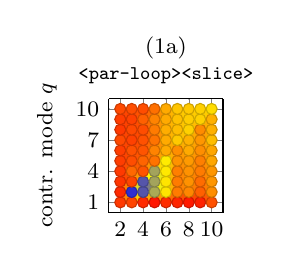
\begin{tikzpicture}
\begin{axis}
[%
width=0.25\textwidth,
height=0.25\textwidth,
style={font=\footnotesize},
grid=major,
grid style={dotted},
align=center,
ylabel={contr. mode $q$},
title={(1a)\\\tss{<par-loop><slice>}}, %  ompfor<slice>, asymmetric, row-major
title style={yshift=-1ex},
scaled ticks=false,
zlabel={GFlops/core},
view={0}{90},
ytick={1,4,7,10},
xtick={2,4,6,8,10},
xmin=1, xmax=11,
ymin=0, ymax=11,
try min ticks=8,
zmin=0, 
zmax=55,
point meta min=0,
point meta max=55,
colormap/hot%
]
\addplot3[contour filled={number=100},scatter,shader=flat]%
coordinates{%
(2.000,1.000,46.205) (2.000,2.000,48.432) (2.000,3.000,46.757) (2.000,4.000,46.289) (2.000,5.000,45.849) (2.000,6.000,45.967) (2.000,7.000,44.204) (2.000,8.000,46.356) (2.000,9.000,45.926) (2.000,10.000,44.107)

(3.000,1.000,44.709) (3.000,2.000,3.490) (3.000,3.000,45.092) (3.000,4.000,39.661) (3.000,5.000,43.650) (3.000,6.000,42.987) (3.000,7.000,45.255) (3.000,8.000,44.199) (3.000,9.000,45.386) (3.000,10.000,43.884)

(4.000,1.000,48.439) (4.000,2.000,6.592) (4.000,3.000,6.547) (4.000,4.000,42.608) (4.000,5.000,40.353) (4.000,6.000,42.793) (4.000,7.000,43.427) (4.000,8.000,43.502) (4.000,9.000,41.022) (4.000,10.000,43.468)

(5.000,1.000,51.698) (5.000,2.000,12.102) (5.000,3.000,11.990) (5.000,4.000,11.787) (5.000,5.000,38.340) (5.000,6.000,35.786) (5.000,7.000,38.337) (5.000,8.000,36.881) (5.000,9.000,35.985) (5.000,10.000,38.867)

(6.000,1.000,48.224) (6.000,2.000,22.132) (6.000,3.000,22.154) (6.000,4.000,21.599) (6.000,5.000,20.923) (6.000,6.000,30.377) (6.000,7.000,30.679) (6.000,8.000,30.242) (6.000,9.000,30.268) (6.000,10.000,30.774)

(7.000,1.000,49.015) (7.000,2.000,37.193) (7.000,3.000,37.287) (7.000,4.000,36.560) (7.000,5.000,34.085) (7.000,6.000,34.150) (7.000,7.000,26.230) (7.000,8.000,27.547) (7.000,9.000,27.309) (7.000,10.000,26.404)

(8.000,1.000,50.951) (8.000,2.000,35.202) (8.000,3.000,33.857) (8.000,4.000,33.637) (8.000,5.000,32.857) (8.000,6.000,30.480) (8.000,7.000,29.367) (8.000,8.000,25.217) (8.000,9.000,25.569) (8.000,10.000,25.965)

(9.000,1.000,49.499) (9.000,2.000,40.851) (9.000,3.000,39.445) (9.000,4.000,37.174) (9.000,5.000,36.460) (9.000,6.000,34.357) (9.000,7.000,33.387) (9.000,8.000,35.082) (9.000,9.000,25.196) (9.000,10.000,24.841)

(10.000,1.000,43.332) (10.000,2.000,34.399) (10.000,3.000,33.017) (10.000,4.000,33.056) (10.000,5.000,31.245) (10.000,6.000,30.900) (10.000,7.000,27.520) (10.000,8.000,29.561) (10.000,9.000,29.464) (10.000,10.000,23.270)
};
\end{axis}
\end{tikzpicture}
\hfill
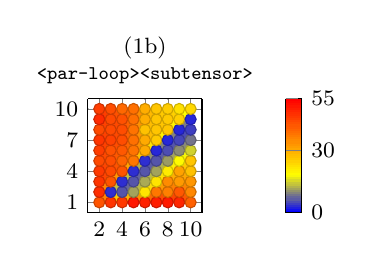
\begin{tikzpicture}
\begin{axis}
[%
width=0.25\textwidth,
height=0.25\textwidth,
style={font=\footnotesize},
grid=major,
grid style={dotted},
align=center,
title={(1b)\\\tss{<par-loop><subtensor>}}, %  ompfor<subtensor>, asymmetric, mkl, row.major
title style={yshift=-1ex},
scaled ticks=false,
zlabel={GFlops},
view={0}{90}, 
ytick={1,4,7,10},
xtick={2,4,6,8,10},
xmin=1,
xmax=11,
ymin=0,
ymax=11,
try min ticks=8,
zmin=0,
zmax=55,
point meta min=0,
point meta max=55,
colormap/hot, 
colorbar sampled,
colorbar/width=0.2cm,
colorbar style={
point meta min=0, 
point meta max=55,
samples=55,
font=\footnotesize,
ytick={0,30,55},
yticklabels={0,30,55}
}
]
\addplot3[contour filled={number=100},scatter,shader=flat]%
coordinates{%
(2.000,1.000,42.701) (2.000,2.000,48.025) (2.000,3.000,46.960) (2.000,4.000,46.462) (2.000,5.000,44.445) (2.000,6.000,45.870) (2.000,7.000,47.088) (2.000,8.000,44.348) (2.000,9.000,48.456) (2.000,10.000,46.026)

(3.000,1.000,46.781) (3.000,2.000,3.490) (3.000,3.000,42.650) (3.000,4.000,44.094) (3.000,5.000,43.649) (3.000,6.000,43.013) (3.000,7.000,45.421) (3.000,8.000,44.471) (3.000,9.000,44.445) (3.000,10.000,43.995)

(4.000,1.000,46.527) (4.000,2.000,6.577) (4.000,3.000,3.499) (4.000,4.000,42.546) (4.000,5.000,40.416) (4.000,6.000,41.868) (4.000,7.000,43.819) (4.000,8.000,43.998) (4.000,9.000,43.351) (4.000,10.000,40.021)

(5.000,1.000,51.554) (5.000,2.000,12.076) (5.000,3.000,6.515) (5.000,4.000,3.499) (5.000,5.000,37.797) (5.000,6.000,38.071) (5.000,7.000,38.883) (5.000,8.000,38.063) (5.000,9.000,38.851) (5.000,10.000,38.658)

(6.000,1.000,49.690) (6.000,2.000,22.187) (6.000,3.000,12.144) (6.000,4.000,6.539) (6.000,5.000,3.424) (6.000,6.000,30.342) (6.000,7.000,30.321) (6.000,8.000,27.451) (6.000,9.000,29.990) (6.000,10.000,29.820)

(7.000,1.000,50.276) (7.000,2.000,37.556) (7.000,3.000,22.201) (7.000,4.000,12.061) (7.000,5.000,6.180) (7.000,6.000,3.242) (7.000,7.000,25.893) (7.000,8.000,26.624) (7.000,9.000,26.558) (7.000,10.000,26.433)

(8.000,1.000,50.756) (8.000,2.000,36.461) (8.000,3.000,34.923) (8.000,4.000,21.265) (8.000,5.000,11.303) (8.000,6.000,5.845) (8.000,7.000,3.198) (8.000,8.000,26.517) (8.000,9.000,26.008) (8.000,10.000,25.785)

(9.000,1.000,49.420) (9.000,2.000,41.812) (9.000,3.000,32.592) (9.000,4.000,31.403) (9.000,5.000,19.209) (9.000,6.000,10.301) (9.000,7.000,5.455) (9.000,8.000,3.150) (9.000,9.000,24.977) (9.000,10.000,22.639)

(10.000,1.000,41.095) (10.000,2.000,35.514) (10.000,3.000,33.514) (10.000,4.000,27.410) (10.000,5.000,26.443) (10.000,6.000,15.285) (10.000,7.000,8.666) (10.000,8.000,4.913) (10.000,9.000,2.865) (10.000,10.000,23.899)
};
\end{axis}
\end{tikzpicture}
\hfill
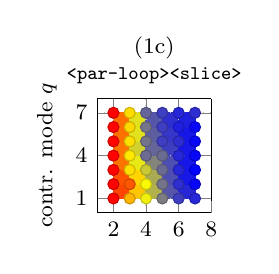
\begin{tikzpicture}
\begin{axis}
[
width=0.25\textwidth,
height=0.25\textwidth,
style={font=\footnotesize},
grid=major,
grid style={dotted},
align=center,
%xlabel={tensor order},
ylabel={contr. mode $q$},
title={(1c)\\\tss{<par-loop><slice>}}, %  ompfor<slice>, symmetric, row-major
title style={yshift=-1ex},
scaled ticks=false,
zlabel={GFlops},
view={0}{90}, 
ytick={1,4,7,10},
xtick={2,4,6,8},
xmin=1, xmax=8,
ymin=0, ymax=8,
try min ticks=8,
zmin=0, zmax=55,
point meta min=0, point meta max=55,
colormap/hot
]
\addplot3[contour filled={number=100},scatter,shader=flat]
coordinates{%
(2.000,1.000,54.129) (2.000,2.000,54.324) (2.000,3.000,53.906) (2.000,4.000,54.242) (2.000,5.000,53.858) (2.000,6.000,54.180) (2.000,7.000,54.829)

(3.000,1.000,28.630) (3.000,2.000,42.238) (3.000,3.000,22.607) (3.000,4.000,21.517) (3.000,5.000,22.772) (3.000,6.000,23.844) (3.000,7.000,23.517)

(4.000,1.000,17.109) (4.000,2.000,17.647) (4.000,3.000,14.726) (4.000,4.000,8.173) (4.000,5.000,8.610) (4.000,6.000,8.769) (4.000,7.000,7.699)

(5.000,1.000,8.862) (5.000,2.000,8.565) (5.000,3.000,8.163) (5.000,4.000,8.073) (5.000,5.000,4.852) (5.000,6.000,4.491) (5.000,7.000,4.928)

(6.000,1.000,4.508) (6.000,2.000,3.408) (6.000,3.000,3.251) (6.000,4.000,3.232) (6.000,5.000,3.476) (6.000,6.000,2.736) (6.000,7.000,2.893)

(7.000,1.000,3.212) (7.000,2.000,0.631) (7.000,3.000,0.521) (7.000,4.000,0.567) (7.000,5.000,0.661) (7.000,6.000,0.594) (7.000,7.000,3.421)
};
\end{axis}
\end{tikzpicture}
\hfill
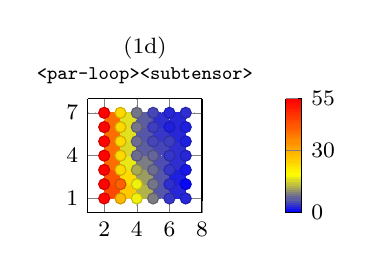
\begin{tikzpicture}
\begin{axis}
[%
width=0.25\textwidth,
height=0.25\textwidth,
style={font=\footnotesize},
grid=major,
grid style={dotted},
align=center,
title={(1d)\\\tss{<par-loop><subtensor>}},%  ompfor<subtensor>, symmetric, row-major
title style={yshift=-1ex},
scaled ticks=false,
zlabel={GFlops},
view={0}{90}, 
ytick={1,4,7,10},
xtick={2,4,6,8},
xmin=1, xmax=8,
ymin=0, ymax=8,
try min ticks=8,
zmin=0, zmax=55,
point meta min=0, 
point meta max=55,
colormap/hot,
colorbar sampled,
colorbar/width=0.2cm,
colorbar style={
point meta min=0, 
point meta max=55,
samples=55,
font=\footnotesize,
ytick={0,30,55},
yticklabels={0,30,55}
}
]
\addplot3[contour filled={number=100}, scatter, shader=flat]
coordinates{
(2.000,1.000,53.767) (2.000,2.000,54.181) (2.000,3.000,54.001) (2.000,4.000,54.390) (2.000,5.000,54.441) (2.000,6.000,54.194) (2.000,7.000,54.903)

(3.000,1.000,28.554) (3.000,2.000,40.760) (3.000,3.000,23.879) (3.000,4.000,24.014) (3.000,5.000,23.825) (3.000,6.000,23.858) (3.000,7.000,23.926)

(4.000,1.000,17.238) (4.000,2.000,17.309) (4.000,3.000,12.158) (4.000,4.000,7.940) (4.000,5.000,7.894) (4.000,6.000,8.693) (4.000,7.000,8.692)

(5.000,1.000,9.003) (5.000,2.000,8.513) (5.000,3.000,8.209) (5.000,4.000,7.470) (5.000,5.000,5.029) (5.000,6.000,4.696) (5.000,7.000,5.111)

(6.000,1.000,4.345) (6.000,2.000,3.345) (6.000,3.000,4.194) (6.000,4.000,4.024) (6.000,5.000,4.933) (6.000,6.000,2.694) (6.000,7.000,2.830)

(7.000,1.000,2.768) (7.000,2.000,0.619) (7.000,3.000,2.198) (7.000,4.000,3.270) (7.000,5.000,2.670) (7.000,6.000,2.495) (7.000,7.000,3.356)
};
\end{axis}
\end{tikzpicture}

\input{fig.performance.tlib.contour-mkl-pargemm} 
\caption{%
\footnotesize %
Performance contour plots in double-precision GFLOPS/core of the proposed TTM algorithms \tf{<par-loop>} and \tf{<par-gemm>} with varying tensor orders $p$ and contraction modes $q$. 
The top row of maps (1x) depict measurements of the \tf{<par-loop>} versions while the bottom row of maps with number (2x) contain measurements of the \tf{<par-gemm>} versions.
Tensors are asymmetrically shaped on the left four maps (a,b) and symmetrically shaped on the right four maps (c,d).
Tensor $\mubA$ and $\mubC$ have the first-order while matrix $\mbB$ has the row-major ordering.
All functions have been measured on an Intel Xeon Gold 5318Y.
\label{fig:performance.tlib.contour}
}
\end{figure*}


\begin{figure*}[t]
\input{fig.performance.tlib.case8-cdf-mkl}
\input{fig.performance.tlib.case8-cdf-aocl}
\caption{ %
\footnotesize%
Cumulative performance distributions in double-precision GFLOPS/core of the proposed algorithms for the eighth case.
Each distribution belongs to one algorithm:
\tf{<batched-gemm>} (\ref{coord:gemm_batch}), %
\tf{<combined>} (\ref{coord:optimized}),
\tf{<par-gemm>,slice>} (\ref{coord:seq_loops_par_gemm_slice}) and
\tf{<par-loop,slice>} (\ref{coord:par_loops_seq_gemm_slice}),
\tf{<par-gemm,subtensor>} (\ref{coord:seq_loops_par_gemm_subtensor}) and
\tf{<par-loop,subtensor>} (\ref{coord:par_loops_seq_gemm_subtensor}).
The top row of maps (1x) depict measurements performed on an Intel Xeon Gold 5318Y with the MKL while the bottom row of maps with number (2x) contain measurements performed on an AMD EPYC 9354 with the AOCL.
Tensors are asymmetrically shaped in (a) and (b) and symmetrically shaped in (c) and (d).
Input matrix has the row-major ordering (rm) in (a) and (c) and column-major ordering (cm) in (b) and (d).
}
\label{fig:performance.tlib.case8}
\end{figure*}


\begin{figure*}[t]
\input{fig.performance.tlib.format.mkl}
\input{fig.performance.tlib.format.aocl}
%\input{fig.performance.tlib.format}
\caption{ %
\footnotesize%
Box plots visualizing performance statics in double-precision GFLOPS/core of the function with row-major (left) or column-major matrices (right).
Box plot number $k$ denotes the $k$-order tensor layout of symmetrically shaped tensors with order $7$.
% where the $1$-order and $7$-order layouts are the first- and last-order storage formats, respectively.
}
\label{fig:performance.tlib.format}
\end{figure*}

\begin{figure*}[t]
\centering
\tikzset{every mark/.append style={scale=1.5}}
\begin{tikzpicture}
\begin{axis}[
height=0.3\textheight,
width=0.45\textwidth,
style={font=\footnotesize},
grid=major,
grid style={dotted},
align=center,
ylabel={GFLOPS/core},
%xlabel={Test Cases [\%]},
xlabel near ticks,
title={Intel Xeon Gold 5318Y (nonsymmetric)},
title style={yshift=-1.5ex},
ytick={0,10,20,30,40,50,60},
yticklabels={0,10,20,30,40,50,60},
xtick={0,0.25,0.5,0.75,1},
xticklabels={0,25,50,75,100},
mark repeat={16},
ymax=60,
cycle list name=compare other libraries for mkl
]
\addplot%%+[const plo, line width=1,mark options={scale=2}]
coordinates{(0.000,9.389) (0.001,9.389) (0.003,10.664) (0.004,10.927) (0.006,11.198) (0.007,11.503) (0.008,11.776) (0.010,12.442) (0.011,12.740) (0.013,13.399) (0.014,13.509) (0.015,15.991) (0.017,17.359) (0.018,17.578) (0.019,18.131) (0.021,18.461) (0.022,18.862) (0.024,19.710) (0.025,19.763) (0.026,19.785) (0.028,19.888) (0.029,20.125) (0.031,20.201) (0.032,20.312) (0.033,20.754) (0.035,20.802) (0.036,20.883) (0.038,21.000) (0.039,21.016) (0.040,21.023) (0.042,21.042) (0.043,21.218) (0.044,21.244) (0.046,21.276) (0.047,21.409) (0.049,21.411) (0.050,21.510) (0.051,21.524) (0.053,21.533) (0.054,21.850) (0.056,21.872) (0.057,22.083) (0.058,22.112) (0.060,22.165) (0.061,22.165) (0.062,22.242) (0.064,22.247) (0.065,22.848) (0.067,23.011) (0.068,23.129) (0.069,23.194) (0.071,23.409) (0.072,23.478) (0.074,23.634) (0.075,23.671) (0.076,24.058) (0.078,24.102) (0.079,24.181) (0.081,24.231) (0.082,24.385) (0.083,24.457) (0.085,24.632) (0.086,24.768) (0.087,24.822) (0.089,24.872) (0.090,25.059) (0.092,25.114) (0.093,25.141) (0.094,25.211) (0.096,25.274) (0.097,25.304) (0.099,25.337) (0.100,25.360) (0.101,25.447) (0.103,25.480) (0.104,25.497) (0.106,25.529) (0.107,25.546) (0.108,25.583) (0.110,25.627) (0.111,25.630) (0.113,25.687) (0.114,25.701) (0.115,25.728) (0.117,25.729) (0.118,25.737) (0.119,25.841) (0.121,25.862) (0.122,25.955) (0.124,26.071) (0.125,26.154) (0.126,26.173) (0.128,26.192) (0.129,26.233) (0.131,26.252) (0.132,26.273) (0.133,26.341) (0.135,26.344) (0.136,26.359) (0.138,26.409) (0.139,26.427) (0.140,26.440) (0.142,26.537) (0.143,26.606) (0.144,26.607) (0.146,26.618) (0.147,26.690) (0.149,26.719) (0.150,27.033) (0.151,27.043) (0.153,27.333) (0.154,27.337) (0.156,27.530) (0.157,27.618) (0.158,27.629) (0.160,27.703) (0.161,27.800) (0.163,27.893) (0.164,27.933) (0.165,27.977) (0.167,27.998) (0.168,28.076) (0.169,28.100) (0.171,28.185) (0.172,28.268) (0.174,28.326) (0.175,28.397) (0.176,28.418) (0.178,28.451) (0.179,28.454) (0.181,28.490) (0.182,28.610) (0.183,28.682) (0.185,28.726) (0.186,28.790) (0.188,28.810) (0.189,28.847) (0.190,28.861) (0.192,28.935) (0.193,28.975) (0.194,29.007) (0.196,29.039) (0.197,29.136) (0.199,29.150) (0.200,29.217) (0.201,29.309) (0.203,29.331) (0.204,29.337) (0.206,29.459) (0.207,29.537) (0.208,29.645) (0.210,29.649) (0.211,29.654) (0.212,29.672) (0.214,29.698) (0.215,29.784) (0.217,29.846) (0.218,29.882) (0.219,29.897) (0.221,29.900) (0.222,29.905) (0.224,29.905) (0.225,29.911) (0.226,30.031) (0.228,30.034) (0.229,30.145) (0.231,30.146) (0.232,30.169) (0.233,30.174) (0.235,30.225) (0.236,30.294) (0.238,30.367) (0.239,30.371) (0.240,30.453) (0.242,30.505) (0.243,30.512) (0.244,30.527) (0.246,30.531) (0.247,30.546) (0.249,30.579) (0.250,30.600) (0.251,30.647) (0.253,30.665) (0.254,30.685) (0.256,30.699) (0.257,30.752) (0.258,30.760) (0.260,30.794) (0.261,30.942) (0.263,30.964) (0.264,30.990) (0.265,30.992) (0.267,31.062) (0.268,31.070) (0.269,31.087) (0.271,31.129) (0.272,31.172) (0.274,31.304) (0.275,31.320) (0.276,31.341) (0.278,31.348) (0.279,31.478) (0.281,31.589) (0.282,31.627) (0.283,31.714) (0.285,31.930) (0.286,32.000) (0.288,32.004) (0.289,32.121) (0.290,32.174) (0.292,32.238) (0.293,32.303) (0.294,32.325) (0.296,32.366) (0.297,32.415) (0.299,32.663) (0.300,32.752) (0.301,32.847) (0.303,32.851) (0.304,32.886) (0.306,33.031) (0.307,33.040) (0.308,33.042) (0.310,33.127) (0.311,33.424) (0.312,33.546) (0.314,33.567) (0.315,33.573) (0.317,33.578) (0.318,33.597) (0.319,33.646) (0.321,33.683) (0.322,33.718) (0.324,33.767) (0.325,33.770) (0.326,33.787) (0.328,33.854) (0.329,33.938) (0.331,33.962) (0.332,34.102) (0.333,34.142) (0.335,34.247) (0.336,34.310) (0.338,34.311) (0.339,34.336) (0.340,34.366) (0.342,34.396) (0.343,34.405) (0.344,34.570) (0.346,34.646) (0.347,34.662) (0.349,34.712) (0.350,34.821) (0.351,34.980) (0.353,35.008) (0.354,35.010) (0.356,35.051) (0.357,35.088) (0.358,35.111) (0.360,35.129) (0.361,35.252) (0.362,35.269) (0.364,35.313) (0.365,35.372) (0.367,35.388) (0.368,35.419) (0.369,35.425) (0.371,35.473) (0.372,35.480) (0.374,35.523) (0.375,35.534) (0.376,35.611) (0.378,35.647) (0.379,35.649) (0.381,35.669) (0.382,35.687) (0.383,35.832) (0.385,35.847) (0.386,35.914) (0.388,35.931) (0.389,35.943) (0.390,35.971) (0.392,35.988) (0.393,36.010) (0.394,36.019) (0.396,36.130) (0.397,36.246) (0.399,36.301) (0.400,36.325) (0.401,36.332) (0.403,36.346) (0.404,36.357) (0.406,36.379) (0.407,36.412) (0.408,36.415) (0.410,36.481) (0.411,36.485) (0.413,36.485) (0.414,36.524) (0.415,36.532) (0.417,36.560) (0.418,36.569) (0.419,36.631) (0.421,36.685) (0.422,36.687) (0.424,36.782) (0.425,36.842) (0.426,36.853) (0.428,36.855) (0.429,36.898) (0.431,36.908) (0.432,36.910) (0.433,36.928) (0.435,36.930) (0.436,36.942) (0.438,36.953) (0.439,36.964) (0.440,36.974) (0.442,36.993) (0.443,37.008) (0.444,37.062) (0.446,37.063) (0.447,37.127) (0.449,37.140) (0.450,37.146) (0.451,37.148) (0.453,37.149) (0.454,37.197) (0.456,37.240) (0.457,37.262) (0.458,37.272) (0.460,37.302) (0.461,37.319) (0.463,37.347) (0.464,37.357) (0.465,37.361) (0.467,37.537) (0.468,37.538) (0.469,37.594) (0.471,37.629) (0.472,37.685) (0.474,37.704) (0.475,37.714) (0.476,37.740) (0.478,37.768) (0.479,37.770) (0.481,37.802) (0.482,37.837) (0.483,37.863) (0.485,37.877) (0.486,37.962) (0.487,37.976) (0.489,37.991) (0.490,38.002) (0.492,38.015) (0.493,38.037) (0.494,38.044) (0.496,38.122) (0.497,38.127) (0.499,38.141) (0.500,38.203) (0.501,38.233) (0.503,38.257) (0.504,38.279) (0.506,38.301) (0.507,38.350) (0.508,38.375) (0.510,38.419) (0.511,38.420) (0.512,38.439) (0.514,38.470) (0.515,38.475) (0.517,38.519) (0.518,38.537) (0.519,38.550) (0.521,38.567) (0.522,38.578) (0.524,38.598) (0.525,38.605) (0.526,38.620) (0.528,38.628) (0.529,38.824) (0.531,38.857) (0.532,38.953) (0.533,39.159) (0.535,39.289) (0.536,39.299) (0.537,39.479) (0.539,39.502) (0.540,39.516) (0.542,39.519) (0.543,39.540) (0.544,39.588) (0.546,39.594) (0.547,39.643) (0.549,39.744) (0.550,39.806) (0.551,39.807) (0.553,39.879) (0.554,39.948) (0.556,40.039) (0.557,40.105) (0.558,40.122) (0.560,40.192) (0.561,40.327) (0.562,40.346) (0.564,40.353) (0.565,40.418) (0.567,40.424) (0.568,40.516) (0.569,40.539) (0.571,40.553) (0.572,40.579) (0.574,40.581) (0.575,40.585) (0.576,40.590) (0.578,40.602) (0.579,40.666) (0.581,40.685) (0.582,40.700) (0.583,40.710) (0.585,40.811) (0.586,40.880) (0.587,40.909) (0.589,40.946) (0.590,40.951) (0.592,40.956) (0.593,40.962) (0.594,40.970) (0.596,41.019) (0.597,41.032) (0.599,41.040) (0.600,41.076) (0.601,41.077) (0.603,41.110) (0.604,41.127) (0.606,41.132) (0.607,41.133) (0.608,41.137) (0.610,41.138) (0.611,41.152) (0.613,41.161) (0.614,41.183) (0.615,41.224) (0.617,41.242) (0.618,41.259) (0.619,41.295) (0.621,41.333) (0.622,41.360) (0.624,41.370) (0.625,41.376) (0.626,41.389) (0.628,41.432) (0.629,41.439) (0.631,41.460) (0.632,41.579) (0.633,41.654) (0.635,41.658) (0.636,41.659) (0.637,41.663) (0.639,41.687) (0.640,41.773) (0.642,41.805) (0.643,41.832) (0.644,41.834) (0.646,41.846) (0.647,41.847) (0.649,41.875) (0.650,41.881) (0.651,41.882) (0.653,41.972) (0.654,42.045) (0.656,42.088) (0.657,42.156) (0.658,42.173) (0.660,42.185) (0.661,42.212) (0.662,42.231) (0.664,42.274) (0.665,42.279) (0.667,42.305) (0.668,42.308) (0.669,42.368) (0.671,42.389) (0.672,42.412) (0.674,42.451) (0.675,42.458) (0.676,42.462) (0.678,42.486) (0.679,42.544) (0.681,42.553) (0.682,42.588) (0.683,42.601) (0.685,42.607) (0.686,42.626) (0.688,42.679) (0.689,42.725) (0.690,42.726) (0.692,42.819) (0.693,42.844) (0.694,42.845) (0.696,42.866) (0.697,42.886) (0.699,42.917) (0.700,42.918) (0.701,42.985) (0.703,43.030) (0.704,43.071) (0.706,43.182) (0.707,43.182) (0.708,43.191) (0.710,43.305) (0.711,43.315) (0.712,43.375) (0.714,43.402) (0.715,43.414) (0.717,43.425) (0.718,43.443) (0.719,43.465) (0.721,43.476) (0.722,43.483) (0.724,43.503) (0.725,43.535) (0.726,43.557) (0.728,43.631) (0.729,43.686) (0.731,43.728) (0.732,43.733) (0.733,43.780) (0.735,43.790) (0.736,43.808) (0.738,43.836) (0.739,43.844) (0.740,43.863) (0.742,43.870) (0.743,43.945) (0.744,43.966) (0.746,44.014) (0.747,44.024) (0.749,44.031) (0.750,44.080) (0.751,44.116) (0.753,44.118) (0.754,44.156) (0.756,44.179) (0.757,44.200) (0.758,44.241) (0.760,44.285) (0.761,44.307) (0.762,44.320) (0.764,44.322) (0.765,44.327) (0.767,44.339) (0.768,44.397) (0.769,44.427) (0.771,44.427) (0.772,44.456) (0.774,44.505) (0.775,44.532) (0.776,44.600) (0.778,44.640) (0.779,44.643) (0.781,44.647) (0.782,44.680) (0.783,44.727) (0.785,44.763) (0.786,44.793) (0.787,44.822) (0.789,44.834) (0.790,44.850) (0.792,44.873) (0.793,44.891) (0.794,44.897) (0.796,44.917) (0.797,44.929) (0.799,44.935) (0.800,45.082) (0.801,45.092) (0.803,45.126) (0.804,45.182) (0.806,45.189) (0.807,45.200) (0.808,45.213) (0.810,45.220) (0.811,45.227) (0.812,45.337) (0.814,45.371) (0.815,45.372) (0.817,45.418) (0.818,45.441) (0.819,45.481) (0.821,45.498) (0.822,45.544) (0.824,45.589) (0.825,45.610) (0.826,45.610) (0.828,45.617) (0.829,45.662) (0.831,45.662) (0.832,45.668) (0.833,45.692) (0.835,45.738) (0.836,45.743) (0.838,45.774) (0.839,45.806) (0.840,45.844) (0.842,45.845) (0.843,45.864) (0.844,45.895) (0.846,45.912) (0.847,45.915) (0.849,45.927) (0.850,45.942) (0.851,45.988) (0.853,46.029) (0.854,46.045) (0.856,46.061) (0.857,46.085) (0.858,46.120) (0.860,46.131) (0.861,46.324) (0.863,46.357) (0.864,46.422) (0.865,46.470) (0.867,46.521) (0.868,46.531) (0.869,46.554) (0.871,46.586) (0.872,46.635) (0.874,46.638) (0.875,46.647) (0.876,46.664) (0.878,46.681) (0.879,46.787) (0.881,46.810) (0.882,46.836) (0.883,46.856) (0.885,46.871) (0.886,46.958) (0.887,46.995) (0.889,47.002) (0.890,47.045) (0.892,47.053) (0.893,47.113) (0.894,47.226) (0.896,47.314) (0.897,47.501) (0.899,47.524) (0.900,47.541) (0.901,47.618) (0.903,47.636) (0.904,47.666) (0.906,47.683) (0.907,47.730) (0.908,47.752) (0.910,47.773) (0.911,47.774) (0.912,47.809) (0.914,47.816) (0.915,47.928) (0.917,47.953) (0.918,48.058) (0.919,48.070) (0.921,48.106) (0.922,48.174) (0.924,48.203) (0.925,48.407) (0.926,48.421) (0.928,48.423) (0.929,48.570) (0.931,48.666) (0.932,48.676) (0.933,48.708) (0.935,48.805) (0.936,49.029) (0.938,49.113) (0.939,49.402) (0.940,49.463) (0.942,49.502) (0.943,49.570) (0.944,49.627) (0.946,49.636) (0.947,49.731) (0.949,49.758) (0.950,49.774) (0.951,49.812) (0.953,49.864) (0.954,49.903) (0.956,49.981) (0.957,50.099) (0.958,50.331) (0.960,50.422) (0.961,50.482) (0.963,50.652) (0.964,50.668) (0.965,50.672) (0.967,50.757) (0.968,50.770) (0.969,50.839) (0.971,50.888) (0.972,50.946) (0.974,50.979) (0.975,51.209) (0.976,51.254) (0.978,51.612) (0.979,51.646) (0.981,51.654) (0.982,52.127) (0.983,52.295) (0.985,52.836) (0.986,52.897) (0.988,52.915) (0.989,53.597) (0.990,53.597) (0.992,53.621) (0.993,53.886) (0.994,53.955) (0.996,55.820) (0.997,57.147) (0.999,57.169) (1.000,57.820) };
\label{coord:nonsymmetric.tlib.slice}

\addplot
coordinates{(0.000,7.134) (0.002,7.137) (0.003,7.175) (0.005,7.225) (0.006,7.349) (0.008,7.671) (0.009,7.733) (0.011,7.925) (0.012,11.469) (0.014,11.827) (0.015,12.079) (0.017,12.245) (0.019,12.336) (0.020,12.497) (0.022,12.584) (0.023,12.781) (0.025,12.932) (0.026,12.952) (0.028,12.980) (0.029,13.203) (0.031,13.246) (0.032,13.339) (0.034,13.847) (0.036,15.815) (0.037,15.855) (0.039,16.093) (0.040,16.338) (0.042,16.361) (0.043,16.439) (0.045,16.479) (0.046,16.645) (0.048,16.662) (0.049,16.675) (0.051,16.846) (0.053,17.321) (0.054,17.518) (0.056,17.608) (0.057,17.654) (0.059,17.656) (0.060,17.835) (0.062,18.025) (0.063,18.106) (0.065,18.312) (0.066,18.353) (0.068,18.411) (0.070,18.536) (0.071,18.780) (0.073,18.788) (0.074,18.791) (0.076,18.861) (0.077,18.967) (0.079,19.079) (0.080,19.131) (0.082,19.144) (0.083,19.165) (0.085,19.177) (0.087,19.189) (0.088,19.434) (0.090,19.681) (0.091,19.863) (0.093,19.958) (0.094,19.981) (0.096,19.985) (0.097,20.037) (0.099,20.069) (0.100,20.325) (0.102,20.447) (0.104,20.642) (0.105,20.670) (0.107,20.730) (0.108,20.828) (0.110,20.917) (0.111,20.964) (0.113,20.993) (0.114,20.999) (0.116,21.021) (0.117,21.100) (0.119,21.111) (0.121,21.233) (0.122,21.255) (0.124,21.262) (0.125,21.328) (0.127,21.439) (0.128,21.451) (0.130,21.521) (0.131,21.602) (0.133,21.624) (0.134,21.626) (0.136,21.629) (0.138,21.640) (0.139,21.656) (0.141,21.656) (0.142,21.671) (0.144,21.726) (0.145,21.739) (0.147,21.742) (0.148,21.877) (0.150,21.880) (0.151,21.884) (0.153,21.942) (0.155,21.960) (0.156,21.972) (0.158,21.981) (0.159,22.100) (0.161,22.147) (0.162,22.154) (0.164,22.171) (0.165,22.221) (0.167,22.271) (0.168,22.312) (0.170,22.366) (0.172,22.373) (0.173,22.383) (0.175,22.442) (0.176,22.501) (0.178,22.504) (0.179,22.552) (0.181,22.567) (0.182,22.578) (0.184,22.580) (0.185,22.601) (0.187,22.615) (0.189,22.616) (0.190,22.681) (0.192,22.687) (0.193,22.693) (0.195,22.708) (0.196,22.715) (0.198,22.819) (0.199,22.829) (0.201,22.835) (0.202,22.842) (0.204,22.843) (0.206,22.846) (0.207,22.873) (0.209,22.884) (0.210,22.959) (0.212,22.988) (0.213,22.994) (0.215,23.036) (0.216,23.162) (0.218,23.172) (0.219,23.273) (0.221,23.288) (0.223,23.482) (0.224,23.502) (0.226,23.529) (0.227,23.550) (0.229,23.645) (0.230,23.649) (0.232,23.673) (0.233,23.689) (0.235,23.731) (0.236,23.733) (0.238,23.742) (0.240,23.762) (0.241,23.762) (0.243,23.771) (0.244,23.773) (0.246,23.897) (0.247,23.948) (0.249,23.963) (0.250,23.981) (0.252,24.001) (0.253,24.009) (0.255,24.046) (0.257,24.073) (0.258,24.099) (0.260,24.127) (0.261,24.147) (0.263,24.168) (0.264,24.170) (0.266,24.184) (0.267,24.187) (0.269,24.202) (0.270,24.211) (0.272,24.224) (0.274,24.258) (0.275,24.282) (0.277,24.344) (0.278,24.356) (0.280,24.387) (0.281,24.410) (0.283,24.461) (0.284,24.513) (0.286,24.551) (0.287,24.568) (0.289,24.577) (0.291,24.593) (0.292,24.635) (0.294,24.646) (0.295,24.646) (0.297,24.669) (0.298,24.671) (0.300,24.688) (0.301,24.705) (0.303,24.798) (0.304,24.804) (0.306,24.816) (0.308,24.852) (0.309,24.941) (0.311,25.008) (0.312,25.033) (0.314,25.036) (0.315,25.129) (0.317,25.161) (0.318,25.162) (0.320,25.238) (0.321,25.257) (0.323,25.290) (0.325,25.365) (0.326,25.478) (0.328,25.518) (0.329,25.545) (0.331,25.587) (0.332,25.609) (0.334,25.625) (0.335,25.627) (0.337,25.699) (0.338,25.734) (0.340,25.762) (0.342,25.762) (0.343,25.788) (0.345,25.797) (0.346,25.800) (0.348,25.819) (0.349,25.828) (0.351,25.834) (0.352,25.835) (0.354,25.892) (0.355,25.905) (0.357,25.927) (0.359,25.945) (0.360,25.946) (0.362,25.984) (0.363,26.095) (0.365,26.108) (0.366,26.167) (0.368,26.211) (0.369,26.233) (0.371,26.237) (0.372,26.238) (0.374,26.279) (0.376,26.354) (0.377,26.367) (0.379,26.369) (0.380,26.387) (0.382,26.387) (0.383,26.400) (0.385,26.482) (0.386,26.491) (0.388,26.549) (0.389,26.583) (0.391,26.603) (0.393,26.622) (0.394,26.650) (0.396,26.671) (0.397,26.708) (0.399,26.848) (0.400,26.909) (0.402,26.935) (0.403,26.956) (0.405,26.964) (0.406,27.050) (0.408,27.181) (0.410,27.208) (0.411,27.212) (0.413,27.212) (0.414,27.285) (0.416,27.413) (0.417,27.455) (0.419,28.206) (0.420,28.478) (0.422,28.498) (0.423,28.681) (0.425,28.846) (0.427,28.926) (0.428,28.931) (0.430,29.288) (0.431,29.309) (0.433,29.345) (0.434,29.348) (0.436,29.456) (0.437,29.553) (0.439,29.586) (0.440,29.605) (0.442,29.641) (0.444,29.668) (0.445,29.672) (0.447,29.680) (0.448,29.691) (0.450,29.692) (0.451,29.740) (0.453,29.740) (0.454,29.754) (0.456,29.810) (0.457,29.849) (0.459,29.852) (0.461,29.857) (0.462,29.857) (0.464,29.882) (0.465,29.906) (0.467,29.919) (0.468,29.931) (0.470,29.931) (0.471,29.942) (0.473,29.945) (0.474,29.954) (0.476,29.965) (0.478,29.994) (0.479,30.001) (0.481,30.045) (0.482,30.051) (0.484,30.069) (0.485,30.085) (0.487,30.176) (0.488,30.177) (0.490,30.178) (0.491,30.191) (0.493,30.291) (0.495,30.357) (0.496,30.391) (0.498,30.392) (0.499,30.439) (0.501,30.481) (0.502,30.521) (0.504,30.639) (0.505,30.679) (0.507,30.691) (0.509,30.713) (0.510,30.725) (0.512,30.742) (0.513,30.820) (0.515,30.874) (0.516,30.909) (0.518,30.928) (0.519,31.100) (0.521,31.404) (0.522,31.522) (0.524,31.626) (0.526,31.683) (0.527,32.351) (0.529,32.504) (0.530,32.635) (0.532,32.726) (0.533,32.832) (0.535,33.106) (0.536,33.246) (0.538,33.471) (0.539,33.852) (0.541,34.010) (0.543,34.107) (0.544,34.109) (0.546,34.196) (0.547,34.491) (0.549,34.560) (0.550,34.994) (0.552,35.125) (0.553,35.217) (0.555,35.230) (0.556,35.276) (0.558,35.300) (0.560,35.324) (0.561,35.376) (0.563,35.392) (0.564,35.396) (0.566,35.668) (0.567,35.677) (0.569,35.757) (0.570,35.774) (0.572,35.795) (0.573,35.802) (0.575,35.825) (0.577,35.828) (0.578,35.829) (0.580,35.833) (0.581,35.982) (0.583,36.069) (0.584,36.114) (0.586,36.118) (0.587,36.210) (0.589,36.227) (0.590,36.234) (0.592,36.269) (0.594,36.294) (0.595,36.339) (0.597,36.348) (0.598,36.376) (0.600,36.392) (0.601,36.403) (0.603,36.409) (0.604,36.471) (0.606,36.484) (0.607,36.578) (0.609,36.632) (0.611,36.657) (0.612,36.679) (0.614,36.805) (0.615,36.939) (0.617,36.996) (0.618,37.012) (0.620,37.059) (0.621,37.071) (0.623,37.128) (0.624,37.153) (0.626,37.227) (0.628,37.243) (0.629,37.330) (0.631,37.411) (0.632,37.771) (0.634,37.927) (0.635,37.974) (0.637,38.232) (0.638,38.369) (0.640,38.688) (0.641,38.728) (0.643,38.759) (0.645,38.881) (0.646,38.991) (0.648,38.999) (0.649,39.028) (0.651,39.223) (0.652,39.228) (0.654,39.292) (0.655,39.328) (0.657,39.425) (0.658,39.446) (0.660,39.459) (0.662,39.552) (0.663,39.586) (0.665,39.587) (0.666,39.644) (0.668,39.746) (0.669,39.794) (0.671,39.845) (0.672,39.876) (0.674,39.886) (0.675,40.073) (0.677,40.134) (0.679,40.396) (0.680,40.399) (0.682,40.400) (0.683,40.433) (0.685,40.475) (0.686,40.539) (0.688,40.689) (0.689,40.798) (0.691,40.838) (0.692,40.850) (0.694,40.859) (0.696,40.896) (0.697,40.977) (0.699,41.124) (0.700,41.199) (0.702,41.228) (0.703,41.254) (0.705,41.256) (0.706,41.339) (0.708,41.442) (0.709,41.512) (0.711,41.532) (0.713,41.542) (0.714,41.578) (0.716,41.749) (0.717,41.767) (0.719,41.807) (0.720,41.830) (0.722,41.861) (0.723,41.902) (0.725,41.948) (0.726,41.963) (0.728,42.008) (0.730,42.022) (0.731,42.081) (0.733,42.120) (0.734,42.147) (0.736,42.301) (0.737,42.331) (0.739,42.335) (0.740,42.380) (0.742,42.448) (0.743,42.473) (0.745,42.616) (0.747,42.655) (0.748,42.655) (0.750,42.670) (0.751,42.716) (0.753,42.764) (0.754,42.774) (0.756,42.776) (0.757,42.840) (0.759,42.993) (0.760,43.083) (0.762,43.088) (0.764,43.095) (0.765,43.160) (0.767,43.163) (0.768,43.164) (0.770,43.195) (0.771,43.221) (0.773,43.314) (0.774,43.356) (0.776,43.389) (0.777,43.396) (0.779,43.416) (0.781,43.464) (0.782,43.522) (0.784,43.530) (0.785,43.608) (0.787,43.610) (0.788,43.626) (0.790,43.682) (0.791,43.688) (0.793,43.746) (0.794,43.747) (0.796,43.760) (0.798,43.783) (0.799,43.790) (0.801,43.881) (0.802,43.889) (0.804,43.916) (0.805,43.931) (0.807,43.938) (0.808,43.963) (0.810,43.985) (0.811,43.996) (0.813,44.001) (0.815,44.046) (0.816,44.088) (0.818,44.102) (0.819,44.270) (0.821,44.314) (0.822,44.326) (0.824,44.359) (0.825,44.405) (0.827,44.456) (0.828,44.469) (0.830,44.490) (0.832,44.523) (0.833,44.596) (0.835,44.597) (0.836,44.609) (0.838,44.650) (0.839,44.684) (0.841,44.790) (0.842,44.829) (0.844,44.853) (0.845,44.888) (0.847,44.921) (0.849,44.947) (0.850,45.010) (0.852,45.042) (0.853,45.043) (0.855,45.201) (0.856,45.233) (0.858,45.251) (0.859,45.280) (0.861,45.318) (0.862,45.374) (0.864,45.374) (0.866,45.424) (0.867,45.428) (0.869,45.477) (0.870,45.497) (0.872,45.531) (0.873,45.598) (0.875,45.662) (0.876,45.663) (0.878,45.663) (0.879,45.669) (0.881,45.688) (0.883,45.722) (0.884,45.727) (0.886,45.745) (0.887,45.843) (0.889,45.923) (0.890,45.935) (0.892,46.112) (0.893,46.174) (0.895,46.209) (0.896,46.215) (0.898,46.317) (0.900,46.333) (0.901,46.365) (0.903,46.461) (0.904,46.505) (0.906,46.535) (0.907,46.560) (0.909,46.580) (0.910,46.598) (0.912,46.792) (0.913,47.013) (0.915,47.226) (0.917,47.265) (0.918,47.280) (0.920,47.531) (0.921,47.821) (0.923,47.860) (0.924,48.152) (0.926,48.205) (0.927,48.358) (0.929,48.404) (0.930,48.425) (0.932,48.495) (0.934,48.509) (0.935,48.559) (0.937,48.601) (0.938,48.634) (0.940,48.678) (0.941,48.803) (0.943,48.804) (0.944,48.839) (0.946,48.994) (0.947,49.108) (0.949,49.226) (0.951,49.236) (0.952,49.324) (0.954,49.369) (0.955,49.434) (0.957,49.742) (0.958,49.767) (0.960,49.966) (0.961,49.975) (0.963,50.011) (0.964,50.027) (0.966,50.049) (0.968,50.082) (0.969,50.179) (0.971,50.210) (0.972,50.329) (0.974,50.387) (0.975,50.492) (0.977,50.604) (0.978,50.685) (0.980,51.482) (0.981,51.751) (0.983,52.231) (0.985,52.353) (0.986,52.367) (0.988,52.424) (0.989,53.143) (0.991,53.348) (0.992,53.534) (0.994,53.804) (0.995,54.172) (0.997,55.121) (0.998,55.148) (1.000,56.807) };
\label{coord:nonsymmetric.tcl}

\addplot
coordinates{(0.000,8.324) (0.002,8.324) (0.003,8.483) (0.005,8.622) (0.006,8.737) (0.008,8.848) (0.009,9.172) (0.011,10.027) (0.012,10.037) (0.014,11.690) (0.015,14.120) (0.017,15.641) (0.019,15.788) (0.020,15.842) (0.022,16.071) (0.023,16.136) (0.025,16.379) (0.026,16.745) (0.028,16.780) (0.029,16.819) (0.031,16.859) (0.032,17.156) (0.034,17.586) (0.035,17.849) (0.037,18.119) (0.039,18.188) (0.040,18.343) (0.042,18.525) (0.043,18.668) (0.045,18.867) (0.046,18.871) (0.048,18.897) (0.049,18.964) (0.051,19.413) (0.052,19.556) (0.054,19.579) (0.056,19.711) (0.057,19.809) (0.059,19.861) (0.060,19.890) (0.062,20.067) (0.063,20.093) (0.065,20.240) (0.066,20.438) (0.068,20.523) (0.069,20.542) (0.071,20.573) (0.073,20.590) (0.074,20.612) (0.076,20.647) (0.077,20.653) (0.079,20.704) (0.080,20.760) (0.082,20.809) (0.083,20.815) (0.085,20.853) (0.086,20.902) (0.088,20.911) (0.090,20.932) (0.091,20.949) (0.093,20.949) (0.094,21.113) (0.096,21.147) (0.097,21.155) (0.099,21.200) (0.100,21.225) (0.102,21.326) (0.103,21.342) (0.105,21.364) (0.106,21.404) (0.108,21.452) (0.110,21.476) (0.111,21.481) (0.113,21.533) (0.114,21.650) (0.116,21.686) (0.117,21.718) (0.119,21.946) (0.120,21.981) (0.122,22.050) (0.123,22.067) (0.125,22.107) (0.127,22.140) (0.128,22.280) (0.130,22.340) (0.131,22.449) (0.133,22.530) (0.134,22.534) (0.136,22.603) (0.137,22.846) (0.139,22.912) (0.140,22.932) (0.142,22.961) (0.144,23.184) (0.145,23.259) (0.147,23.273) (0.148,23.277) (0.150,23.284) (0.151,23.313) (0.153,23.330) (0.154,23.362) (0.156,23.393) (0.157,23.413) (0.159,23.515) (0.160,23.519) (0.162,23.660) (0.164,23.731) (0.165,23.913) (0.167,23.989) (0.168,23.989) (0.170,24.048) (0.171,24.117) (0.173,24.230) (0.174,24.336) (0.176,24.375) (0.177,24.444) (0.179,24.445) (0.181,24.510) (0.182,24.589) (0.184,24.917) (0.185,24.933) (0.187,24.948) (0.188,25.015) (0.190,25.028) (0.191,25.032) (0.193,25.144) (0.194,25.163) (0.196,25.168) (0.198,25.181) (0.199,25.187) (0.201,25.338) (0.202,25.346) (0.204,25.377) (0.205,25.409) (0.207,25.511) (0.208,25.533) (0.210,25.595) (0.211,25.608) (0.213,25.672) (0.215,25.707) (0.216,25.724) (0.218,25.728) (0.219,25.736) (0.221,25.736) (0.222,25.772) (0.224,25.798) (0.225,25.804) (0.227,25.854) (0.228,25.858) (0.230,25.871) (0.231,25.892) (0.233,25.892) (0.235,25.923) (0.236,25.992) (0.238,26.069) (0.239,26.109) (0.241,26.139) (0.242,26.165) (0.244,26.222) (0.245,26.241) (0.247,26.312) (0.248,26.320) (0.250,26.322) (0.252,26.344) (0.253,26.366) (0.255,26.396) (0.256,26.405) (0.258,26.432) (0.259,26.458) (0.261,26.492) (0.262,26.517) (0.264,26.547) (0.265,26.555) (0.267,26.588) (0.269,26.668) (0.270,26.717) (0.272,26.717) (0.273,26.719) (0.275,26.722) (0.276,26.781) (0.278,26.839) (0.279,26.845) (0.281,26.855) (0.282,26.860) (0.284,26.866) (0.285,26.867) (0.287,26.898) (0.289,26.914) (0.290,26.935) (0.292,26.935) (0.293,26.956) (0.295,26.990) (0.296,26.991) (0.298,27.006) (0.299,27.010) (0.301,27.013) (0.302,27.031) (0.304,27.035) (0.306,27.044) (0.307,27.047) (0.309,27.113) (0.310,27.132) (0.312,27.133) (0.313,27.151) (0.315,27.164) (0.316,27.237) (0.318,27.244) (0.319,27.268) (0.321,27.270) (0.323,27.282) (0.324,27.287) (0.326,27.290) (0.327,27.300) (0.329,27.303) (0.330,27.311) (0.332,27.316) (0.333,27.330) (0.335,27.342) (0.336,27.344) (0.338,27.347) (0.340,27.352) (0.341,27.362) (0.343,27.382) (0.344,27.396) (0.346,27.409) (0.347,27.414) (0.349,27.420) (0.350,27.449) (0.352,27.476) (0.353,27.494) (0.355,27.499) (0.356,27.519) (0.358,27.546) (0.360,27.567) (0.361,27.584) (0.363,27.602) (0.364,27.611) (0.366,27.616) (0.367,27.624) (0.369,27.632) (0.370,27.663) (0.372,27.665) (0.373,27.669) (0.375,27.673) (0.377,27.702) (0.378,27.711) (0.380,27.711) (0.381,27.720) (0.383,27.737) (0.384,27.747) (0.386,27.790) (0.387,27.790) (0.389,27.791) (0.390,27.800) (0.392,27.819) (0.394,27.842) (0.395,27.869) (0.397,27.869) (0.398,27.878) (0.400,27.881) (0.401,27.906) (0.403,27.917) (0.404,27.934) (0.406,27.939) (0.407,27.950) (0.409,27.959) (0.410,27.978) (0.412,28.004) (0.414,28.057) (0.415,28.062) (0.417,28.067) (0.418,28.093) (0.420,28.127) (0.421,28.145) (0.423,28.158) (0.424,28.192) (0.426,28.221) (0.427,28.275) (0.429,28.312) (0.431,28.327) (0.432,28.357) (0.434,28.359) (0.435,28.397) (0.437,28.400) (0.438,28.416) (0.440,28.446) (0.441,28.465) (0.443,28.491) (0.444,28.511) (0.446,28.514) (0.448,28.529) (0.449,28.532) (0.451,28.575) (0.452,28.585) (0.454,28.601) (0.455,28.662) (0.457,28.681) (0.458,28.742) (0.460,28.749) (0.461,28.783) (0.463,28.800) (0.465,28.803) (0.466,28.817) (0.468,28.828) (0.469,28.842) (0.471,28.967) (0.472,28.970) (0.474,29.032) (0.475,29.037) (0.477,29.043) (0.478,29.076) (0.480,29.087) (0.481,29.090) (0.483,29.132) (0.485,29.178) (0.486,29.292) (0.488,29.541) (0.489,29.587) (0.491,29.590) (0.492,29.602) (0.494,29.623) (0.495,29.647) (0.497,29.657) (0.498,29.746) (0.500,29.824) (0.502,29.877) (0.503,29.951) (0.505,29.974) (0.506,29.979) (0.508,30.012) (0.509,30.024) (0.511,30.025) (0.512,30.062) (0.514,30.099) (0.515,30.110) (0.517,30.118) (0.519,30.145) (0.520,30.164) (0.522,30.185) (0.523,30.266) (0.525,30.325) (0.526,30.326) (0.528,30.326) (0.529,30.327) (0.531,30.327) (0.532,30.353) (0.534,30.355) (0.535,30.373) (0.537,30.383) (0.539,30.388) (0.540,30.396) (0.542,30.398) (0.543,30.412) (0.545,30.454) (0.546,30.456) (0.548,30.456) (0.549,30.472) (0.551,30.494) (0.552,30.530) (0.554,30.541) (0.556,30.550) (0.557,30.571) (0.559,30.600) (0.560,30.601) (0.562,30.626) (0.563,30.694) (0.565,30.757) (0.566,30.889) (0.568,30.899) (0.569,30.911) (0.571,30.914) (0.573,30.915) (0.574,30.944) (0.576,30.976) (0.577,31.023) (0.579,31.068) (0.580,31.084) (0.582,31.090) (0.583,31.107) (0.585,31.115) (0.586,31.124) (0.588,31.128) (0.590,31.134) (0.591,31.139) (0.593,31.151) (0.594,31.171) (0.596,31.186) (0.597,31.203) (0.599,31.207) (0.600,31.211) (0.602,31.216) (0.603,31.217) (0.605,31.217) (0.606,31.219) (0.608,31.223) (0.610,31.250) (0.611,31.269) (0.613,31.271) (0.614,31.290) (0.616,31.331) (0.617,31.349) (0.619,31.352) (0.620,31.361) (0.622,31.372) (0.623,31.374) (0.625,31.383) (0.627,31.429) (0.628,31.514) (0.630,31.531) (0.631,31.532) (0.633,31.534) (0.634,31.579) (0.636,31.606) (0.637,31.628) (0.639,31.631) (0.640,31.644) (0.642,31.648) (0.644,31.659) (0.645,31.683) (0.647,31.720) (0.648,31.807) (0.650,31.822) (0.651,31.854) (0.653,31.906) (0.654,31.999) (0.656,32.015) (0.657,32.025) (0.659,32.040) (0.660,32.083) (0.662,32.089) (0.664,32.124) (0.665,32.129) (0.667,32.186) (0.668,32.197) (0.670,32.216) (0.671,32.224) (0.673,32.336) (0.674,32.385) (0.676,32.432) (0.677,32.461) (0.679,32.493) (0.681,32.496) (0.682,32.507) (0.684,32.514) (0.685,32.517) (0.687,32.606) (0.688,32.609) (0.690,32.610) (0.691,32.657) (0.693,32.679) (0.694,32.717) (0.696,32.757) (0.698,32.758) (0.699,32.766) (0.701,32.832) (0.702,32.846) (0.704,32.882) (0.705,32.922) (0.707,32.943) (0.708,32.964) (0.710,32.978) (0.711,32.981) (0.713,32.985) (0.715,33.010) (0.716,33.011) (0.718,33.020) (0.719,33.074) (0.721,33.090) (0.722,33.118) (0.724,33.119) (0.725,33.120) (0.727,33.141) (0.728,33.144) (0.730,33.148) (0.731,33.175) (0.733,33.192) (0.735,33.194) (0.736,33.200) (0.738,33.211) (0.739,33.216) (0.741,33.216) (0.742,33.230) (0.744,33.243) (0.745,33.269) (0.747,33.274) (0.748,33.280) (0.750,33.284) (0.752,33.294) (0.753,33.302) (0.755,33.302) (0.756,33.315) (0.758,33.321) (0.759,33.358) (0.761,33.364) (0.762,33.381) (0.764,33.402) (0.765,33.419) (0.767,33.426) (0.769,33.480) (0.770,33.482) (0.772,33.540) (0.773,33.544) (0.775,33.546) (0.776,33.584) (0.778,33.585) (0.779,33.611) (0.781,33.649) (0.782,33.652) (0.784,33.658) (0.785,33.712) (0.787,33.714) (0.789,33.747) (0.790,33.782) (0.792,33.806) (0.793,33.817) (0.795,33.821) (0.796,33.827) (0.798,33.833) (0.799,33.855) (0.801,33.883) (0.802,33.897) (0.804,33.914) (0.806,33.929) (0.807,33.934) (0.809,33.938) (0.810,33.943) (0.812,33.958) (0.813,33.959) (0.815,33.973) (0.816,33.974) (0.818,33.977) (0.819,33.979) (0.821,34.026) (0.823,34.051) (0.824,34.069) (0.826,34.117) (0.827,34.129) (0.829,34.197) (0.830,34.224) (0.832,34.229) (0.833,34.237) (0.835,34.239) (0.836,34.273) (0.838,34.291) (0.840,34.353) (0.841,34.365) (0.843,34.369) (0.844,34.390) (0.846,34.394) (0.847,34.409) (0.849,34.459) (0.850,34.469) (0.852,34.500) (0.853,34.534) (0.855,34.542) (0.856,34.549) (0.858,34.561) (0.860,34.635) (0.861,34.740) (0.863,34.755) (0.864,34.770) (0.866,34.771) (0.867,34.786) (0.869,34.844) (0.870,35.001) (0.872,35.027) (0.873,35.079) (0.875,35.146) (0.877,35.152) (0.878,35.171) (0.880,35.172) (0.881,35.180) (0.883,35.193) (0.884,35.207) (0.886,35.207) (0.887,35.218) (0.889,35.219) (0.890,35.220) (0.892,35.272) (0.894,35.321) (0.895,35.383) (0.897,35.456) (0.898,35.487) (0.900,35.641) (0.901,35.652) (0.903,35.722) (0.904,35.904) (0.906,36.044) (0.907,36.074) (0.909,36.082) (0.910,36.153) (0.912,36.167) (0.914,36.231) (0.915,36.317) (0.917,36.327) (0.918,36.336) (0.920,36.436) (0.921,36.451) (0.923,36.454) (0.924,36.478) (0.926,36.531) (0.927,36.594) (0.929,36.612) (0.931,36.627) (0.932,36.644) (0.934,36.655) (0.935,36.750) (0.937,36.792) (0.938,36.801) (0.940,36.810) (0.941,36.903) (0.943,36.959) (0.944,36.965) (0.946,37.008) (0.948,37.016) (0.949,37.074) (0.951,37.178) (0.952,37.363) (0.954,37.380) (0.955,37.551) (0.957,37.797) (0.958,37.851) (0.960,37.948) (0.961,38.061) (0.963,38.088) (0.965,38.106) (0.966,38.254) (0.968,38.429) (0.969,38.461) (0.971,38.767) (0.972,38.837) (0.974,39.088) (0.975,39.332) (0.977,39.659) (0.978,39.827) (0.980,39.833) (0.981,40.184) (0.983,40.272) (0.985,40.348) (0.986,40.375) (0.988,40.681) (0.989,40.947) (0.991,41.079) (0.992,41.358) (0.994,41.810) (0.995,43.418) (0.997,44.566) (0.998,46.212) (1.000,47.265) };
\label{coord:nonsymmetric.tblis}

\addplot
coordinates{(0.000,4.653) (0.002,5.701) (0.003,6.014) (0.005,6.471) (0.006,6.599) (0.008,6.787) (0.009,7.334) (0.011,7.406) (0.012,7.415) (0.014,7.650) (0.015,7.859) (0.017,7.860) (0.019,8.119) (0.020,8.154) (0.022,8.247) (0.023,8.271) (0.025,8.287) (0.026,8.332) (0.028,8.373) (0.029,8.484) (0.031,8.721) (0.032,8.723) (0.034,8.748) (0.036,8.816) (0.037,8.905) (0.039,8.934) (0.040,9.008) (0.042,9.021) (0.043,9.047) (0.045,9.156) (0.046,9.349) (0.048,9.568) (0.049,9.724) (0.051,10.143) (0.053,10.315) (0.054,10.420) (0.056,10.494) (0.057,10.515) (0.059,10.573) (0.060,10.641) (0.062,10.704) (0.063,10.851) (0.065,10.880) (0.066,10.923) (0.068,10.932) (0.070,10.958) (0.071,10.968) (0.073,10.999) (0.074,11.020) (0.076,11.132) (0.077,11.242) (0.079,11.262) (0.080,11.269) (0.082,11.447) (0.083,11.456) (0.085,11.460) (0.087,11.566) (0.088,11.646) (0.090,11.916) (0.091,12.038) (0.093,12.335) (0.094,12.489) (0.096,12.599) (0.097,12.609) (0.099,12.736) (0.100,12.836) (0.102,12.864) (0.104,12.869) (0.105,12.881) (0.107,13.000) (0.108,13.047) (0.110,13.082) (0.111,13.148) (0.113,13.297) (0.114,13.359) (0.116,13.388) (0.117,13.439) (0.119,13.441) (0.121,13.615) (0.122,13.616) (0.124,13.716) (0.125,13.889) (0.127,14.063) (0.128,14.102) (0.130,14.127) (0.131,14.135) (0.133,14.189) (0.134,14.302) (0.136,14.332) (0.138,14.352) (0.139,14.773) (0.141,14.912) (0.142,14.972) (0.144,14.972) (0.145,14.979) (0.147,14.996) (0.148,15.083) (0.150,15.164) (0.151,15.187) (0.153,15.231) (0.155,15.338) (0.156,15.373) (0.158,15.388) (0.159,15.415) (0.161,15.484) (0.162,15.530) (0.164,15.948) (0.165,16.034) (0.167,16.139) (0.168,16.184) (0.170,16.196) (0.172,16.215) (0.173,16.247) (0.175,16.293) (0.176,16.304) (0.178,16.335) (0.179,16.420) (0.181,16.468) (0.182,16.473) (0.184,16.506) (0.185,16.532) (0.187,16.542) (0.189,16.565) (0.190,16.595) (0.192,16.599) (0.193,16.604) (0.195,16.643) (0.196,16.700) (0.198,16.700) (0.199,16.749) (0.201,16.793) (0.202,16.844) (0.204,16.908) (0.206,17.151) (0.207,17.651) (0.209,17.710) (0.210,17.862) (0.212,18.041) (0.213,18.253) (0.215,18.348) (0.216,18.374) (0.218,18.427) (0.219,18.431) (0.221,18.547) (0.223,18.646) (0.224,18.708) (0.226,18.783) (0.227,18.789) (0.229,18.815) (0.230,18.897) (0.232,18.904) (0.233,18.937) (0.235,19.023) (0.236,19.030) (0.238,19.130) (0.240,19.248) (0.241,19.281) (0.243,19.287) (0.244,19.350) (0.246,19.396) (0.247,19.467) (0.249,19.558) (0.250,19.597) (0.252,19.695) (0.253,19.768) (0.255,19.815) (0.257,19.976) (0.258,20.143) (0.260,20.194) (0.261,20.200) (0.263,20.270) (0.264,20.289) (0.266,20.295) (0.267,20.298) (0.269,20.325) (0.270,20.391) (0.272,20.409) (0.274,20.436) (0.275,20.448) (0.277,20.474) (0.278,20.511) (0.280,20.527) (0.281,20.536) (0.283,20.550) (0.284,20.556) (0.286,20.590) (0.287,20.635) (0.289,20.739) (0.291,20.752) (0.292,20.797) (0.294,20.799) (0.295,20.822) (0.297,20.847) (0.298,20.861) (0.300,21.118) (0.301,21.131) (0.303,21.196) (0.304,21.255) (0.306,21.444) (0.308,21.451) (0.309,21.549) (0.311,21.575) (0.312,21.747) (0.314,21.815) (0.315,21.926) (0.317,21.929) (0.318,21.990) (0.320,22.033) (0.321,22.066) (0.323,22.078) (0.325,22.082) (0.326,22.082) (0.328,22.110) (0.329,22.185) (0.331,22.209) (0.332,22.227) (0.334,22.243) (0.335,22.254) (0.337,22.289) (0.338,22.291) (0.340,22.295) (0.342,22.325) (0.343,22.330) (0.345,22.409) (0.346,22.413) (0.348,22.477) (0.349,22.504) (0.351,22.541) (0.352,22.590) (0.354,22.595) (0.355,22.604) (0.357,22.613) (0.359,22.702) (0.360,22.826) (0.362,22.865) (0.363,22.955) (0.365,23.088) (0.366,23.094) (0.368,23.114) (0.369,23.341) (0.371,23.342) (0.372,23.656) (0.374,23.859) (0.376,23.921) (0.377,24.026) (0.379,24.144) (0.380,24.961) (0.382,25.149) (0.383,25.212) (0.385,25.286) (0.386,25.806) (0.388,26.349) (0.389,26.581) (0.391,26.694) (0.393,26.897) (0.394,29.973) (0.396,30.800) (0.397,30.855) (0.399,31.458) (0.400,32.004) (0.402,32.257) (0.403,32.275) (0.405,32.596) (0.406,33.117) (0.408,33.839) (0.410,33.881) (0.411,34.084) (0.413,34.147) (0.414,34.188) (0.416,34.246) (0.417,34.447) (0.419,34.688) (0.420,34.700) (0.422,35.036) (0.423,35.157) (0.425,35.189) (0.427,35.259) (0.428,35.392) (0.430,35.509) (0.431,35.726) (0.433,35.752) (0.434,35.766) (0.436,35.930) (0.437,35.967) (0.439,36.123) (0.440,36.153) (0.442,36.207) (0.444,36.256) (0.445,36.301) (0.447,36.404) (0.448,36.416) (0.450,36.578) (0.451,36.825) (0.453,36.832) (0.454,36.834) (0.456,36.845) (0.457,36.922) (0.459,36.951) (0.461,37.001) (0.462,37.331) (0.464,37.359) (0.465,37.402) (0.467,37.548) (0.468,37.722) (0.470,37.761) (0.471,37.800) (0.473,37.807) (0.474,37.808) (0.476,37.951) (0.478,38.043) (0.479,38.083) (0.481,38.147) (0.482,38.159) (0.484,38.210) (0.485,38.254) (0.487,38.276) (0.488,38.300) (0.490,38.319) (0.491,38.325) (0.493,38.628) (0.495,38.688) (0.496,38.688) (0.498,38.731) (0.499,38.864) (0.501,38.877) (0.502,38.883) (0.504,38.955) (0.505,39.050) (0.507,39.105) (0.509,39.151) (0.510,39.235) (0.512,39.350) (0.513,39.541) (0.515,39.572) (0.516,39.588) (0.518,39.590) (0.519,39.600) (0.521,39.619) (0.522,39.679) (0.524,39.685) (0.526,39.700) (0.527,39.879) (0.529,39.997) (0.530,40.091) (0.532,40.093) (0.533,40.096) (0.535,40.138) (0.536,40.139) (0.538,40.149) (0.539,40.165) (0.541,40.178) (0.543,40.331) (0.544,40.373) (0.546,40.376) (0.547,40.437) (0.549,40.543) (0.550,40.548) (0.552,40.566) (0.553,40.568) (0.555,40.597) (0.556,40.675) (0.558,40.684) (0.560,40.726) (0.561,40.766) (0.563,40.798) (0.564,40.860) (0.566,40.869) (0.567,40.874) (0.569,40.913) (0.570,40.937) (0.572,40.945) (0.573,40.963) (0.575,40.976) (0.577,40.978) (0.578,40.998) (0.580,41.062) (0.581,41.088) (0.583,41.125) (0.584,41.150) (0.586,41.210) (0.587,41.230) (0.589,41.242) (0.590,41.280) (0.592,41.287) (0.594,41.287) (0.595,41.299) (0.597,41.316) (0.598,41.355) (0.600,41.368) (0.601,41.444) (0.603,41.488) (0.604,41.576) (0.606,41.597) (0.607,41.600) (0.609,41.695) (0.611,41.721) (0.612,41.740) (0.614,41.741) (0.615,41.771) (0.617,41.840) (0.618,41.887) (0.620,41.888) (0.621,41.916) (0.623,41.919) (0.624,41.950) (0.626,41.989) (0.628,41.990) (0.629,42.044) (0.631,42.103) (0.632,42.233) (0.634,42.263) (0.635,42.286) (0.637,42.327) (0.638,42.347) (0.640,42.374) (0.641,42.420) (0.643,42.420) (0.645,42.467) (0.646,42.503) (0.648,42.527) (0.649,42.632) (0.651,42.653) (0.652,42.665) (0.654,42.731) (0.655,42.736) (0.657,42.810) (0.658,42.859) (0.660,42.870) (0.662,42.910) (0.663,42.932) (0.665,42.937) (0.666,42.951) (0.668,42.985) (0.669,43.034) (0.671,43.034) (0.672,43.101) (0.674,43.107) (0.675,43.162) (0.677,43.286) (0.679,43.319) (0.680,43.322) (0.682,43.399) (0.683,43.442) (0.685,43.460) (0.686,43.471) (0.688,43.546) (0.689,43.581) (0.691,43.657) (0.692,43.714) (0.694,43.717) (0.696,43.837) (0.697,44.029) (0.699,44.048) (0.700,44.155) (0.702,44.165) (0.703,44.181) (0.705,44.206) (0.706,44.210) (0.708,44.227) (0.709,44.302) (0.711,44.310) (0.713,44.339) (0.714,44.381) (0.716,44.391) (0.717,44.432) (0.719,44.439) (0.720,44.439) (0.722,44.451) (0.723,44.471) (0.725,44.520) (0.726,44.526) (0.728,44.531) (0.730,44.542) (0.731,44.564) (0.733,44.574) (0.734,44.593) (0.736,44.619) (0.737,44.631) (0.739,44.657) (0.740,44.671) (0.742,44.673) (0.743,44.675) (0.745,44.676) (0.747,44.687) (0.748,44.694) (0.750,44.707) (0.751,44.714) (0.753,44.720) (0.754,44.724) (0.756,44.733) (0.757,44.745) (0.759,44.767) (0.760,44.768) (0.762,44.783) (0.764,44.795) (0.765,44.818) (0.767,44.833) (0.768,44.856) (0.770,44.863) (0.771,44.869) (0.773,44.900) (0.774,44.901) (0.776,44.907) (0.777,44.914) (0.779,44.917) (0.781,44.962) (0.782,44.971) (0.784,44.982) (0.785,44.989) (0.787,44.998) (0.788,44.999) (0.790,44.999) (0.791,45.003) (0.793,45.025) (0.794,45.032) (0.796,45.037) (0.798,45.046) (0.799,45.058) (0.801,45.062) (0.802,45.064) (0.804,45.070) (0.805,45.075) (0.807,45.094) (0.808,45.111) (0.810,45.113) (0.811,45.116) (0.813,45.120) (0.815,45.123) (0.816,45.131) (0.818,45.135) (0.819,45.140) (0.821,45.171) (0.822,45.171) (0.824,45.188) (0.825,45.196) (0.827,45.206) (0.828,45.271) (0.830,45.271) (0.832,45.281) (0.833,45.300) (0.835,45.319) (0.836,45.322) (0.838,45.325) (0.839,45.325) (0.841,45.327) (0.842,45.331) (0.844,45.335) (0.845,45.342) (0.847,45.366) (0.849,45.369) (0.850,45.388) (0.852,45.408) (0.853,45.409) (0.855,45.442) (0.856,45.454) (0.858,45.472) (0.859,45.479) (0.861,45.487) (0.862,45.495) (0.864,45.518) (0.866,45.550) (0.867,45.578) (0.869,45.586) (0.870,45.588) (0.872,45.590) (0.873,45.596) (0.875,45.649) (0.876,45.656) (0.878,45.665) (0.879,45.697) (0.881,45.699) (0.883,45.712) (0.884,45.714) (0.886,45.727) (0.887,45.749) (0.889,45.772) (0.890,45.817) (0.892,45.834) (0.893,45.853) (0.895,45.904) (0.896,45.907) (0.898,45.910) (0.900,45.926) (0.901,45.947) (0.903,45.977) (0.904,45.982) (0.906,46.013) (0.907,46.053) (0.909,46.071) (0.910,46.090) (0.912,46.120) (0.913,46.197) (0.915,46.282) (0.917,46.323) (0.918,46.326) (0.920,46.328) (0.921,46.373) (0.923,46.375) (0.924,46.390) (0.926,46.395) (0.927,46.407) (0.929,46.493) (0.930,46.497) (0.932,46.531) (0.934,46.542) (0.935,46.555) (0.937,46.559) (0.938,46.629) (0.940,46.629) (0.941,46.643) (0.943,46.679) (0.944,46.682) (0.946,46.700) (0.947,46.712) (0.949,46.717) (0.951,46.753) (0.952,46.759) (0.954,46.830) (0.955,46.907) (0.957,46.932) (0.958,47.004) (0.960,47.188) (0.961,47.220) (0.963,47.230) (0.964,47.240) (0.966,47.293) (0.968,47.302) (0.969,47.313) (0.971,47.453) (0.972,47.525) (0.974,47.552) (0.975,47.583) (0.977,47.602) (0.978,47.692) (0.980,47.748) (0.981,47.765) (0.983,47.771) (0.985,47.773) (0.986,48.030) (0.988,48.178) (0.989,48.267) (0.991,48.413) (0.992,48.578) (0.994,48.719) (0.995,48.834) (0.997,49.301) (0.998,50.102) (1.000,50.479) };
\label{coord:nonsymmetric.libtorch}

\addplot
coordinates{(0.000,5.850) (0.002,5.850) (0.003,6.373) (0.005,6.430) (0.006,6.453) (0.008,6.518) (0.009,6.520) (0.011,6.597) (0.012,6.661) (0.014,6.782) (0.015,7.721) (0.017,8.349) (0.019,8.665) (0.020,8.718) (0.022,8.762) (0.023,8.826) (0.025,8.864) (0.026,8.982) (0.028,9.024) (0.029,9.030) (0.031,9.040) (0.032,9.093) (0.034,9.166) (0.035,9.170) (0.037,9.191) (0.039,9.220) (0.040,9.240) (0.042,9.290) (0.043,9.331) (0.045,9.349) (0.046,9.362) (0.048,9.583) (0.049,9.892) (0.051,9.972) (0.052,10.159) (0.054,10.211) (0.056,10.218) (0.057,10.270) (0.059,10.300) (0.060,10.311) (0.062,10.321) (0.063,10.335) (0.065,10.364) (0.066,10.377) (0.068,10.386) (0.069,10.410) (0.071,10.432) (0.073,10.441) (0.074,10.446) (0.076,10.452) (0.077,10.469) (0.079,10.507) (0.080,10.550) (0.082,10.578) (0.083,10.588) (0.085,10.595) (0.086,10.608) (0.088,10.615) (0.090,10.625) (0.091,10.641) (0.093,10.649) (0.094,10.657) (0.096,10.694) (0.097,10.726) (0.099,10.727) (0.100,10.811) (0.102,10.930) (0.103,11.172) (0.105,11.473) (0.106,11.761) (0.108,11.798) (0.110,11.852) (0.111,11.895) (0.113,11.904) (0.114,11.919) (0.116,11.933) (0.117,11.938) (0.119,11.985) (0.120,12.020) (0.122,12.044) (0.123,12.094) (0.125,12.132) (0.127,12.162) (0.128,12.163) (0.130,12.187) (0.131,12.199) (0.133,12.227) (0.134,12.247) (0.136,12.264) (0.137,12.274) (0.139,12.304) (0.140,12.316) (0.142,12.340) (0.144,12.359) (0.145,12.360) (0.147,12.404) (0.148,12.416) (0.150,12.474) (0.151,12.521) (0.153,12.538) (0.154,12.683) (0.156,12.727) (0.157,12.751) (0.159,12.753) (0.160,12.829) (0.162,12.852) (0.164,12.859) (0.165,12.881) (0.167,12.886) (0.168,12.950) (0.170,12.993) (0.171,13.003) (0.173,13.015) (0.174,13.020) (0.176,13.047) (0.177,13.092) (0.179,13.097) (0.181,13.107) (0.182,13.126) (0.184,13.130) (0.185,13.134) (0.187,13.171) (0.188,13.188) (0.190,13.192) (0.191,13.201) (0.193,13.202) (0.194,13.228) (0.196,13.234) (0.198,13.242) (0.199,13.253) (0.201,13.261) (0.202,13.265) (0.204,13.276) (0.205,13.279) (0.207,13.303) (0.208,13.311) (0.210,13.313) (0.211,13.345) (0.213,13.353) (0.215,13.355) (0.216,13.366) (0.218,13.388) (0.219,13.407) (0.221,13.407) (0.222,13.414) (0.224,13.427) (0.225,13.479) (0.227,13.503) (0.228,13.506) (0.230,13.518) (0.231,13.527) (0.233,13.548) (0.235,13.550) (0.236,13.573) (0.238,13.632) (0.239,13.636) (0.241,13.641) (0.242,13.649) (0.244,13.655) (0.245,13.686) (0.247,13.688) (0.248,13.693) (0.250,13.697) (0.252,13.708) (0.253,13.736) (0.255,13.753) (0.256,13.757) (0.258,13.792) (0.259,13.793) (0.261,13.794) (0.262,13.801) (0.264,13.801) (0.265,13.802) (0.267,13.807) (0.269,13.814) (0.270,13.821) (0.272,13.824) (0.273,13.825) (0.275,13.828) (0.276,13.840) (0.278,13.840) (0.279,13.845) (0.281,13.845) (0.282,13.886) (0.284,13.912) (0.285,13.914) (0.287,13.915) (0.289,13.918) (0.290,13.938) (0.292,13.947) (0.293,13.962) (0.295,13.964) (0.296,13.984) (0.298,13.990) (0.299,13.994) (0.301,14.010) (0.302,14.010) (0.304,14.018) (0.306,14.025) (0.307,14.039) (0.309,14.040) (0.310,14.041) (0.312,14.045) (0.313,14.056) (0.315,14.060) (0.316,14.061) (0.318,14.073) (0.319,14.086) (0.321,14.100) (0.323,14.104) (0.324,14.106) (0.326,14.152) (0.327,14.158) (0.329,14.161) (0.330,14.165) (0.332,14.168) (0.333,14.171) (0.335,14.171) (0.336,14.179) (0.338,14.185) (0.340,14.191) (0.341,14.193) (0.343,14.236) (0.344,14.299) (0.346,14.312) (0.347,14.325) (0.349,14.334) (0.350,14.338) (0.352,14.339) (0.353,14.341) (0.355,14.345) (0.356,14.351) (0.358,14.352) (0.360,14.371) (0.361,14.377) (0.363,14.382) (0.364,14.384) (0.366,14.401) (0.367,14.401) (0.369,14.429) (0.370,14.440) (0.372,14.460) (0.373,14.461) (0.375,14.476) (0.377,14.476) (0.378,14.483) (0.380,14.493) (0.381,14.499) (0.383,14.501) (0.384,14.503) (0.386,14.512) (0.387,14.513) (0.389,14.515) (0.390,14.518) (0.392,14.523) (0.394,14.547) (0.395,14.549) (0.397,14.551) (0.398,14.552) (0.400,14.557) (0.401,14.561) (0.403,14.561) (0.404,14.563) (0.406,14.564) (0.407,14.565) (0.409,14.570) (0.410,14.572) (0.412,14.576) (0.414,14.581) (0.415,14.581) (0.417,14.587) (0.418,14.593) (0.420,14.596) (0.421,14.597) (0.423,14.601) (0.424,14.610) (0.426,14.630) (0.427,14.635) (0.429,14.643) (0.431,14.644) (0.432,14.645) (0.434,14.652) (0.435,14.654) (0.437,14.661) (0.438,14.667) (0.440,14.684) (0.441,14.689) (0.443,14.697) (0.444,14.709) (0.446,14.711) (0.448,14.721) (0.449,14.731) (0.451,14.750) (0.452,14.753) (0.454,14.753) (0.455,14.755) (0.457,14.766) (0.458,14.767) (0.460,14.775) (0.461,14.777) (0.463,14.777) (0.465,14.778) (0.466,14.779) (0.468,14.782) (0.469,14.782) (0.471,14.785) (0.472,14.785) (0.474,14.789) (0.475,14.794) (0.477,14.799) (0.478,14.820) (0.480,14.821) (0.481,14.822) (0.483,14.827) (0.485,14.831) (0.486,14.832) (0.488,14.840) (0.489,14.841) (0.491,14.851) (0.492,14.852) (0.494,14.856) (0.495,14.860) (0.497,14.863) (0.498,14.866) (0.500,14.868) (0.502,14.869) (0.503,14.871) (0.505,14.872) (0.506,14.872) (0.508,14.875) (0.509,14.876) (0.511,14.879) (0.512,14.882) (0.514,14.882) (0.515,14.884) (0.517,14.892) (0.519,14.893) (0.520,14.896) (0.522,14.902) (0.523,14.903) (0.525,14.909) (0.526,14.910) (0.528,14.910) (0.529,14.911) (0.531,14.912) (0.532,14.914) (0.534,14.915) (0.535,14.917) (0.537,14.918) (0.539,14.921) (0.540,14.924) (0.542,14.929) (0.543,14.929) (0.545,14.931) (0.546,14.932) (0.548,14.933) (0.549,14.936) (0.551,14.941) (0.552,14.944) (0.554,14.944) (0.556,14.945) (0.557,14.946) (0.559,14.956) (0.560,14.957) (0.562,14.957) (0.563,14.961) (0.565,14.965) (0.566,14.965) (0.568,14.966) (0.569,14.966) (0.571,14.967) (0.573,14.970) (0.574,14.974) (0.576,14.974) (0.577,14.976) (0.579,14.979) (0.580,14.979) (0.582,14.982) (0.583,14.986) (0.585,14.986) (0.586,14.987) (0.588,14.988) (0.590,14.988) (0.591,14.990) (0.593,14.991) (0.594,14.992) (0.596,14.995) (0.597,14.999) (0.599,15.000) (0.600,15.000) (0.602,15.002) (0.603,15.003) (0.605,15.006) (0.606,15.006) (0.608,15.007) (0.610,15.008) (0.611,15.008) (0.613,15.013) (0.614,15.016) (0.616,15.017) (0.617,15.018) (0.619,15.019) (0.620,15.022) (0.622,15.022) (0.623,15.023) (0.625,15.025) (0.627,15.027) (0.628,15.030) (0.630,15.030) (0.631,15.030) (0.633,15.033) (0.634,15.034) (0.636,15.037) (0.637,15.041) (0.639,15.041) (0.640,15.043) (0.642,15.043) (0.644,15.044) (0.645,15.045) (0.647,15.045) (0.648,15.050) (0.650,15.051) (0.651,15.052) (0.653,15.056) (0.654,15.060) (0.656,15.060) (0.657,15.063) (0.659,15.063) (0.660,15.066) (0.662,15.066) (0.664,15.067) (0.665,15.069) (0.667,15.070) (0.668,15.070) (0.670,15.070) (0.671,15.078) (0.673,15.081) (0.674,15.081) (0.676,15.082) (0.677,15.083) (0.679,15.089) (0.681,15.090) (0.682,15.092) (0.684,15.095) (0.685,15.098) (0.687,15.099) (0.688,15.099) (0.690,15.100) (0.691,15.100) (0.693,15.102) (0.694,15.103) (0.696,15.103) (0.698,15.103) (0.699,15.104) (0.701,15.105) (0.702,15.112) (0.704,15.112) (0.705,15.115) (0.707,15.115) (0.708,15.116) (0.710,15.123) (0.711,15.124) (0.713,15.125) (0.715,15.125) (0.716,15.131) (0.718,15.131) (0.719,15.131) (0.721,15.132) (0.722,15.133) (0.724,15.139) (0.725,15.142) (0.727,15.144) (0.728,15.145) (0.730,15.146) (0.731,15.147) (0.733,15.153) (0.735,15.156) (0.736,15.158) (0.738,15.158) (0.739,15.163) (0.741,15.164) (0.742,15.166) (0.744,15.174) (0.745,15.175) (0.747,15.175) (0.748,15.176) (0.750,15.178) (0.752,15.184) (0.753,15.184) (0.755,15.187) (0.756,15.188) (0.758,15.193) (0.759,15.194) (0.761,15.195) (0.762,15.197) (0.764,15.199) (0.765,15.200) (0.767,15.200) (0.769,15.200) (0.770,15.201) (0.772,15.208) (0.773,15.208) (0.775,15.210) (0.776,15.211) (0.778,15.213) (0.779,15.216) (0.781,15.218) (0.782,15.220) (0.784,15.221) (0.785,15.223) (0.787,15.225) (0.789,15.227) (0.790,15.228) (0.792,15.229) (0.793,15.229) (0.795,15.231) (0.796,15.238) (0.798,15.239) (0.799,15.244) (0.801,15.246) (0.802,15.247) (0.804,15.247) (0.806,15.251) (0.807,15.257) (0.809,15.257) (0.810,15.258) (0.812,15.259) (0.813,15.264) (0.815,15.266) (0.816,15.267) (0.818,15.267) (0.819,15.271) (0.821,15.273) (0.823,15.274) (0.824,15.275) (0.826,15.276) (0.827,15.277) (0.829,15.278) (0.830,15.279) (0.832,15.283) (0.833,15.283) (0.835,15.284) (0.836,15.285) (0.838,15.285) (0.840,15.287) (0.841,15.288) (0.843,15.289) (0.844,15.291) (0.846,15.291) (0.847,15.295) (0.849,15.295) (0.850,15.297) (0.852,15.298) (0.853,15.300) (0.855,15.300) (0.856,15.300) (0.858,15.303) (0.860,15.304) (0.861,15.308) (0.863,15.309) (0.864,15.309) (0.866,15.312) (0.867,15.315) (0.869,15.321) (0.870,15.321) (0.872,15.326) (0.873,15.326) (0.875,15.327) (0.877,15.341) (0.878,15.341) (0.880,15.344) (0.881,15.346) (0.883,15.350) (0.884,15.351) (0.886,15.353) (0.887,15.353) (0.889,15.360) (0.890,15.362) (0.892,15.371) (0.894,15.378) (0.895,15.383) (0.897,15.392) (0.898,15.393) (0.900,15.393) (0.901,15.394) (0.903,15.395) (0.904,15.396) (0.906,15.398) (0.907,15.401) (0.909,15.402) (0.910,15.402) (0.912,15.403) (0.914,15.404) (0.915,15.412) (0.917,15.414) (0.918,15.416) (0.920,15.420) (0.921,15.423) (0.923,15.428) (0.924,15.442) (0.926,15.442) (0.927,15.442) (0.929,15.447) (0.931,15.448) (0.932,15.449) (0.934,15.456) (0.935,15.457) (0.937,15.459) (0.938,15.459) (0.940,15.460) (0.941,15.472) (0.943,15.474) (0.944,15.474) (0.946,15.482) (0.948,15.485) (0.949,15.492) (0.951,15.508) (0.952,15.511) (0.954,15.512) (0.955,15.533) (0.957,15.538) (0.958,15.540) (0.960,15.542) (0.961,15.559) (0.963,15.568) (0.965,15.568) (0.966,15.568) (0.968,15.570) (0.969,15.573) (0.971,15.576) (0.972,15.583) (0.974,15.589) (0.975,15.589) (0.977,15.594) (0.978,15.616) (0.980,15.624) (0.981,15.626) (0.983,15.626) (0.985,15.631) (0.986,15.631) (0.988,15.636) (0.989,15.636) (0.991,15.646) (0.992,15.646) (0.994,15.648) (0.995,15.648) (0.997,15.662) (0.998,15.667) (1.000,15.677) };
\label{coord:nonsymmetric.eigen}

\addplot
coordinates{(0.000,12.785) (0.002,14.432) (0.003,14.439) (0.005,15.832) (0.006,16.074) (0.008,16.306) (0.009,16.382) (0.011,16.511) (0.012,17.053) (0.014,17.519) (0.015,17.736) (0.017,17.814) (0.019,20.059) (0.020,20.445) (0.022,20.987) (0.023,22.160) (0.025,22.777) (0.026,23.177) (0.028,23.507) (0.029,23.511) (0.031,24.609) (0.032,24.763) (0.034,24.943) (0.036,24.979) (0.037,25.059) (0.039,25.074) (0.040,25.268) (0.042,25.330) (0.043,25.363) (0.045,25.408) (0.046,25.489) (0.048,25.520) (0.049,25.535) (0.051,25.603) (0.053,25.642) (0.054,25.753) (0.056,25.774) (0.057,25.787) (0.059,25.877) (0.060,25.910) (0.062,25.952) (0.063,25.993) (0.065,26.033) (0.066,26.072) (0.068,26.164) (0.070,26.264) (0.071,26.342) (0.073,26.342) (0.074,26.343) (0.076,26.375) (0.077,26.385) (0.079,26.391) (0.080,26.492) (0.082,26.573) (0.083,26.583) (0.085,26.620) (0.087,26.630) (0.088,26.632) (0.090,26.662) (0.091,26.677) (0.093,26.704) (0.094,26.708) (0.096,26.711) (0.097,26.718) (0.099,26.807) (0.100,26.876) (0.102,26.885) (0.104,26.932) (0.105,26.970) (0.107,27.004) (0.108,27.090) (0.110,27.117) (0.111,27.120) (0.113,27.142) (0.114,27.155) (0.116,27.159) (0.117,27.179) (0.119,27.188) (0.121,27.195) (0.122,27.205) (0.124,27.212) (0.125,27.235) (0.127,27.277) (0.128,27.301) (0.130,27.332) (0.131,27.366) (0.133,27.376) (0.134,27.390) (0.136,27.414) (0.138,27.448) (0.139,27.479) (0.141,27.486) (0.142,27.488) (0.144,27.500) (0.145,27.501) (0.147,27.504) (0.148,27.510) (0.150,27.530) (0.151,27.580) (0.153,27.633) (0.155,27.635) (0.156,27.636) (0.158,27.650) (0.159,27.671) (0.161,27.683) (0.162,27.727) (0.164,27.751) (0.165,27.789) (0.167,27.812) (0.168,27.829) (0.170,27.850) (0.172,27.860) (0.173,27.876) (0.175,27.883) (0.176,27.924) (0.178,27.977) (0.179,27.987) (0.181,28.047) (0.182,28.061) (0.184,28.068) (0.185,28.073) (0.187,28.145) (0.189,28.151) (0.190,28.215) (0.192,28.219) (0.193,28.228) (0.195,28.383) (0.196,28.423) (0.198,28.432) (0.199,28.450) (0.201,28.458) (0.202,28.533) (0.204,28.548) (0.206,28.612) (0.207,28.661) (0.209,28.666) (0.210,28.676) (0.212,28.682) (0.213,28.725) (0.215,28.789) (0.216,28.838) (0.218,28.882) (0.219,28.898) (0.221,28.918) (0.223,28.920) (0.224,28.920) (0.226,28.935) (0.227,28.969) (0.229,28.975) (0.230,29.046) (0.232,29.071) (0.233,29.113) (0.235,29.134) (0.236,29.227) (0.238,29.418) (0.240,29.514) (0.241,29.557) (0.243,29.730) (0.244,29.753) (0.246,29.767) (0.247,29.806) (0.249,29.957) (0.250,30.068) (0.252,30.169) (0.253,30.223) (0.255,30.233) (0.257,30.242) (0.258,30.280) (0.260,30.281) (0.261,30.494) (0.263,30.615) (0.264,30.668) (0.266,30.720) (0.267,30.818) (0.269,30.837) (0.270,30.850) (0.272,30.871) (0.274,30.920) (0.275,30.940) (0.277,30.987) (0.278,31.009) (0.280,31.171) (0.281,31.193) (0.283,31.200) (0.284,31.261) (0.286,31.340) (0.287,31.353) (0.289,31.366) (0.291,31.388) (0.292,31.416) (0.294,31.432) (0.295,31.438) (0.297,31.489) (0.298,31.548) (0.300,31.568) (0.301,31.616) (0.303,31.621) (0.304,31.633) (0.306,31.635) (0.308,31.645) (0.309,31.675) (0.311,31.696) (0.312,31.704) (0.314,31.710) (0.315,31.804) (0.317,31.815) (0.318,31.846) (0.320,31.856) (0.321,31.874) (0.323,31.906) (0.325,31.917) (0.326,31.960) (0.328,32.004) (0.329,32.004) (0.331,32.018) (0.332,32.019) (0.334,32.032) (0.335,32.114) (0.337,32.160) (0.338,32.166) (0.340,32.192) (0.342,32.252) (0.343,32.331) (0.345,32.370) (0.346,32.383) (0.348,32.389) (0.349,32.389) (0.351,32.427) (0.352,32.446) (0.354,32.459) (0.355,32.469) (0.357,32.479) (0.359,32.517) (0.360,32.554) (0.362,32.619) (0.363,32.636) (0.365,32.641) (0.366,32.685) (0.368,32.715) (0.369,32.818) (0.371,32.887) (0.372,32.988) (0.374,33.014) (0.376,33.031) (0.377,33.086) (0.379,33.166) (0.380,33.175) (0.382,33.231) (0.383,33.239) (0.385,33.310) (0.386,33.314) (0.388,33.319) (0.389,33.392) (0.391,33.413) (0.393,33.487) (0.394,33.522) (0.396,33.570) (0.397,33.604) (0.399,33.646) (0.400,33.660) (0.402,33.769) (0.403,33.868) (0.405,33.868) (0.406,33.874) (0.408,33.908) (0.410,33.962) (0.411,34.010) (0.413,34.028) (0.414,34.033) (0.416,34.101) (0.417,34.112) (0.419,34.139) (0.420,34.142) (0.422,34.168) (0.423,34.261) (0.425,34.373) (0.427,34.416) (0.428,34.424) (0.430,34.451) (0.431,34.483) (0.433,34.495) (0.434,34.568) (0.436,34.658) (0.437,34.703) (0.439,34.747) (0.440,34.838) (0.442,34.865) (0.444,34.887) (0.445,34.889) (0.447,34.909) (0.448,34.916) (0.450,34.986) (0.451,34.990) (0.453,35.093) (0.454,35.104) (0.456,35.195) (0.457,35.225) (0.459,35.304) (0.461,35.318) (0.462,35.333) (0.464,35.358) (0.465,35.379) (0.467,35.395) (0.468,35.438) (0.470,35.456) (0.471,35.486) (0.473,35.489) (0.474,35.509) (0.476,35.529) (0.478,35.578) (0.479,35.583) (0.481,35.609) (0.482,35.610) (0.484,35.645) (0.485,35.688) (0.487,35.725) (0.488,35.789) (0.490,35.834) (0.491,35.855) (0.493,35.898) (0.495,35.909) (0.496,35.954) (0.498,35.959) (0.499,35.959) (0.501,35.993) (0.502,36.008) (0.504,36.046) (0.505,36.073) (0.507,36.080) (0.509,36.095) (0.510,36.118) (0.512,36.139) (0.513,36.155) (0.515,36.201) (0.516,36.206) (0.518,36.237) (0.519,36.272) (0.521,36.275) (0.522,36.331) (0.524,36.354) (0.526,36.361) (0.527,36.446) (0.529,36.463) (0.530,36.481) (0.532,36.498) (0.533,36.512) (0.535,36.512) (0.536,36.520) (0.538,36.545) (0.539,36.567) (0.541,36.576) (0.543,36.591) (0.544,36.598) (0.546,36.612) (0.547,36.643) (0.549,36.677) (0.550,36.725) (0.552,36.778) (0.553,36.793) (0.555,36.838) (0.556,36.870) (0.558,36.910) (0.560,36.921) (0.561,36.922) (0.563,36.932) (0.564,36.945) (0.566,36.959) (0.567,36.973) (0.569,36.978) (0.570,37.002) (0.572,37.005) (0.573,37.047) (0.575,37.058) (0.577,37.068) (0.578,37.071) (0.580,37.075) (0.581,37.084) (0.583,37.121) (0.584,37.161) (0.586,37.188) (0.587,37.220) (0.589,37.246) (0.590,37.272) (0.592,37.294) (0.594,37.331) (0.595,37.359) (0.597,37.360) (0.598,37.362) (0.600,37.370) (0.601,37.377) (0.603,37.385) (0.604,37.388) (0.606,37.400) (0.607,37.419) (0.609,37.436) (0.611,37.499) (0.612,37.506) (0.614,37.506) (0.615,37.510) (0.617,37.550) (0.618,37.592) (0.620,37.597) (0.621,37.614) (0.623,37.634) (0.624,37.641) (0.626,37.644) (0.628,37.692) (0.629,37.693) (0.631,37.710) (0.632,37.731) (0.634,37.747) (0.635,37.788) (0.637,37.801) (0.638,37.828) (0.640,37.839) (0.641,37.876) (0.643,37.921) (0.645,37.927) (0.646,37.931) (0.648,37.969) (0.649,37.994) (0.651,38.017) (0.652,38.028) (0.654,38.038) (0.655,38.058) (0.657,38.084) (0.658,38.099) (0.660,38.146) (0.662,38.159) (0.663,38.160) (0.665,38.160) (0.666,38.161) (0.668,38.172) (0.669,38.194) (0.671,38.218) (0.672,38.259) (0.674,38.272) (0.675,38.279) (0.677,38.297) (0.679,38.308) (0.680,38.322) (0.682,38.335) (0.683,38.349) (0.685,38.432) (0.686,38.451) (0.688,38.485) (0.689,38.497) (0.691,38.514) (0.692,38.516) (0.694,38.575) (0.696,38.592) (0.697,38.616) (0.699,38.621) (0.700,38.629) (0.702,38.662) (0.703,38.662) (0.705,38.700) (0.706,38.725) (0.708,38.732) (0.709,38.742) (0.711,38.744) (0.713,38.763) (0.714,38.772) (0.716,38.778) (0.717,38.798) (0.719,38.844) (0.720,38.894) (0.722,38.918) (0.723,38.924) (0.725,38.934) (0.726,38.961) (0.728,39.064) (0.730,39.129) (0.731,39.143) (0.733,39.182) (0.734,39.188) (0.736,39.214) (0.737,39.220) (0.739,39.221) (0.740,39.221) (0.742,39.251) (0.743,39.272) (0.745,39.339) (0.747,39.341) (0.748,39.391) (0.750,39.396) (0.751,39.419) (0.753,39.446) (0.754,39.447) (0.756,39.493) (0.757,39.568) (0.759,39.573) (0.760,39.631) (0.762,39.669) (0.764,39.866) (0.765,39.872) (0.767,39.880) (0.768,39.916) (0.770,39.919) (0.771,40.031) (0.773,40.061) (0.774,40.252) (0.776,40.324) (0.777,40.354) (0.779,40.362) (0.781,40.364) (0.782,40.399) (0.784,40.469) (0.785,40.494) (0.787,40.498) (0.788,40.498) (0.790,40.509) (0.791,40.517) (0.793,40.531) (0.794,40.573) (0.796,40.582) (0.798,40.595) (0.799,40.616) (0.801,40.648) (0.802,40.678) (0.804,40.685) (0.805,40.706) (0.807,40.767) (0.808,40.803) (0.810,40.886) (0.811,40.915) (0.813,40.977) (0.815,41.054) (0.816,41.056) (0.818,41.143) (0.819,41.145) (0.821,41.175) (0.822,41.178) (0.824,41.198) (0.825,41.207) (0.827,41.221) (0.828,41.290) (0.830,41.329) (0.832,41.329) (0.833,41.393) (0.835,41.439) (0.836,41.457) (0.838,41.517) (0.839,41.543) (0.841,41.561) (0.842,41.582) (0.844,41.585) (0.845,41.600) (0.847,41.602) (0.849,41.615) (0.850,41.637) (0.852,41.665) (0.853,41.700) (0.855,41.729) (0.856,41.740) (0.858,41.776) (0.859,41.845) (0.861,41.850) (0.862,41.896) (0.864,41.901) (0.866,41.912) (0.867,41.928) (0.869,41.995) (0.870,42.050) (0.872,42.103) (0.873,42.116) (0.875,42.129) (0.876,42.156) (0.878,42.165) (0.879,42.204) (0.881,42.227) (0.883,42.228) (0.884,42.366) (0.886,42.376) (0.887,42.393) (0.889,42.473) (0.890,42.643) (0.892,42.657) (0.893,42.674) (0.895,42.838) (0.896,42.948) (0.898,42.979) (0.900,43.000) (0.901,43.004) (0.903,43.035) (0.904,43.042) (0.906,43.072) (0.907,43.165) (0.909,43.428) (0.910,43.431) (0.912,43.442) (0.913,43.485) (0.915,43.544) (0.917,43.580) (0.918,43.607) (0.920,43.625) (0.921,43.729) (0.923,44.111) (0.924,44.120) (0.926,44.421) (0.927,44.619) (0.929,44.679) (0.930,44.703) (0.932,44.734) (0.934,44.824) (0.935,44.848) (0.937,44.896) (0.938,44.958) (0.940,44.985) (0.941,45.226) (0.943,45.867) (0.944,45.957) (0.946,46.289) (0.947,46.425) (0.949,46.472) (0.951,46.473) (0.952,46.655) (0.954,46.854) (0.955,46.947) (0.957,46.952) (0.958,47.039) (0.960,47.058) (0.961,47.213) (0.963,47.217) (0.964,47.345) (0.966,47.405) (0.968,47.453) (0.969,47.520) (0.971,47.790) (0.972,47.859) (0.974,47.871) (0.975,47.983) (0.977,48.209) (0.978,48.417) (0.980,48.999) (0.981,49.067) (0.983,49.073) (0.985,49.638) (0.986,49.792) (0.988,50.205) (0.989,50.327) (0.991,50.397) (0.992,50.411) (0.994,51.098) (0.995,52.472) (0.997,52.601) (0.998,52.706) (1.000,53.205) };
\label{coord:nonsymmetric.tuckermpi}
\end{axis}
\end{tikzpicture}
\hspace{1cm}
\begin{tikzpicture}
\begin{axis}[
height=0.3\textheight,
width=0.45\textwidth,
style={font=\footnotesize},
grid=major,
grid style={dotted},
align=center,
%xlabel={Test Cases [\%]},
ylabel={GFLOPS/core},
ylabel near ticks,
title={Intel Xeon Gold 5318Y (symmetric)},
title style={yshift=-1.5ex},
ytick={0,10,20,30,40,50,60},
yticklabels={0,10,20,30,40,50,60},
xtick={0,0.25,0.5,0.75,1},
xticklabels={0,25,50,75,100},
ymax=60,
mark repeat={16},
cycle list name=compare other libraries for mkl
]
\addplot
coordinates{(0.000,0.115) (0.003,0.115) (0.005,0.139) (0.008,0.144) (0.011,0.202) (0.013,0.214) (0.016,0.259) (0.019,0.298) (0.021,0.301) (0.024,0.396) (0.026,0.416) (0.029,0.515) (0.032,0.579) (0.034,0.643) (0.037,0.671) (0.040,0.802) (0.042,0.806) (0.045,0.967) (0.048,1.006) (0.050,1.123) (0.053,1.155) (0.056,1.188) (0.058,1.342) (0.061,1.565) (0.063,1.677) (0.066,1.715) (0.069,1.789) (0.071,1.830) (0.074,1.876) (0.077,2.007) (0.079,2.033) (0.082,2.094) (0.085,2.096) (0.087,2.101) (0.090,2.115) (0.093,2.143) (0.095,2.149) (0.098,2.168) (0.101,2.171) (0.103,2.193) (0.106,2.196) (0.108,2.208) (0.111,2.262) (0.114,2.265) (0.116,2.268) (0.119,2.289) (0.122,2.295) (0.124,2.368) (0.127,2.439) (0.130,2.447) (0.132,2.492) (0.135,2.543) (0.138,2.545) (0.140,2.550) (0.143,2.562) (0.146,2.612) (0.148,2.628) (0.151,2.654) (0.153,2.701) (0.156,2.748) (0.159,2.750) (0.161,2.769) (0.164,2.877) (0.167,2.922) (0.169,2.971) (0.172,3.052) (0.175,3.093) (0.177,3.135) (0.180,3.148) (0.183,3.153) (0.185,3.157) (0.188,3.188) (0.190,3.240) (0.193,3.268) (0.196,3.277) (0.198,3.311) (0.201,3.316) (0.204,3.333) (0.206,3.343) (0.209,3.491) (0.212,3.500) (0.214,3.513) (0.217,3.521) (0.220,3.651) (0.222,3.702) (0.225,3.740) (0.228,3.790) (0.230,3.804) (0.233,3.805) (0.235,3.850) (0.238,3.906) (0.241,3.955) (0.243,3.968) (0.246,4.017) (0.249,4.071) (0.251,4.071) (0.254,4.074) (0.257,4.142) (0.259,4.203) (0.262,4.235) (0.265,4.370) (0.267,4.427) (0.270,4.450) (0.272,4.498) (0.275,4.526) (0.278,4.606) (0.280,4.662) (0.283,4.673) (0.286,4.757) (0.288,4.788) (0.291,4.828) (0.294,4.841) (0.296,4.852) (0.299,4.896) (0.302,4.933) (0.304,5.033) (0.307,5.035) (0.310,5.171) (0.312,5.192) (0.315,5.230) (0.317,5.307) (0.320,5.309) (0.323,5.456) (0.325,5.459) (0.328,5.556) (0.331,5.583) (0.333,5.614) (0.336,5.668) (0.339,5.713) (0.341,5.918) (0.344,5.978) (0.347,6.143) (0.349,6.246) (0.352,6.313) (0.354,6.520) (0.357,6.522) (0.360,6.544) (0.362,6.549) (0.365,6.583) (0.368,6.830) (0.370,6.941) (0.373,6.983) (0.376,7.017) (0.378,7.061) (0.381,7.062) (0.384,7.092) (0.386,7.221) (0.389,7.230) (0.392,7.257) (0.394,7.279) (0.397,7.280) (0.399,7.382) (0.402,7.394) (0.405,7.422) (0.407,7.509) (0.410,7.692) (0.413,7.742) (0.415,7.750) (0.418,7.858) (0.421,7.880) (0.423,7.938) (0.426,7.955) (0.429,8.038) (0.431,8.090) (0.434,8.112) (0.437,8.115) (0.439,8.168) (0.442,8.270) (0.444,8.290) (0.447,8.489) (0.450,8.523) (0.452,8.686) (0.455,8.690) (0.458,8.696) (0.460,8.751) (0.463,8.767) (0.466,8.771) (0.468,8.947) (0.471,9.043) (0.474,9.110) (0.476,9.135) (0.479,9.140) (0.481,9.152) (0.484,9.263) (0.487,9.280) (0.489,9.403) (0.492,9.450) (0.495,9.512) (0.497,9.529) (0.500,9.538) (0.503,9.714) (0.505,9.774) (0.508,9.890) (0.511,10.026) (0.513,10.085) (0.516,10.295) (0.519,10.556) (0.521,10.718) (0.524,10.842) (0.526,10.849) (0.529,10.886) (0.532,11.086) (0.534,11.281) (0.537,11.379) (0.540,11.432) (0.542,11.606) (0.545,11.832) (0.548,11.843) (0.550,11.964) (0.553,12.232) (0.556,12.287) (0.558,12.356) (0.561,12.468) (0.563,12.481) (0.566,12.524) (0.569,12.810) (0.571,13.167) (0.574,13.172) (0.577,13.200) (0.579,13.282) (0.582,13.311) (0.585,13.391) (0.587,13.619) (0.590,13.727) (0.593,13.966) (0.595,14.777) (0.598,15.665) (0.601,15.935) (0.603,16.357) (0.606,16.460) (0.608,16.911) (0.611,17.472) (0.614,17.546) (0.616,18.670) (0.619,18.921) (0.622,19.442) (0.624,19.853) (0.627,20.123) (0.630,20.311) (0.632,20.427) (0.635,20.582) (0.638,20.862) (0.640,20.889) (0.643,21.027) (0.646,21.084) (0.648,21.126) (0.651,21.639) (0.653,21.743) (0.656,22.382) (0.659,22.516) (0.661,22.581) (0.664,22.618) (0.667,22.749) (0.669,23.217) (0.672,23.510) (0.675,24.065) (0.677,24.230) (0.680,24.368) (0.683,25.360) (0.685,26.115) (0.688,26.169) (0.690,26.315) (0.693,26.791) (0.696,26.965) (0.698,27.167) (0.701,27.170) (0.704,27.211) (0.706,27.540) (0.709,27.569) (0.712,27.736) (0.714,27.830) (0.717,28.195) (0.720,28.313) (0.722,28.492) (0.725,28.568) (0.728,28.737) (0.730,29.592) (0.733,29.852) (0.735,30.599) (0.738,30.638) (0.741,31.129) (0.743,31.184) (0.746,31.225) (0.749,31.490) (0.751,31.957) (0.754,32.626) (0.757,33.196) (0.759,36.916) (0.762,38.271) (0.765,38.358) (0.767,38.686) (0.770,39.598) (0.772,39.972) (0.775,40.093) (0.778,40.279) (0.780,40.657) (0.783,40.810) (0.786,41.235) (0.788,41.557) (0.791,41.920) (0.794,41.989) (0.796,42.038) (0.799,42.058) (0.802,42.133) (0.804,42.389) (0.807,43.181) (0.810,43.239) (0.812,43.620) (0.815,44.150) (0.817,45.119) (0.820,45.689) (0.823,47.489) (0.825,49.619) (0.828,50.028) (0.831,50.031) (0.833,50.318) (0.836,50.619) (0.839,50.683) (0.841,51.040) (0.844,51.113) (0.847,51.353) (0.849,51.449) (0.852,52.103) (0.854,52.474) (0.857,52.679) (0.860,52.926) (0.862,54.091) (0.865,54.097) (0.868,54.191) (0.870,54.223) (0.873,54.241) (0.876,54.246) (0.878,54.343) (0.881,54.390) (0.884,54.530) (0.886,54.718) (0.889,54.823) (0.892,54.893) (0.894,54.982) (0.897,55.218) (0.899,56.069) (0.902,56.350) (0.905,56.374) (0.907,56.434) (0.910,56.486) (0.913,56.645) (0.915,57.281) (0.918,57.286) (0.921,57.327) (0.923,57.346) (0.926,57.348) (0.929,57.539) (0.931,57.608) (0.934,57.612) (0.937,57.625) (0.939,57.729) (0.942,57.750) (0.944,57.750) (0.947,57.897) (0.950,58.005) (0.952,58.011) (0.955,58.058) (0.958,58.060) (0.960,58.129) (0.963,58.143) (0.966,58.160) (0.968,58.217) (0.971,58.454) (0.974,59.170) (0.976,59.653) (0.979,59.823) (0.981,59.847) (0.984,60.611) (0.987,60.832) (0.989,61.874) (0.992,62.102) (0.995,63.271) (0.997,66.192) (1.000,66.855) };
\label{coord:symmetric.tlib.subtensor}

\addplot
coordinates{(0.000,0.361) (0.003,0.461) (0.006,0.495) (0.009,0.508) (0.012,0.524) (0.015,0.537) (0.019,0.568) (0.022,0.570) (0.025,0.590) (0.028,0.599) (0.031,0.600) (0.034,0.618) (0.037,0.627) (0.040,0.628) (0.043,0.636) (0.046,0.639) (0.050,0.657) (0.053,0.665) (0.056,0.673) (0.059,0.680) (0.062,0.684) (0.065,0.695) (0.068,0.701) (0.071,0.717) (0.074,0.725) (0.077,0.741) (0.080,0.743) (0.084,0.751) (0.087,0.780) (0.090,0.789) (0.093,0.789) (0.096,0.795) (0.099,0.817) (0.102,0.835) (0.105,0.836) (0.108,0.845) (0.111,0.847) (0.115,0.862) (0.118,0.875) (0.121,0.919) (0.124,0.963) (0.127,0.963) (0.130,0.969) (0.133,1.025) (0.136,1.040) (0.139,1.077) (0.142,1.097) (0.146,1.220) (0.149,1.233) (0.152,1.245) (0.155,1.330) (0.158,1.448) (0.161,1.449) (0.164,1.456) (0.167,1.464) (0.170,1.534) (0.173,1.542) (0.176,1.558) (0.180,1.560) (0.183,1.571) (0.186,1.596) (0.189,1.618) (0.192,1.638) (0.195,1.707) (0.198,1.735) (0.201,1.741) (0.204,1.798) (0.207,1.813) (0.211,1.819) (0.214,1.907) (0.217,1.942) (0.220,1.943) (0.223,1.943) (0.226,1.986) (0.229,1.992) (0.232,2.077) (0.235,2.078) (0.238,2.079) (0.241,2.096) (0.245,2.139) (0.248,2.146) (0.251,2.178) (0.254,2.180) (0.257,2.197) (0.260,2.221) (0.263,2.283) (0.266,2.290) (0.269,2.292) (0.272,2.300) (0.276,2.390) (0.279,2.417) (0.282,2.435) (0.285,2.438) (0.288,2.454) (0.291,2.457) (0.294,2.473) (0.297,2.541) (0.300,2.590) (0.303,2.625) (0.307,2.660) (0.310,2.688) (0.313,2.695) (0.316,2.732) (0.319,2.753) (0.322,2.766) (0.325,2.777) (0.328,2.789) (0.331,2.816) (0.334,2.836) (0.337,2.942) (0.341,2.950) (0.344,2.998) (0.347,3.001) (0.350,3.013) (0.353,3.035) (0.356,3.041) (0.359,3.065) (0.362,3.068) (0.365,3.119) (0.368,3.119) (0.372,3.240) (0.375,3.274) (0.378,3.290) (0.381,3.297) (0.384,3.448) (0.387,3.478) (0.390,3.499) (0.393,3.507) (0.396,3.661) (0.399,3.670) (0.402,3.717) (0.406,3.728) (0.409,3.741) (0.412,3.763) (0.415,3.792) (0.418,4.090) (0.421,4.094) (0.424,4.189) (0.427,4.246) (0.430,4.281) (0.433,4.307) (0.437,4.378) (0.440,4.513) (0.443,4.588) (0.446,4.602) (0.449,4.791) (0.452,4.904) (0.455,4.913) (0.458,4.928) (0.461,4.960) (0.464,4.992) (0.467,5.100) (0.471,5.105) (0.474,5.125) (0.477,5.252) (0.480,5.281) (0.483,5.291) (0.486,5.331) (0.489,5.357) (0.492,5.383) (0.495,5.456) (0.498,5.569) (0.502,5.706) (0.505,5.714) (0.508,5.720) (0.511,5.726) (0.514,5.805) (0.517,5.946) (0.520,5.979) (0.523,6.020) (0.526,6.041) (0.529,6.117) (0.533,6.202) (0.536,6.358) (0.539,6.515) (0.542,6.569) (0.545,7.076) (0.548,7.235) (0.551,7.314) (0.554,7.324) (0.557,7.396) (0.560,7.424) (0.563,7.480) (0.567,8.453) (0.570,8.562) (0.573,8.570) (0.576,8.632) (0.579,8.653) (0.582,8.721) (0.585,8.811) (0.588,8.825) (0.591,9.005) (0.594,9.330) (0.598,9.358) (0.601,9.519) (0.604,9.539) (0.607,9.636) (0.610,9.787) (0.613,9.880) (0.616,10.090) (0.619,10.220) (0.622,10.423) (0.625,10.635) (0.628,10.657) (0.632,10.699) (0.635,10.981) (0.638,11.150) (0.641,11.687) (0.644,11.823) (0.647,11.870) (0.650,12.728) (0.653,12.780) (0.656,12.850) (0.659,13.037) (0.663,13.255) (0.666,13.518) (0.669,13.752) (0.672,13.792) (0.675,14.340) (0.678,15.372) (0.681,15.695) (0.684,15.796) (0.687,17.038) (0.690,17.104) (0.693,17.582) (0.697,17.928) (0.700,18.117) (0.703,18.796) (0.706,19.484) (0.709,19.832) (0.712,20.173) (0.715,20.445) (0.718,20.694) (0.721,20.885) (0.724,20.910) (0.728,21.284) (0.731,21.822) (0.734,21.826) (0.737,22.098) (0.740,22.160) (0.743,22.182) (0.746,22.386) (0.749,22.392) (0.752,22.940) (0.755,23.214) (0.759,24.245) (0.762,24.363) (0.765,24.445) (0.768,26.338) (0.771,26.456) (0.774,26.558) (0.777,26.834) (0.780,27.327) (0.783,27.625) (0.786,27.707) (0.789,27.829) (0.793,28.251) (0.796,28.327) (0.799,28.396) (0.802,28.554) (0.805,30.546) (0.808,30.593) (0.811,30.705) (0.814,30.817) (0.817,31.998) (0.820,32.976) (0.824,37.532) (0.827,39.985) (0.830,41.541) (0.833,41.892) (0.836,41.946) (0.839,42.995) (0.842,43.442) (0.845,43.667) (0.848,43.973) (0.851,44.525) (0.854,45.882) (0.858,48.322) (0.861,48.841) (0.864,49.269) (0.867,49.449) (0.870,49.734) (0.873,49.805) (0.876,49.998) (0.879,50.046) (0.882,50.744) (0.885,51.262) (0.889,51.398) (0.892,51.617) (0.895,52.605) (0.898,53.035) (0.901,53.152) (0.904,53.284) (0.907,53.454) (0.910,53.526) (0.913,53.727) (0.916,53.936) (0.920,54.094) (0.923,54.240) (0.926,54.280) (0.929,54.541) (0.932,55.235) (0.935,55.380) (0.938,55.557) (0.941,55.594) (0.944,55.605) (0.947,55.752) (0.950,56.459) (0.954,56.594) (0.957,56.615) (0.960,56.628) (0.963,56.630) (0.966,56.635) (0.969,56.905) (0.972,56.934) (0.975,56.939) (0.978,56.944) (0.981,57.038) (0.985,57.085) (0.988,57.159) (0.991,57.182) (0.994,57.216) (0.997,57.223) (1.000,57.349) };
\label{coord:symmetric.tcl}

\addplot
coordinates{(0.000,1.107) (0.004,1.107) (0.007,1.495) (0.011,1.521) (0.015,1.536) (0.019,1.573) (0.022,1.592) (0.026,1.670) (0.030,1.675) (0.033,1.736) (0.037,1.770) (0.041,1.860) (0.044,1.891) (0.048,1.950) (0.052,1.962) (0.056,2.007) (0.059,2.012) (0.063,2.015) (0.067,2.027) (0.070,2.040) (0.074,2.054) (0.078,2.067) (0.081,2.067) (0.085,2.187) (0.089,2.194) (0.093,2.198) (0.096,2.229) (0.100,2.296) (0.104,2.321) (0.107,2.332) (0.111,2.346) (0.115,2.366) (0.119,2.384) (0.122,2.396) (0.126,2.398) (0.130,2.453) (0.133,2.469) (0.137,2.480) (0.141,2.481) (0.144,2.515) (0.148,2.551) (0.152,2.564) (0.156,2.575) (0.159,2.616) (0.163,2.647) (0.167,2.710) (0.170,2.828) (0.174,2.850) (0.178,2.850) (0.181,2.896) (0.185,2.915) (0.189,3.030) (0.193,3.033) (0.196,3.038) (0.200,3.114) (0.204,3.126) (0.207,3.132) (0.211,3.154) (0.215,3.263) (0.219,3.450) (0.222,3.550) (0.226,3.581) (0.230,3.590) (0.233,3.712) (0.237,3.791) (0.241,3.820) (0.244,3.933) (0.248,3.992) (0.252,4.116) (0.256,4.122) (0.259,4.125) (0.263,4.164) (0.267,4.255) (0.270,4.303) (0.274,4.440) (0.278,4.510) (0.281,4.529) (0.285,4.541) (0.289,4.676) (0.293,4.701) (0.296,4.789) (0.300,4.802) (0.304,4.815) (0.307,4.866) (0.311,4.917) (0.315,4.927) (0.319,4.994) (0.322,5.006) (0.326,5.028) (0.330,5.123) (0.333,5.214) (0.337,5.222) (0.341,5.275) (0.344,5.554) (0.348,5.610) (0.352,5.611) (0.356,5.627) (0.359,5.649) (0.363,5.735) (0.367,5.860) (0.370,6.047) (0.374,6.196) (0.378,6.244) (0.381,6.265) (0.385,6.314) (0.389,6.358) (0.393,6.459) (0.396,6.872) (0.400,6.887) (0.404,6.893) (0.407,6.982) (0.411,7.231) (0.415,7.308) (0.419,7.369) (0.422,7.390) (0.426,7.432) (0.430,7.477) (0.433,7.621) (0.437,7.641) (0.441,7.691) (0.444,7.702) (0.448,7.763) (0.452,8.043) (0.456,8.135) (0.459,8.413) (0.463,8.538) (0.467,8.737) (0.470,8.745) (0.474,8.784) (0.478,8.964) (0.481,9.039) (0.485,9.255) (0.489,9.584) (0.493,9.632) (0.496,9.669) (0.500,9.700) (0.504,9.983) (0.507,10.167) (0.511,10.407) (0.515,10.571) (0.519,10.719) (0.522,10.838) (0.526,10.930) (0.530,10.996) (0.533,11.146) (0.537,11.299) (0.541,11.504) (0.544,11.637) (0.548,11.644) (0.552,11.833) (0.556,12.070) (0.559,12.322) (0.563,12.678) (0.567,12.779) (0.570,13.121) (0.574,13.440) (0.578,13.704) (0.581,13.909) (0.585,13.977) (0.589,14.125) (0.593,14.404) (0.596,14.641) (0.600,14.898) (0.604,15.012) (0.607,15.036) (0.611,15.526) (0.615,15.542) (0.619,15.662) (0.622,15.856) (0.626,16.133) (0.630,16.214) (0.633,16.235) (0.637,16.674) (0.641,16.832) (0.644,17.346) (0.648,17.352) (0.652,18.245) (0.656,18.294) (0.659,18.471) (0.663,18.564) (0.667,20.018) (0.670,21.303) (0.674,21.766) (0.678,21.944) (0.681,21.998) (0.685,22.185) (0.689,24.461) (0.693,24.462) (0.696,24.702) (0.700,25.207) (0.704,26.272) (0.707,26.860) (0.711,26.889) (0.715,26.980) (0.719,28.535) (0.722,28.927) (0.726,28.934) (0.730,29.490) (0.733,29.583) (0.737,29.805) (0.741,29.807) (0.744,30.475) (0.748,30.509) (0.752,30.616) (0.756,30.774) (0.759,30.923) (0.763,31.018) (0.767,31.443) (0.770,31.454) (0.774,31.454) (0.778,31.621) (0.781,31.865) (0.785,31.889) (0.789,31.893) (0.793,31.905) (0.796,32.148) (0.800,32.206) (0.804,32.305) (0.807,32.437) (0.811,32.531) (0.815,32.560) (0.819,32.560) (0.822,32.622) (0.826,32.655) (0.830,32.673) (0.833,32.845) (0.837,32.857) (0.841,32.861) (0.844,32.958) (0.848,33.035) (0.852,33.073) (0.856,33.134) (0.859,33.138) (0.863,33.144) (0.867,33.207) (0.870,33.377) (0.874,33.425) (0.878,33.432) (0.881,33.570) (0.885,33.583) (0.889,33.596) (0.893,33.597) (0.896,33.641) (0.900,33.642) (0.904,33.683) (0.907,33.750) (0.911,33.827) (0.915,33.880) (0.919,33.931) (0.922,33.976) (0.926,34.066) (0.930,34.077) (0.933,34.323) (0.937,34.529) (0.941,34.787) (0.944,34.880) (0.948,35.220) (0.952,36.313) (0.956,36.660) (0.959,37.470) (0.963,37.718) (0.967,37.889) (0.970,38.785) (0.974,38.936) (0.978,39.289) (0.981,39.524) (0.985,40.760) (0.989,41.260) (0.993,41.718) (0.996,42.142) (1.000,45.029) };
\label{coord:symmetric.tblis}

\addplot
coordinates{(0.000,0.019) (0.003,0.020) (0.006,0.029) (0.009,0.029) (0.012,0.030) (0.015,0.041) (0.019,0.046) (0.022,0.068) (0.025,0.080) (0.028,0.081) (0.031,0.081) (0.034,0.123) (0.037,0.162) (0.040,0.206) (0.043,0.207) (0.046,0.209) (0.050,0.263) (0.053,0.268) (0.056,0.355) (0.059,0.357) (0.062,0.362) (0.065,0.417) (0.068,0.458) (0.071,0.480) (0.074,0.503) (0.077,0.555) (0.080,0.568) (0.084,0.607) (0.087,0.647) (0.090,0.697) (0.093,0.707) (0.096,0.714) (0.099,0.765) (0.102,0.774) (0.105,0.792) (0.108,1.006) (0.111,1.036) (0.115,1.041) (0.118,1.081) (0.121,1.111) (0.124,1.124) (0.127,1.150) (0.130,1.158) (0.133,1.203) (0.136,1.218) (0.139,1.238) (0.142,1.268) (0.146,1.284) (0.149,1.351) (0.152,1.407) (0.155,1.442) (0.158,1.442) (0.161,1.458) (0.164,1.547) (0.167,1.555) (0.170,1.589) (0.173,1.676) (0.176,1.676) (0.180,1.755) (0.183,1.798) (0.186,1.806) (0.189,1.832) (0.192,1.855) (0.195,1.903) (0.198,1.916) (0.201,1.946) (0.204,1.980) (0.207,2.001) (0.211,2.083) (0.214,2.143) (0.217,2.186) (0.220,2.189) (0.223,2.377) (0.226,2.384) (0.229,2.385) (0.232,2.417) (0.235,2.448) (0.238,2.491) (0.241,2.496) (0.245,2.544) (0.248,2.821) (0.251,2.883) (0.254,2.939) (0.257,2.995) (0.260,3.064) (0.263,3.065) (0.266,3.071) (0.269,3.136) (0.272,3.155) (0.276,3.159) (0.279,3.208) (0.282,3.211) (0.285,3.216) (0.288,3.316) (0.291,3.362) (0.294,3.402) (0.297,3.403) (0.300,3.490) (0.303,3.507) (0.307,3.512) (0.310,3.694) (0.313,3.872) (0.316,3.970) (0.319,3.974) (0.322,4.047) (0.325,4.196) (0.328,4.211) (0.331,4.219) (0.334,4.320) (0.337,4.417) (0.341,4.480) (0.344,4.508) (0.347,4.523) (0.350,4.566) (0.353,4.579) (0.356,4.644) (0.359,4.649) (0.362,4.665) (0.365,4.729) (0.368,4.739) (0.372,5.114) (0.375,5.334) (0.378,5.357) (0.381,5.440) (0.384,5.590) (0.387,5.591) (0.390,5.598) (0.393,5.682) (0.396,5.802) (0.399,6.107) (0.402,6.197) (0.406,6.209) (0.409,6.244) (0.412,6.298) (0.415,6.319) (0.418,6.385) (0.421,6.394) (0.424,6.696) (0.427,6.881) (0.430,6.889) (0.433,6.969) (0.437,7.090) (0.440,7.261) (0.443,7.294) (0.446,7.301) (0.449,7.303) (0.452,7.465) (0.455,7.620) (0.458,7.644) (0.461,7.693) (0.464,7.801) (0.467,7.923) (0.471,7.938) (0.474,8.036) (0.477,8.049) (0.480,8.143) (0.483,8.260) (0.486,8.402) (0.489,8.534) (0.492,8.684) (0.495,8.842) (0.498,9.216) (0.502,9.409) (0.505,9.428) (0.508,9.571) (0.511,9.693) (0.514,10.113) (0.517,10.954) (0.520,11.099) (0.523,11.208) (0.526,11.766) (0.529,11.820) (0.533,11.875) (0.536,12.142) (0.539,12.579) (0.542,12.839) (0.545,13.010) (0.548,13.132) (0.551,13.237) (0.554,13.311) (0.557,13.499) (0.560,13.547) (0.563,14.109) (0.567,14.569) (0.570,14.860) (0.573,15.304) (0.576,15.565) (0.579,15.569) (0.582,15.786) (0.585,16.063) (0.588,16.161) (0.591,16.161) (0.594,16.273) (0.598,16.290) (0.601,16.308) (0.604,16.764) (0.607,17.017) (0.610,17.680) (0.613,17.824) (0.616,18.244) (0.619,18.332) (0.622,18.675) (0.625,18.725) (0.628,18.765) (0.632,18.843) (0.635,18.936) (0.638,18.956) (0.641,19.068) (0.644,19.095) (0.647,19.149) (0.650,20.385) (0.653,21.183) (0.656,21.408) (0.659,21.501) (0.663,23.099) (0.666,23.246) (0.669,23.299) (0.672,24.421) (0.675,24.522) (0.678,24.618) (0.681,24.994) (0.684,25.303) (0.687,25.338) (0.690,25.984) (0.693,26.491) (0.697,26.727) (0.700,26.810) (0.703,27.649) (0.706,27.931) (0.709,28.009) (0.712,28.198) (0.715,28.321) (0.718,28.390) (0.721,28.637) (0.724,28.671) (0.728,30.569) (0.731,32.827) (0.734,33.341) (0.737,33.412) (0.740,33.533) (0.743,33.618) (0.746,33.963) (0.749,33.997) (0.752,34.447) (0.755,35.613) (0.759,35.620) (0.762,35.638) (0.765,36.051) (0.768,36.054) (0.771,36.533) (0.774,36.787) (0.777,37.086) (0.780,37.199) (0.783,37.234) (0.786,37.898) (0.789,37.942) (0.793,38.121) (0.796,38.123) (0.799,38.131) (0.802,38.308) (0.805,38.396) (0.808,38.423) (0.811,38.507) (0.814,38.606) (0.817,39.049) (0.820,39.110) (0.824,39.221) (0.827,39.379) (0.830,39.619) (0.833,40.063) (0.836,40.188) (0.839,40.793) (0.842,40.956) (0.845,41.031) (0.848,41.414) (0.851,42.340) (0.854,43.871) (0.858,43.928) (0.861,44.020) (0.864,44.075) (0.867,44.212) (0.870,45.797) (0.873,47.197) (0.876,47.424) (0.879,47.536) (0.882,47.583) (0.885,47.584) (0.889,47.650) (0.892,47.683) (0.895,47.788) (0.898,47.818) (0.901,47.875) (0.904,47.991) (0.907,48.262) (0.910,48.415) (0.913,48.527) (0.916,48.632) (0.920,48.668) (0.923,48.724) (0.926,48.750) (0.929,48.830) (0.932,49.026) (0.935,49.043) (0.938,49.068) (0.941,49.150) (0.944,49.248) (0.947,49.413) (0.950,49.423) (0.954,49.515) (0.957,49.589) (0.960,49.635) (0.963,49.772) (0.966,49.781) (0.969,49.878) (0.972,49.880) (0.975,49.930) (0.978,50.014) (0.981,50.110) (0.985,50.147) (0.988,50.158) (0.991,50.269) (0.994,50.337) (0.997,50.394) (1.000,50.442) };
\label{coord:symmetric.libtorch}

\addplot
coordinates{(0.000,0.206) (0.004,0.206) (0.007,0.254) (0.011,0.278) (0.015,0.307) (0.019,0.325) (0.022,0.336) (0.026,0.339) (0.030,0.370) (0.033,0.373) (0.037,0.374) (0.041,0.375) (0.044,0.375) (0.048,0.377) (0.052,0.393) (0.056,0.395) (0.059,0.395) (0.063,0.421) (0.067,0.422) (0.070,0.428) (0.074,0.449) (0.078,0.464) (0.081,0.473) (0.085,0.475) (0.089,0.483) (0.093,0.495) (0.096,0.499) (0.100,0.519) (0.104,0.534) (0.107,0.536) (0.111,0.541) (0.115,0.548) (0.119,0.550) (0.122,0.571) (0.126,0.581) (0.130,0.585) (0.133,0.590) (0.137,0.632) (0.141,0.632) (0.144,0.647) (0.148,0.652) (0.152,0.678) (0.156,0.692) (0.159,0.694) (0.163,0.702) (0.167,0.702) (0.170,0.704) (0.174,0.706) (0.178,0.708) (0.181,0.734) (0.185,0.735) (0.189,0.740) (0.193,0.745) (0.196,0.748) (0.200,0.760) (0.204,0.784) (0.207,0.804) (0.211,0.814) (0.215,0.872) (0.219,0.872) (0.222,0.910) (0.226,0.922) (0.230,0.938) (0.233,0.980) (0.237,1.000) (0.241,1.009) (0.244,1.020) (0.248,1.082) (0.252,1.085) (0.256,1.133) (0.259,1.133) (0.263,1.148) (0.267,1.210) (0.270,1.215) (0.274,1.221) (0.278,1.281) (0.281,1.308) (0.285,1.339) (0.289,1.345) (0.293,1.391) (0.296,1.412) (0.300,1.459) (0.304,1.477) (0.307,1.527) (0.311,1.528) (0.315,1.542) (0.319,1.616) (0.322,1.628) (0.326,1.679) (0.330,1.696) (0.333,1.705) (0.337,1.714) (0.341,1.746) (0.344,1.766) (0.348,1.796) (0.352,1.834) (0.356,1.837) (0.359,1.855) (0.363,2.031) (0.367,2.096) (0.370,2.125) (0.374,2.147) (0.378,2.210) (0.381,2.251) (0.385,2.408) (0.389,2.411) (0.393,2.450) (0.396,2.461) (0.400,2.462) (0.404,2.553) (0.407,2.555) (0.411,2.562) (0.415,2.575) (0.419,2.624) (0.422,2.666) (0.426,2.696) (0.430,2.703) (0.433,2.731) (0.437,2.853) (0.441,2.870) (0.444,2.877) (0.448,2.904) (0.452,2.910) (0.456,3.010) (0.459,3.037) (0.463,3.097) (0.467,3.156) (0.470,3.171) (0.474,3.250) (0.478,3.291) (0.481,3.502) (0.485,3.556) (0.489,3.650) (0.493,3.681) (0.496,3.727) (0.500,3.764) (0.504,3.840) (0.507,3.958) (0.511,4.085) (0.515,4.096) (0.519,4.121) (0.522,4.140) (0.526,4.215) (0.530,4.272) (0.533,4.288) (0.537,4.397) (0.541,4.399) (0.544,4.663) (0.548,5.087) (0.552,5.130) (0.556,5.290) (0.559,5.319) (0.563,5.327) (0.567,5.364) (0.570,5.508) (0.574,5.646) (0.578,5.647) (0.581,5.711) (0.585,5.714) (0.589,6.029) (0.593,6.031) (0.596,6.041) (0.600,6.053) (0.604,6.153) (0.607,6.285) (0.611,6.331) (0.615,6.349) (0.619,6.372) (0.622,6.443) (0.626,6.447) (0.630,6.490) (0.633,6.514) (0.637,6.630) (0.641,6.941) (0.644,6.990) (0.648,7.036) (0.652,7.224) (0.656,7.708) (0.659,7.754) (0.663,7.787) (0.667,8.014) (0.670,8.259) (0.674,8.630) (0.678,8.854) (0.681,8.908) (0.685,9.027) (0.689,9.193) (0.693,10.051) (0.696,10.135) (0.700,10.201) (0.704,10.276) (0.707,10.786) (0.711,10.846) (0.715,10.875) (0.719,11.439) (0.722,11.455) (0.726,11.475) (0.730,11.493) (0.733,11.584) (0.737,11.681) (0.741,12.048) (0.744,12.094) (0.748,12.101) (0.752,12.137) (0.756,12.286) (0.759,12.289) (0.763,12.340) (0.767,12.432) (0.770,12.534) (0.774,12.706) (0.778,12.723) (0.781,12.723) (0.785,12.780) (0.789,12.861) (0.793,13.188) (0.796,13.190) (0.800,13.202) (0.804,13.236) (0.807,13.253) (0.811,13.281) (0.815,13.284) (0.819,13.429) (0.822,13.749) (0.826,13.927) (0.830,13.930) (0.833,14.187) (0.837,15.261) (0.841,15.394) (0.844,15.406) (0.848,15.417) (0.852,15.438) (0.856,15.450) (0.859,15.454) (0.863,15.502) (0.867,15.520) (0.870,15.531) (0.874,15.625) (0.878,15.664) (0.881,15.683) (0.885,15.683) (0.889,15.686) (0.893,15.709) (0.896,15.757) (0.900,15.766) (0.904,15.792) (0.907,15.801) (0.911,15.870) (0.915,15.880) (0.919,15.889) (0.922,15.891) (0.926,15.915) (0.930,15.932) (0.933,15.934) (0.937,15.939) (0.941,15.940) (0.944,15.941) (0.948,15.949) (0.952,15.969) (0.956,15.972) (0.959,15.974) (0.963,15.976) (0.967,15.986) (0.970,15.987) (0.974,15.992) (0.978,15.994) (0.981,16.022) (0.985,16.027) (0.989,16.030) (0.993,16.057) (0.996,16.057) (1.000,16.065) };
\label{coord:symmetric.eigen}

\addplot
coordinates{(0.000,0.116) (0.003,0.132) (0.006,0.169) (0.009,0.192) (0.012,0.208) (0.015,0.219) (0.019,0.238) (0.022,0.241) (0.025,0.258) (0.028,0.286) (0.031,0.291) (0.034,0.298) (0.037,0.321) (0.040,0.330) (0.043,0.337) (0.046,0.359) (0.050,0.361) (0.053,0.371) (0.056,0.379) (0.059,0.388) (0.062,0.426) (0.065,0.432) (0.068,0.480) (0.071,0.482) (0.074,0.484) (0.077,0.500) (0.080,0.513) (0.084,0.534) (0.087,0.571) (0.090,0.572) (0.093,0.608) (0.096,0.675) (0.099,0.693) (0.102,0.701) (0.105,0.707) (0.108,0.726) (0.111,0.731) (0.115,0.762) (0.118,0.872) (0.121,0.875) (0.124,0.889) (0.127,0.964) (0.130,0.996) (0.133,1.002) (0.136,1.021) (0.139,1.127) (0.142,1.145) (0.146,1.233) (0.149,1.313) (0.152,1.361) (0.155,1.400) (0.158,1.451) (0.161,1.595) (0.164,1.733) (0.167,1.828) (0.170,1.981) (0.173,2.008) (0.176,2.017) (0.180,2.150) (0.183,2.184) (0.186,2.225) (0.189,2.261) (0.192,2.278) (0.195,2.296) (0.198,2.308) (0.201,2.325) (0.204,2.326) (0.207,2.346) (0.211,2.383) (0.214,2.397) (0.217,2.426) (0.220,2.483) (0.223,2.549) (0.226,2.593) (0.229,2.712) (0.232,2.772) (0.235,2.841) (0.238,2.846) (0.241,2.883) (0.245,2.898) (0.248,2.936) (0.251,2.937) (0.254,3.147) (0.257,3.169) (0.260,3.171) (0.263,3.187) (0.266,3.212) (0.269,3.268) (0.272,3.379) (0.276,3.387) (0.279,3.395) (0.282,3.421) (0.285,3.542) (0.288,3.673) (0.291,3.679) (0.294,3.739) (0.297,3.767) (0.300,3.813) (0.303,3.825) (0.307,3.828) (0.310,4.021) (0.313,4.024) (0.316,4.048) (0.319,4.154) (0.322,4.196) (0.325,4.232) (0.328,4.416) (0.331,4.469) (0.334,4.582) (0.337,4.609) (0.341,4.620) (0.344,4.645) (0.347,4.676) (0.350,4.738) (0.353,4.843) (0.356,4.867) (0.359,4.907) (0.362,4.951) (0.365,4.996) (0.368,4.999) (0.372,5.025) (0.375,5.029) (0.378,5.178) (0.381,5.190) (0.384,5.242) (0.387,5.248) (0.390,5.259) (0.393,5.266) (0.396,5.326) (0.399,5.326) (0.402,5.392) (0.406,5.408) (0.409,5.482) (0.412,5.572) (0.415,5.598) (0.418,5.598) (0.421,5.667) (0.424,5.675) (0.427,5.945) (0.430,5.983) (0.433,6.006) (0.437,6.202) (0.440,6.329) (0.443,6.335) (0.446,6.366) (0.449,6.610) (0.452,6.627) (0.455,6.662) (0.458,6.678) (0.461,6.705) (0.464,6.773) (0.467,6.817) (0.471,6.851) (0.474,6.907) (0.477,7.049) (0.480,7.217) (0.483,7.570) (0.486,7.619) (0.489,7.720) (0.492,7.804) (0.495,7.804) (0.498,7.869) (0.502,7.952) (0.505,7.992) (0.508,8.243) (0.511,8.303) (0.514,8.359) (0.517,8.435) (0.520,8.612) (0.523,8.801) (0.526,8.809) (0.529,8.837) (0.533,8.981) (0.536,9.004) (0.539,9.125) (0.542,9.219) (0.545,9.402) (0.548,9.414) (0.551,9.547) (0.554,9.596) (0.557,9.707) (0.560,9.910) (0.563,9.923) (0.567,9.923) (0.570,10.011) (0.573,10.037) (0.576,10.151) (0.579,10.272) (0.582,10.326) (0.585,10.363) (0.588,10.565) (0.591,11.266) (0.594,11.273) (0.598,11.531) (0.601,11.624) (0.604,11.753) (0.607,12.023) (0.610,12.410) (0.613,12.737) (0.616,13.054) (0.619,13.122) (0.622,13.202) (0.625,13.381) (0.628,13.403) (0.632,13.480) (0.635,13.546) (0.638,13.638) (0.641,15.654) (0.644,15.775) (0.647,16.809) (0.650,17.004) (0.653,17.856) (0.656,18.344) (0.659,18.366) (0.663,19.503) (0.666,19.867) (0.669,20.137) (0.672,20.216) (0.675,20.403) (0.678,20.838) (0.681,20.971) (0.684,21.079) (0.687,21.309) (0.690,21.312) (0.693,21.619) (0.697,21.816) (0.700,22.460) (0.703,22.562) (0.706,22.573) (0.709,22.577) (0.712,22.580) (0.715,22.615) (0.718,22.662) (0.721,22.789) (0.724,22.928) (0.728,24.136) (0.731,24.260) (0.734,24.544) (0.737,24.713) (0.740,24.727) (0.743,25.428) (0.746,25.443) (0.749,25.980) (0.752,26.607) (0.755,26.657) (0.759,26.742) (0.762,26.843) (0.765,26.893) (0.768,27.011) (0.771,27.360) (0.774,28.412) (0.777,28.579) (0.780,28.683) (0.783,28.909) (0.786,29.661) (0.789,29.901) (0.793,30.259) (0.796,30.280) (0.799,30.294) (0.802,32.032) (0.805,34.081) (0.808,34.532) (0.811,35.817) (0.814,36.198) (0.817,39.931) (0.820,41.033) (0.824,41.061) (0.827,41.150) (0.830,41.220) (0.833,41.525) (0.836,41.892) (0.839,42.030) (0.842,42.363) (0.845,44.389) (0.848,45.249) (0.851,45.309) (0.854,45.504) (0.858,45.600) (0.861,45.714) (0.864,45.946) (0.867,46.087) (0.870,46.101) (0.873,46.312) (0.876,46.325) (0.879,46.348) (0.882,46.772) (0.885,47.214) (0.889,47.459) (0.892,47.504) (0.895,47.909) (0.898,47.928) (0.901,48.120) (0.904,48.209) (0.907,48.283) (0.910,48.666) (0.913,48.883) (0.916,49.046) (0.920,49.139) (0.923,49.257) (0.926,49.280) (0.929,49.348) (0.932,49.363) (0.935,49.439) (0.938,49.509) (0.941,49.670) (0.944,49.776) (0.947,49.793) (0.950,50.194) (0.954,50.252) (0.957,50.256) (0.960,50.366) (0.963,50.388) (0.966,50.407) (0.969,50.448) (0.972,50.495) (0.975,50.537) (0.978,50.552) (0.981,50.681) (0.985,50.912) (0.988,51.045) (0.991,51.371) (0.994,51.575) (0.997,52.169) (1.000,52.576) };
\label{coord:symmetric.tuckermpi}
\end{axis}
\end{tikzpicture}
\centering
\tikzset{every mark/.append style={scale=1.5}}
\begin{tikzpicture}
\begin{axis}[
height=0.27\textheight,
width=0.45\textwidth,
style={font=\footnotesize},
grid=major,
grid style={dotted},
align=center,
ylabel={GFLOPS/core},
xlabel={Test Cases [\%]},
xlabel near ticks,
title={AMD EPYC 9354 (nonsymmetric)},
title style={yshift=-1.5ex},
ytick={0,10,20,30,40,50,60},
yticklabels={0,10,20,30,40,50,60},
xtick={0,0.25,0.5,0.75,1},
xticklabels={0,25,50,75,100},
mark repeat={16},
ymax=60,
cycle list name=compare other libraries for aocl
]
\addplot
coordinates{(0.000,2.712) (0.002,2.712) (0.003,2.738) (0.005,4.179) (0.006,4.234) (0.008,4.892) (0.009,5.006) (0.011,5.795) (0.012,6.276) (0.014,6.426) (0.015,6.575) (0.017,6.817) (0.019,7.033) (0.020,7.643) (0.022,7.785) (0.023,8.987) (0.025,9.300) (0.026,9.423) (0.028,9.496) (0.029,9.570) (0.031,9.580) (0.032,9.596) (0.034,9.763) (0.035,9.874) (0.037,10.093) (0.039,10.139) (0.040,10.567) (0.042,11.074) (0.043,11.266) (0.045,11.357) (0.046,11.371) (0.048,11.508) (0.049,11.873) (0.051,11.927) (0.052,11.957) (0.054,12.138) (0.056,12.159) (0.057,12.257) (0.059,12.455) (0.060,12.481) (0.062,12.681) (0.063,12.740) (0.065,12.745) (0.066,12.762) (0.068,12.765) (0.069,12.895) (0.071,13.077) (0.073,13.260) (0.074,13.330) (0.076,13.411) (0.077,13.464) (0.079,13.501) (0.080,13.564) (0.082,13.612) (0.083,13.762) (0.085,13.934) (0.086,13.934) (0.088,13.965) (0.090,14.094) (0.091,14.117) (0.093,14.293) (0.094,14.379) (0.096,14.513) (0.097,14.527) (0.099,14.644) (0.100,14.710) (0.102,14.746) (0.103,14.770) (0.105,14.870) (0.106,14.874) (0.108,14.928) (0.110,15.036) (0.111,15.094) (0.113,15.119) (0.114,15.124) (0.116,15.160) (0.117,15.209) (0.119,15.234) (0.120,15.245) (0.122,15.257) (0.123,15.384) (0.125,15.410) (0.127,15.431) (0.128,15.517) (0.130,15.534) (0.131,15.572) (0.133,15.593) (0.134,15.612) (0.136,15.631) (0.137,15.650) (0.139,15.674) (0.140,15.786) (0.142,15.791) (0.144,15.809) (0.145,15.817) (0.147,15.965) (0.148,15.992) (0.150,15.998) (0.151,16.025) (0.153,16.039) (0.154,16.085) (0.156,16.117) (0.157,16.142) (0.159,16.270) (0.160,16.288) (0.162,16.312) (0.164,16.410) (0.165,16.428) (0.167,16.534) (0.168,16.539) (0.170,16.580) (0.171,16.613) (0.173,16.627) (0.174,16.627) (0.176,16.642) (0.177,16.688) (0.179,16.706) (0.181,16.733) (0.182,16.751) (0.184,16.862) (0.185,16.871) (0.187,17.029) (0.188,17.059) (0.190,17.089) (0.191,17.166) (0.193,17.184) (0.194,17.206) (0.196,17.210) (0.198,17.293) (0.199,17.354) (0.201,17.417) (0.202,17.458) (0.204,17.468) (0.205,17.560) (0.207,17.574) (0.208,17.586) (0.210,17.655) (0.211,17.663) (0.213,17.677) (0.215,17.694) (0.216,17.708) (0.218,17.721) (0.219,17.833) (0.221,17.875) (0.222,17.920) (0.224,17.922) (0.225,17.944) (0.227,17.972) (0.228,17.988) (0.230,18.007) (0.231,18.019) (0.233,18.034) (0.235,18.091) (0.236,18.096) (0.238,18.103) (0.239,18.110) (0.241,18.133) (0.242,18.176) (0.244,18.180) (0.245,18.286) (0.247,18.291) (0.248,18.299) (0.250,18.300) (0.252,18.303) (0.253,18.434) (0.255,18.511) (0.256,18.532) (0.258,18.547) (0.259,18.574) (0.261,18.593) (0.262,18.627) (0.264,18.632) (0.265,18.698) (0.267,18.885) (0.269,18.905) (0.270,18.910) (0.272,18.916) (0.273,18.950) (0.275,18.953) (0.276,18.980) (0.278,19.016) (0.279,19.020) (0.281,19.177) (0.282,19.184) (0.284,19.225) (0.285,19.286) (0.287,19.368) (0.289,19.392) (0.290,19.402) (0.292,19.403) (0.293,19.404) (0.295,19.409) (0.296,19.414) (0.298,19.436) (0.299,19.457) (0.301,19.485) (0.302,19.488) (0.304,19.676) (0.306,19.682) (0.307,19.743) (0.309,19.745) (0.310,19.853) (0.312,19.862) (0.313,19.893) (0.315,19.895) (0.316,19.920) (0.318,19.923) (0.319,19.971) (0.321,20.012) (0.323,20.048) (0.324,20.061) (0.326,20.212) (0.327,20.237) (0.329,20.320) (0.330,20.339) (0.332,20.340) (0.333,20.349) (0.335,20.409) (0.336,20.421) (0.338,20.448) (0.340,20.540) (0.341,20.561) (0.343,20.566) (0.344,20.821) (0.346,20.934) (0.347,21.005) (0.349,21.024) (0.350,21.056) (0.352,21.066) (0.353,21.074) (0.355,21.098) (0.356,21.120) (0.358,21.130) (0.360,21.131) (0.361,21.159) (0.363,21.201) (0.364,21.201) (0.366,21.275) (0.367,21.278) (0.369,21.289) (0.370,21.415) (0.372,21.423) (0.373,21.493) (0.375,21.494) (0.377,21.499) (0.378,21.530) (0.380,21.537) (0.381,21.629) (0.383,21.708) (0.384,21.863) (0.386,21.883) (0.387,21.895) (0.389,21.898) (0.390,21.909) (0.392,21.914) (0.394,21.977) (0.395,21.993) (0.397,22.034) (0.398,22.042) (0.400,22.071) (0.401,22.110) (0.403,22.140) (0.404,22.173) (0.406,22.226) (0.407,22.279) (0.409,22.293) (0.410,22.320) (0.412,22.358) (0.414,22.368) (0.415,22.393) (0.417,22.405) (0.418,22.428) (0.420,22.437) (0.421,22.480) (0.423,22.494) (0.424,22.499) (0.426,22.529) (0.427,22.581) (0.429,22.594) (0.431,22.597) (0.432,22.614) (0.434,22.628) (0.435,22.630) (0.437,22.653) (0.438,22.657) (0.440,22.709) (0.441,22.719) (0.443,22.807) (0.444,22.835) (0.446,22.863) (0.448,22.907) (0.449,22.955) (0.451,22.968) (0.452,23.063) (0.454,23.093) (0.455,23.164) (0.457,23.187) (0.458,23.282) (0.460,23.352) (0.461,23.408) (0.463,23.427) (0.465,23.442) (0.466,23.492) (0.468,23.552) (0.469,23.570) (0.471,23.704) (0.472,23.772) (0.474,23.790) (0.475,23.861) (0.477,23.889) (0.478,23.923) (0.480,23.960) (0.481,24.033) (0.483,24.041) (0.485,24.054) (0.486,24.056) (0.488,24.063) (0.489,24.095) (0.491,24.116) (0.492,24.122) (0.494,24.123) (0.495,24.171) (0.497,24.173) (0.498,24.265) (0.500,24.272) (0.502,24.292) (0.503,24.293) (0.505,24.318) (0.506,24.437) (0.508,24.470) (0.509,24.473) (0.511,24.510) (0.512,24.543) (0.514,24.558) (0.515,24.564) (0.517,24.584) (0.519,24.587) (0.520,24.612) (0.522,24.616) (0.523,24.636) (0.525,24.666) (0.526,24.686) (0.528,24.754) (0.529,24.840) (0.531,24.861) (0.532,24.901) (0.534,24.966) (0.535,24.973) (0.537,24.974) (0.539,24.997) (0.540,25.026) (0.542,25.056) (0.543,25.103) (0.545,25.141) (0.546,25.169) (0.548,25.195) (0.549,25.249) (0.551,25.527) (0.552,25.538) (0.554,25.577) (0.556,25.631) (0.557,25.677) (0.559,25.677) (0.560,25.686) (0.562,25.717) (0.563,25.724) (0.565,25.905) (0.566,25.957) (0.568,26.024) (0.569,26.449) (0.571,26.458) (0.573,26.473) (0.574,26.752) (0.576,26.830) (0.577,26.866) (0.579,26.957) (0.580,26.959) (0.582,27.052) (0.583,27.243) (0.585,27.254) (0.586,27.282) (0.588,27.333) (0.590,27.373) (0.591,27.466) (0.593,27.590) (0.594,27.686) (0.596,27.746) (0.597,27.776) (0.599,27.820) (0.600,28.109) (0.602,28.134) (0.603,28.198) (0.605,28.253) (0.606,28.332) (0.608,28.332) (0.610,28.358) (0.611,28.358) (0.613,28.625) (0.614,28.779) (0.616,28.893) (0.617,28.897) (0.619,28.911) (0.620,28.960) (0.622,29.012) (0.623,29.065) (0.625,29.108) (0.627,29.162) (0.628,29.255) (0.630,29.274) (0.631,29.376) (0.633,29.407) (0.634,29.519) (0.636,29.572) (0.637,29.697) (0.639,29.774) (0.640,29.775) (0.642,29.844) (0.644,29.893) (0.645,29.943) (0.647,29.983) (0.648,30.411) (0.650,30.465) (0.651,30.496) (0.653,30.597) (0.654,30.614) (0.656,30.662) (0.657,30.663) (0.659,30.763) (0.660,30.807) (0.662,30.813) (0.664,31.073) (0.665,31.107) (0.667,31.134) (0.668,31.188) (0.670,31.191) (0.671,31.233) (0.673,31.290) (0.674,31.318) (0.676,31.389) (0.677,31.394) (0.679,31.412) (0.681,31.445) (0.682,31.485) (0.684,31.544) (0.685,31.571) (0.687,31.582) (0.688,31.583) (0.690,31.608) (0.691,31.624) (0.693,31.642) (0.694,31.659) (0.696,31.672) (0.698,31.749) (0.699,31.763) (0.701,31.788) (0.702,31.837) (0.704,31.935) (0.705,32.016) (0.707,32.023) (0.708,32.048) (0.710,32.055) (0.711,32.119) (0.713,32.200) (0.715,32.372) (0.716,32.394) (0.718,32.418) (0.719,32.446) (0.721,32.602) (0.722,32.604) (0.724,32.644) (0.725,32.678) (0.727,32.684) (0.728,32.733) (0.730,32.736) (0.731,32.790) (0.733,32.792) (0.735,32.814) (0.736,32.848) (0.738,32.886) (0.739,32.893) (0.741,32.928) (0.742,32.935) (0.744,33.013) (0.745,33.037) (0.747,33.262) (0.748,33.398) (0.750,33.415) (0.752,33.509) (0.753,33.532) (0.755,33.590) (0.756,33.671) (0.758,33.676) (0.759,33.678) (0.761,33.854) (0.762,33.871) (0.764,33.884) (0.765,33.955) (0.767,33.967) (0.769,33.994) (0.770,34.044) (0.772,34.069) (0.773,34.147) (0.775,34.254) (0.776,34.446) (0.778,34.454) (0.779,34.521) (0.781,34.555) (0.782,34.638) (0.784,34.677) (0.785,34.702) (0.787,34.726) (0.789,34.774) (0.790,34.813) (0.792,34.989) (0.793,35.014) (0.795,35.040) (0.796,35.168) (0.798,35.240) (0.799,35.244) (0.801,35.311) (0.802,35.340) (0.804,35.390) (0.806,35.491) (0.807,35.662) (0.809,35.731) (0.810,35.834) (0.812,35.844) (0.813,35.903) (0.815,35.938) (0.816,36.007) (0.818,36.072) (0.819,36.093) (0.821,36.267) (0.823,36.350) (0.824,36.393) (0.826,36.424) (0.827,36.441) (0.829,36.470) (0.830,36.486) (0.832,36.509) (0.833,36.583) (0.835,36.593) (0.836,36.632) (0.838,36.737) (0.840,36.749) (0.841,36.756) (0.843,36.893) (0.844,36.895) (0.846,36.924) (0.847,37.093) (0.849,37.130) (0.850,37.145) (0.852,37.299) (0.853,37.403) (0.855,37.409) (0.856,37.512) (0.858,37.647) (0.860,37.801) (0.861,37.931) (0.863,37.995) (0.864,38.080) (0.866,38.153) (0.867,38.372) (0.869,38.779) (0.870,38.929) (0.872,39.059) (0.873,39.299) (0.875,39.591) (0.877,39.689) (0.878,39.841) (0.880,39.910) (0.881,39.944) (0.883,40.059) (0.884,40.222) (0.886,40.226) (0.887,40.447) (0.889,40.589) (0.890,40.633) (0.892,40.643) (0.894,40.645) (0.895,40.747) (0.897,40.797) (0.898,40.812) (0.900,40.822) (0.901,40.849) (0.903,40.852) (0.904,40.985) (0.906,41.050) (0.907,41.051) (0.909,41.068) (0.910,41.123) (0.912,41.209) (0.914,41.263) (0.915,41.320) (0.917,41.351) (0.918,41.476) (0.920,41.486) (0.921,41.543) (0.923,41.564) (0.924,41.567) (0.926,41.643) (0.927,41.687) (0.929,41.691) (0.931,41.695) (0.932,41.698) (0.934,41.815) (0.935,41.824) (0.937,41.831) (0.938,41.975) (0.940,42.020) (0.941,42.094) (0.943,42.138) (0.944,42.172) (0.946,42.188) (0.948,42.204) (0.949,42.321) (0.951,42.389) (0.952,42.666) (0.954,42.754) (0.955,42.877) (0.957,42.956) (0.958,42.992) (0.960,43.000) (0.961,43.080) (0.963,43.081) (0.965,43.185) (0.966,43.386) (0.968,43.751) (0.969,44.806) (0.971,45.021) (0.972,45.053) (0.974,45.190) (0.975,45.284) (0.977,45.615) (0.978,45.730) (0.980,45.846) (0.981,45.859) (0.983,45.867) (0.985,45.887) (0.986,46.099) (0.988,46.210) (0.989,46.521) (0.991,46.904) (0.992,47.264) (0.994,47.752) (0.995,48.571) (0.997,48.808) (0.998,49.627) (1.000,50.184) };
\label{coord:nonsymmetric.tlib.slice.aocl}
\addplot
coordinates{(0.000,1.666) (0.002,1.807) (0.003,1.824) (0.005,1.884) (0.006,3.161) (0.008,3.336) (0.009,3.381) (0.011,3.553) (0.012,3.877) (0.014,4.045) (0.015,4.154) (0.017,4.201) (0.019,4.296) (0.020,4.335) (0.022,4.448) (0.023,5.148) (0.025,5.335) (0.026,5.521) (0.028,5.629) (0.029,5.691) (0.031,6.052) (0.032,6.072) (0.034,6.341) (0.036,6.449) (0.037,6.582) (0.039,6.595) (0.040,6.616) (0.042,6.736) (0.043,6.769) (0.045,6.797) (0.046,6.878) (0.048,6.943) (0.049,7.015) (0.051,7.049) (0.053,7.080) (0.054,7.121) (0.056,7.239) (0.057,7.533) (0.059,7.585) (0.060,7.639) (0.062,7.701) (0.063,7.710) (0.065,7.727) (0.066,7.743) (0.068,7.747) (0.070,8.247) (0.071,8.327) (0.073,8.626) (0.074,8.743) (0.076,8.792) (0.077,8.892) (0.079,9.119) (0.080,9.200) (0.082,9.322) (0.083,9.360) (0.085,9.461) (0.087,9.509) (0.088,9.525) (0.090,9.703) (0.091,9.756) (0.093,9.758) (0.094,9.864) (0.096,10.108) (0.097,10.205) (0.099,10.479) (0.100,10.573) (0.102,10.840) (0.104,10.912) (0.105,11.099) (0.107,11.148) (0.108,11.168) (0.110,11.176) (0.111,11.251) (0.113,11.297) (0.114,11.352) (0.116,11.504) (0.117,11.641) (0.119,11.874) (0.121,11.960) (0.122,12.038) (0.124,12.054) (0.125,12.297) (0.127,12.486) (0.128,12.583) (0.130,12.589) (0.131,12.628) (0.133,12.673) (0.134,12.714) (0.136,12.771) (0.138,12.777) (0.139,12.782) (0.141,12.799) (0.142,12.842) (0.144,12.925) (0.145,12.983) (0.147,13.030) (0.148,13.090) (0.150,13.237) (0.151,13.362) (0.153,13.378) (0.155,13.388) (0.156,13.452) (0.158,13.487) (0.159,13.537) (0.161,13.539) (0.162,13.667) (0.164,13.678) (0.165,13.699) (0.167,13.700) (0.168,13.768) (0.170,13.840) (0.172,13.940) (0.173,13.989) (0.175,14.020) (0.176,14.041) (0.178,14.048) (0.179,14.063) (0.181,14.067) (0.182,14.116) (0.184,14.158) (0.185,14.380) (0.187,14.476) (0.189,14.582) (0.190,14.858) (0.192,14.863) (0.193,14.864) (0.195,14.865) (0.196,15.002) (0.198,15.033) (0.199,15.085) (0.201,15.120) (0.202,15.301) (0.204,15.406) (0.206,15.451) (0.207,15.470) (0.209,15.557) (0.210,15.567) (0.212,15.624) (0.213,15.634) (0.215,15.727) (0.216,15.779) (0.218,15.786) (0.219,15.833) (0.221,15.903) (0.223,16.401) (0.224,16.427) (0.226,16.440) (0.227,16.473) (0.229,16.482) (0.230,16.482) (0.232,16.484) (0.233,16.496) (0.235,16.517) (0.236,16.564) (0.238,16.596) (0.240,16.642) (0.241,16.789) (0.243,16.873) (0.244,16.998) (0.246,17.130) (0.247,17.161) (0.249,17.272) (0.250,17.321) (0.252,17.342) (0.253,17.351) (0.255,17.352) (0.257,17.365) (0.258,17.382) (0.260,17.411) (0.261,17.444) (0.263,17.563) (0.264,17.583) (0.266,17.631) (0.267,17.651) (0.269,17.665) (0.270,17.669) (0.272,17.746) (0.274,17.793) (0.275,17.805) (0.277,17.811) (0.278,17.866) (0.280,17.951) (0.281,18.013) (0.283,18.022) (0.284,18.166) (0.286,18.279) (0.287,18.324) (0.289,18.342) (0.291,18.345) (0.292,18.494) (0.294,18.540) (0.295,18.544) (0.297,18.577) (0.298,18.656) (0.300,18.675) (0.301,18.682) (0.303,18.700) (0.304,18.848) (0.306,18.857) (0.308,18.966) (0.309,18.969) (0.311,18.970) (0.312,18.983) (0.314,18.988) (0.315,18.989) (0.317,18.993) (0.318,18.997) (0.320,19.015) (0.321,19.025) (0.323,19.036) (0.325,19.095) (0.326,19.193) (0.328,19.238) (0.329,19.245) (0.331,19.269) (0.332,19.311) (0.334,19.318) (0.335,19.322) (0.337,19.335) (0.338,19.370) (0.340,19.375) (0.342,19.384) (0.343,19.440) (0.345,19.447) (0.346,19.461) (0.348,19.473) (0.349,19.502) (0.351,19.513) (0.352,19.591) (0.354,19.606) (0.355,19.608) (0.357,19.699) (0.359,19.748) (0.360,19.814) (0.362,19.866) (0.363,19.919) (0.365,19.923) (0.366,19.952) (0.368,19.981) (0.369,19.986) (0.371,20.026) (0.372,20.137) (0.374,20.141) (0.376,20.197) (0.377,20.288) (0.379,20.347) (0.380,20.380) (0.382,20.472) (0.383,20.596) (0.385,20.661) (0.386,20.675) (0.388,20.696) (0.389,20.779) (0.391,20.857) (0.393,20.914) (0.394,20.946) (0.396,20.975) (0.397,21.069) (0.399,21.112) (0.400,21.120) (0.402,21.166) (0.403,21.170) (0.405,21.207) (0.406,21.428) (0.408,21.451) (0.410,21.460) (0.411,21.507) (0.413,21.586) (0.414,21.597) (0.416,21.618) (0.417,21.735) (0.419,21.885) (0.420,21.918) (0.422,21.970) (0.423,22.003) (0.425,22.056) (0.427,22.057) (0.428,22.067) (0.430,22.150) (0.431,22.181) (0.433,22.269) (0.434,22.273) (0.436,22.321) (0.437,22.634) (0.439,22.778) (0.440,22.880) (0.442,22.888) (0.444,23.140) (0.445,23.194) (0.447,23.202) (0.448,23.223) (0.450,23.271) (0.451,23.284) (0.453,23.321) (0.454,23.327) (0.456,23.329) (0.457,23.369) (0.459,23.380) (0.461,23.392) (0.462,23.393) (0.464,23.424) (0.465,23.470) (0.467,23.557) (0.468,23.614) (0.470,23.653) (0.471,23.656) (0.473,23.670) (0.474,23.690) (0.476,23.712) (0.478,23.726) (0.479,23.742) (0.481,23.775) (0.482,23.788) (0.484,23.794) (0.485,23.829) (0.487,23.833) (0.488,23.839) (0.490,23.839) (0.491,23.881) (0.493,23.905) (0.495,23.915) (0.496,23.992) (0.498,24.044) (0.499,24.095) (0.501,24.120) (0.502,24.140) (0.504,24.191) (0.505,24.257) (0.507,24.295) (0.509,24.324) (0.510,24.416) (0.512,24.467) (0.513,24.507) (0.515,24.528) (0.516,24.546) (0.518,24.557) (0.519,24.608) (0.521,24.632) (0.522,24.648) (0.524,24.675) (0.526,24.713) (0.527,24.740) (0.529,24.748) (0.530,24.761) (0.532,24.826) (0.533,24.859) (0.535,24.926) (0.536,24.981) (0.538,24.999) (0.539,25.040) (0.541,25.094) (0.543,25.150) (0.544,25.239) (0.546,25.267) (0.547,25.323) (0.549,25.382) (0.550,25.404) (0.552,25.491) (0.553,25.563) (0.555,25.585) (0.556,25.593) (0.558,25.620) (0.560,25.696) (0.561,25.855) (0.563,25.948) (0.564,26.010) (0.566,26.050) (0.567,26.139) (0.569,26.165) (0.570,26.244) (0.572,26.355) (0.573,26.417) (0.575,26.443) (0.577,26.492) (0.578,26.566) (0.580,26.594) (0.581,26.598) (0.583,26.690) (0.584,26.695) (0.586,26.708) (0.587,26.745) (0.589,26.816) (0.590,26.826) (0.592,26.971) (0.594,27.016) (0.595,27.059) (0.597,27.179) (0.598,27.239) (0.600,27.314) (0.601,27.534) (0.603,27.544) (0.604,27.582) (0.606,27.590) (0.607,27.593) (0.609,27.630) (0.611,27.676) (0.612,27.722) (0.614,27.737) (0.615,27.775) (0.617,27.823) (0.618,27.857) (0.620,27.925) (0.621,28.011) (0.623,28.104) (0.624,28.114) (0.626,28.206) (0.628,28.268) (0.629,28.296) (0.631,28.321) (0.632,28.423) (0.634,28.455) (0.635,28.484) (0.637,28.559) (0.638,28.689) (0.640,28.698) (0.641,28.840) (0.643,28.857) (0.645,28.914) (0.646,28.957) (0.648,28.994) (0.649,29.018) (0.651,29.202) (0.652,29.204) (0.654,29.309) (0.655,29.315) (0.657,29.403) (0.658,29.441) (0.660,29.467) (0.662,29.532) (0.663,29.553) (0.665,29.572) (0.666,29.583) (0.668,29.673) (0.669,29.781) (0.671,29.870) (0.672,29.872) (0.674,29.875) (0.675,29.893) (0.677,29.902) (0.679,29.929) (0.680,29.951) (0.682,29.984) (0.683,30.014) (0.685,30.150) (0.686,30.178) (0.688,30.212) (0.689,30.292) (0.691,30.316) (0.692,30.326) (0.694,30.332) (0.696,30.401) (0.697,30.449) (0.699,30.495) (0.700,30.525) (0.702,30.600) (0.703,30.670) (0.705,30.705) (0.706,30.725) (0.708,30.747) (0.709,30.791) (0.711,30.796) (0.713,30.818) (0.714,30.831) (0.716,30.843) (0.717,30.876) (0.719,30.899) (0.720,30.909) (0.722,30.964) (0.723,30.968) (0.725,30.976) (0.726,31.022) (0.728,31.086) (0.730,31.111) (0.731,31.248) (0.733,31.260) (0.734,31.291) (0.736,31.303) (0.737,31.463) (0.739,31.490) (0.740,31.502) (0.742,31.525) (0.743,31.530) (0.745,31.536) (0.747,31.542) (0.748,31.585) (0.750,31.620) (0.751,31.645) (0.753,31.706) (0.754,31.709) (0.756,31.733) (0.757,31.793) (0.759,31.827) (0.760,31.886) (0.762,32.117) (0.764,32.220) (0.765,32.290) (0.767,32.319) (0.768,32.320) (0.770,32.372) (0.771,32.487) (0.773,32.503) (0.774,32.509) (0.776,32.872) (0.777,32.909) (0.779,32.931) (0.781,32.957) (0.782,32.962) (0.784,32.974) (0.785,33.036) (0.787,33.056) (0.788,33.146) (0.790,33.243) (0.791,33.349) (0.793,33.402) (0.794,33.408) (0.796,33.481) (0.798,33.503) (0.799,33.568) (0.801,33.645) (0.802,33.684) (0.804,33.754) (0.805,33.764) (0.807,33.822) (0.808,34.008) (0.810,34.033) (0.811,34.057) (0.813,34.069) (0.815,34.106) (0.816,34.238) (0.818,34.251) (0.819,34.270) (0.821,34.291) (0.822,34.297) (0.824,34.337) (0.825,34.357) (0.827,34.398) (0.828,34.449) (0.830,34.498) (0.832,34.683) (0.833,34.801) (0.835,34.950) (0.836,34.951) (0.838,35.019) (0.839,35.078) (0.841,35.090) (0.842,35.181) (0.844,35.414) (0.845,35.425) (0.847,35.506) (0.849,35.517) (0.850,35.545) (0.852,35.604) (0.853,35.605) (0.855,35.643) (0.856,35.678) (0.858,35.721) (0.859,35.770) (0.861,35.795) (0.862,35.866) (0.864,35.868) (0.866,35.907) (0.867,35.926) (0.869,35.938) (0.870,35.944) (0.872,35.949) (0.873,36.006) (0.875,36.144) (0.876,36.216) (0.878,36.372) (0.879,36.384) (0.881,36.429) (0.883,36.448) (0.884,36.600) (0.886,36.891) (0.887,37.169) (0.889,37.482) (0.890,37.591) (0.892,37.594) (0.893,37.704) (0.895,38.133) (0.896,38.393) (0.898,38.802) (0.900,38.901) (0.901,39.032) (0.903,39.125) (0.904,39.137) (0.906,39.164) (0.907,39.294) (0.909,39.424) (0.910,39.750) (0.912,39.764) (0.913,39.950) (0.915,40.019) (0.917,40.082) (0.918,40.325) (0.920,40.346) (0.921,40.397) (0.923,40.403) (0.924,40.412) (0.926,40.448) (0.927,40.483) (0.929,40.493) (0.930,40.665) (0.932,40.835) (0.934,40.881) (0.935,40.900) (0.937,40.904) (0.938,40.918) (0.940,40.962) (0.941,41.007) (0.943,41.121) (0.944,41.123) (0.946,41.143) (0.947,41.152) (0.949,41.219) (0.951,41.370) (0.952,41.410) (0.954,41.449) (0.955,41.515) (0.957,41.593) (0.958,41.643) (0.960,41.819) (0.961,42.397) (0.963,42.447) (0.964,42.546) (0.966,42.568) (0.968,42.748) (0.969,42.751) (0.971,42.849) (0.972,43.078) (0.974,43.225) (0.975,43.241) (0.977,43.423) (0.978,43.463) (0.980,43.953) (0.981,44.076) (0.983,44.176) (0.985,44.198) (0.986,44.525) (0.988,44.864) (0.989,45.361) (0.991,46.088) (0.992,46.123) (0.994,46.245) (0.995,47.100) (0.997,47.840) (0.998,49.693) (1.000,49.848) };
\label{coord:nonsymmetric.tcl.aocl}

\addplot
coordinates{(0.000,9.056) (0.002,9.056) (0.003,9.092) (0.005,9.133) (0.006,9.266) (0.008,9.340) (0.009,9.523) (0.011,9.613) (0.012,9.652) (0.014,9.660) (0.015,9.847) (0.017,10.236) (0.019,14.048) (0.020,14.060) (0.022,14.063) (0.023,14.115) (0.025,14.132) (0.026,14.135) (0.028,14.208) (0.029,14.240) (0.031,14.247) (0.032,14.379) (0.034,14.380) (0.035,14.387) (0.037,14.432) (0.039,14.436) (0.040,14.477) (0.042,14.595) (0.043,14.666) (0.045,14.667) (0.046,14.694) (0.048,14.709) (0.049,14.718) (0.051,14.758) (0.052,14.771) (0.054,14.835) (0.056,14.841) (0.057,14.842) (0.059,14.846) (0.060,14.875) (0.062,14.878) (0.063,14.885) (0.065,14.984) (0.066,14.995) (0.068,15.012) (0.069,15.016) (0.071,15.041) (0.073,15.042) (0.074,15.071) (0.076,15.083) (0.077,15.104) (0.079,15.122) (0.080,15.125) (0.082,15.141) (0.083,15.143) (0.085,15.149) (0.086,15.150) (0.088,15.153) (0.090,15.164) (0.091,15.174) (0.093,15.178) (0.094,15.184) (0.096,15.192) (0.097,15.254) (0.099,15.259) (0.100,15.292) (0.102,15.305) (0.103,15.327) (0.105,15.386) (0.106,15.412) (0.108,15.507) (0.110,15.530) (0.111,15.543) (0.113,15.548) (0.114,15.555) (0.116,15.589) (0.117,15.649) (0.119,15.661) (0.120,15.666) (0.122,15.678) (0.123,15.678) (0.125,15.688) (0.127,15.818) (0.128,15.899) (0.130,16.158) (0.131,16.161) (0.133,16.247) (0.134,16.261) (0.136,16.436) (0.137,16.484) (0.139,16.486) (0.140,16.509) (0.142,16.641) (0.144,16.657) (0.145,16.755) (0.147,16.758) (0.148,16.770) (0.150,16.775) (0.151,16.822) (0.153,16.857) (0.154,16.863) (0.156,16.878) (0.157,16.884) (0.159,16.887) (0.160,16.908) (0.162,16.926) (0.164,16.973) (0.165,16.982) (0.167,16.993) (0.168,17.001) (0.170,17.016) (0.171,17.020) (0.173,17.040) (0.174,17.064) (0.176,17.068) (0.177,17.074) (0.179,17.109) (0.181,17.191) (0.182,17.224) (0.184,17.234) (0.185,17.249) (0.187,17.311) (0.188,17.350) (0.190,17.352) (0.191,17.393) (0.193,17.423) (0.194,17.432) (0.196,17.456) (0.198,17.457) (0.199,17.459) (0.201,17.463) (0.202,17.465) (0.204,17.466) (0.205,17.533) (0.207,17.534) (0.208,17.559) (0.210,17.604) (0.211,17.625) (0.213,17.677) (0.215,17.678) (0.216,17.685) (0.218,17.687) (0.219,17.723) (0.221,17.730) (0.222,17.731) (0.224,17.747) (0.225,17.755) (0.227,17.770) (0.228,17.771) (0.230,17.787) (0.231,17.804) (0.233,17.848) (0.235,17.941) (0.236,17.957) (0.238,17.988) (0.239,17.991) (0.241,18.007) (0.242,18.009) (0.244,18.015) (0.245,18.018) (0.247,18.029) (0.248,18.208) (0.250,18.249) (0.252,18.309) (0.253,18.315) (0.255,18.353) (0.256,18.422) (0.258,18.423) (0.259,18.447) (0.261,18.477) (0.262,18.556) (0.264,18.580) (0.265,18.617) (0.267,18.742) (0.269,19.789) (0.270,19.956) (0.272,20.037) (0.273,20.151) (0.275,20.200) (0.276,20.387) (0.278,20.412) (0.279,20.464) (0.281,20.484) (0.282,20.501) (0.284,20.518) (0.285,20.523) (0.287,21.409) (0.289,21.448) (0.290,21.561) (0.292,21.604) (0.293,21.743) (0.295,21.836) (0.296,22.175) (0.298,22.260) (0.299,22.416) (0.301,22.562) (0.302,22.821) (0.304,22.871) (0.306,23.012) (0.307,23.058) (0.309,23.129) (0.310,23.182) (0.312,23.257) (0.313,23.332) (0.315,23.388) (0.316,23.395) (0.318,23.406) (0.319,23.420) (0.321,23.442) (0.323,23.590) (0.324,23.607) (0.326,23.641) (0.327,23.710) (0.329,23.714) (0.330,23.720) (0.332,23.749) (0.333,23.777) (0.335,23.830) (0.336,23.838) (0.338,23.845) (0.340,23.849) (0.341,23.865) (0.343,23.868) (0.344,23.891) (0.346,23.918) (0.347,23.952) (0.349,24.009) (0.350,24.018) (0.352,24.022) (0.353,24.033) (0.355,24.056) (0.356,24.071) (0.358,24.128) (0.360,24.136) (0.361,24.158) (0.363,24.173) (0.364,24.297) (0.366,24.324) (0.367,24.335) (0.369,24.385) (0.370,24.432) (0.372,24.486) (0.373,24.497) (0.375,24.513) (0.377,24.533) (0.378,24.542) (0.380,24.576) (0.381,24.675) (0.383,24.721) (0.384,24.728) (0.386,24.729) (0.387,24.755) (0.389,24.756) (0.390,24.773) (0.392,24.789) (0.394,24.793) (0.395,24.796) (0.397,24.799) (0.398,24.808) (0.400,24.810) (0.401,24.822) (0.403,24.846) (0.404,24.868) (0.406,24.883) (0.407,24.910) (0.409,24.942) (0.410,24.965) (0.412,24.974) (0.414,24.983) (0.415,24.984) (0.417,25.005) (0.418,25.009) (0.420,25.011) (0.421,25.081) (0.423,25.094) (0.424,25.141) (0.426,25.149) (0.427,25.151) (0.429,25.160) (0.431,25.188) (0.432,25.198) (0.434,25.235) (0.435,25.277) (0.437,25.282) (0.438,25.291) (0.440,25.295) (0.441,25.391) (0.443,25.453) (0.444,25.471) (0.446,25.502) (0.448,25.588) (0.449,25.600) (0.451,25.600) (0.452,25.625) (0.454,25.627) (0.455,25.628) (0.457,25.641) (0.458,25.651) (0.460,25.652) (0.461,25.682) (0.463,25.746) (0.465,25.764) (0.466,25.804) (0.468,25.823) (0.469,25.843) (0.471,25.894) (0.472,26.053) (0.474,26.107) (0.475,26.159) (0.477,26.191) (0.478,26.216) (0.480,26.271) (0.481,26.328) (0.483,26.389) (0.485,26.412) (0.486,26.510) (0.488,26.528) (0.489,26.625) (0.491,26.634) (0.492,26.686) (0.494,26.714) (0.495,26.771) (0.497,26.772) (0.498,26.779) (0.500,26.810) (0.502,26.813) (0.503,26.816) (0.505,26.826) (0.506,26.850) (0.508,26.852) (0.509,26.855) (0.511,26.914) (0.512,26.925) (0.514,26.990) (0.515,27.076) (0.517,27.094) (0.519,27.164) (0.520,27.177) (0.522,27.178) (0.523,27.189) (0.525,27.198) (0.526,27.209) (0.528,27.212) (0.529,27.219) (0.531,27.220) (0.532,27.223) (0.534,27.238) (0.535,27.268) (0.537,27.291) (0.539,27.332) (0.540,27.338) (0.542,27.339) (0.543,27.342) (0.545,27.371) (0.546,27.459) (0.548,27.568) (0.549,27.696) (0.551,27.700) (0.552,27.731) (0.554,27.773) (0.556,27.782) (0.557,27.787) (0.559,27.793) (0.560,27.806) (0.562,27.839) (0.563,27.855) (0.565,27.905) (0.566,27.931) (0.568,27.957) (0.569,27.971) (0.571,27.982) (0.573,28.006) (0.574,28.014) (0.576,28.016) (0.577,28.031) (0.579,28.051) (0.580,28.055) (0.582,28.061) (0.583,28.081) (0.585,28.110) (0.586,28.205) (0.588,28.219) (0.590,28.260) (0.591,28.273) (0.593,28.362) (0.594,28.382) (0.596,28.397) (0.597,28.403) (0.599,28.408) (0.600,28.507) (0.602,28.515) (0.603,28.517) (0.605,28.553) (0.606,28.559) (0.608,28.576) (0.610,28.587) (0.611,28.638) (0.613,28.646) (0.614,28.669) (0.616,28.698) (0.617,28.741) (0.619,28.776) (0.620,28.784) (0.622,28.903) (0.623,28.910) (0.625,28.921) (0.627,28.944) (0.628,28.999) (0.630,29.032) (0.631,29.046) (0.633,29.060) (0.634,29.117) (0.636,29.273) (0.637,29.407) (0.639,29.536) (0.640,29.554) (0.642,29.570) (0.644,29.714) (0.645,29.728) (0.647,29.771) (0.648,29.793) (0.650,29.800) (0.651,29.834) (0.653,29.875) (0.654,29.913) (0.656,29.944) (0.657,29.962) (0.659,29.964) (0.660,30.009) (0.662,30.038) (0.664,30.040) (0.665,30.074) (0.667,30.075) (0.668,30.079) (0.670,30.171) (0.671,30.185) (0.673,30.238) (0.674,30.255) (0.676,30.257) (0.677,30.272) (0.679,30.277) (0.681,30.309) (0.682,30.311) (0.684,30.313) (0.685,30.328) (0.687,30.352) (0.688,30.356) (0.690,30.361) (0.691,30.367) (0.693,30.394) (0.694,30.414) (0.696,30.463) (0.698,30.476) (0.699,30.477) (0.701,30.477) (0.702,30.511) (0.704,30.517) (0.705,30.546) (0.707,30.549) (0.708,30.578) (0.710,30.621) (0.711,30.640) (0.713,30.657) (0.715,30.659) (0.716,30.661) (0.718,30.687) (0.719,30.715) (0.721,30.720) (0.722,30.720) (0.724,30.730) (0.725,30.735) (0.727,30.736) (0.728,30.747) (0.730,30.747) (0.731,30.749) (0.733,30.752) (0.735,30.759) (0.736,30.760) (0.738,30.782) (0.739,30.807) (0.741,30.833) (0.742,30.836) (0.744,30.849) (0.745,30.860) (0.747,30.865) (0.748,30.907) (0.750,30.924) (0.752,30.931) (0.753,30.952) (0.755,30.978) (0.756,30.986) (0.758,30.996) (0.759,31.012) (0.761,31.019) (0.762,31.024) (0.764,31.048) (0.765,31.057) (0.767,31.062) (0.769,31.069) (0.770,31.082) (0.772,31.100) (0.773,31.100) (0.775,31.131) (0.776,31.132) (0.778,31.167) (0.779,31.174) (0.781,31.210) (0.782,31.271) (0.784,31.296) (0.785,31.306) (0.787,31.310) (0.789,31.399) (0.790,31.402) (0.792,31.414) (0.793,31.484) (0.795,31.502) (0.796,31.506) (0.798,31.521) (0.799,31.537) (0.801,31.582) (0.802,31.617) (0.804,31.643) (0.806,31.644) (0.807,31.652) (0.809,31.673) (0.810,31.693) (0.812,31.715) (0.813,31.726) (0.815,31.806) (0.816,31.809) (0.818,31.826) (0.819,31.826) (0.821,31.844) (0.823,31.891) (0.824,31.901) (0.826,31.901) (0.827,31.906) (0.829,31.918) (0.830,31.949) (0.832,31.952) (0.833,31.958) (0.835,31.960) (0.836,31.962) (0.838,31.970) (0.840,32.002) (0.841,32.013) (0.843,32.028) (0.844,32.040) (0.846,32.056) (0.847,32.071) (0.849,32.073) (0.850,32.094) (0.852,32.122) (0.853,32.123) (0.855,32.143) (0.856,32.149) (0.858,32.184) (0.860,32.184) (0.861,32.186) (0.863,32.207) (0.864,32.217) (0.866,32.265) (0.867,32.289) (0.869,32.292) (0.870,32.296) (0.872,32.308) (0.873,32.341) (0.875,32.371) (0.877,32.383) (0.878,32.400) (0.880,32.425) (0.881,32.427) (0.883,32.427) (0.884,32.432) (0.886,32.447) (0.887,32.466) (0.889,32.478) (0.890,32.507) (0.892,32.548) (0.894,32.587) (0.895,32.588) (0.897,32.606) (0.898,32.624) (0.900,32.666) (0.901,32.668) (0.903,32.717) (0.904,32.758) (0.906,32.783) (0.907,32.797) (0.909,32.814) (0.910,32.869) (0.912,32.906) (0.914,32.953) (0.915,32.955) (0.917,32.969) (0.918,32.979) (0.920,32.985) (0.921,32.989) (0.923,32.996) (0.924,32.998) (0.926,33.005) (0.927,33.035) (0.929,33.036) (0.931,33.054) (0.932,33.054) (0.934,33.065) (0.935,33.093) (0.937,33.220) (0.938,33.277) (0.940,33.288) (0.941,33.309) (0.943,33.321) (0.944,33.344) (0.946,33.350) (0.948,33.462) (0.949,33.486) (0.951,33.562) (0.952,33.568) (0.954,33.595) (0.955,33.630) (0.957,33.708) (0.958,33.778) (0.960,33.825) (0.961,33.987) (0.963,34.072) (0.965,34.230) (0.966,34.299) (0.968,34.324) (0.969,34.756) (0.971,35.178) (0.972,35.299) (0.974,35.485) (0.975,35.515) (0.977,38.338) (0.978,38.581) (0.980,40.501) (0.981,40.521) (0.983,40.541) (0.985,40.572) (0.986,40.604) (0.988,40.757) (0.989,40.821) (0.991,42.107) (0.992,42.781) (0.994,42.987) (0.995,42.990) (0.997,43.140) (0.998,43.357) (1.000,43.833) };
\label{coord:nonsymmetric.tblis.aocl}

\addplot
coordinates{(0.000,4.056) (0.002,4.114) (0.003,4.386) (0.005,4.387) (0.006,4.410) (0.008,4.454) (0.009,4.506) (0.011,4.515) (0.012,4.518) (0.014,4.579) (0.015,4.582) (0.017,4.605) (0.019,4.719) (0.020,5.152) (0.022,5.153) (0.023,5.174) (0.025,5.176) (0.026,5.201) (0.028,5.240) (0.029,5.284) (0.031,5.395) (0.032,5.958) (0.034,6.024) (0.036,6.350) (0.037,6.473) (0.039,6.617) (0.040,6.802) (0.042,6.939) (0.043,7.024) (0.045,7.045) (0.046,7.057) (0.048,7.247) (0.049,7.364) (0.051,7.427) (0.053,7.440) (0.054,7.458) (0.056,7.567) (0.057,7.590) (0.059,7.590) (0.060,7.639) (0.062,7.702) (0.063,7.772) (0.065,7.847) (0.066,7.853) (0.068,7.856) (0.070,7.900) (0.071,7.926) (0.073,7.938) (0.074,7.970) (0.076,8.031) (0.077,8.094) (0.079,8.101) (0.080,8.106) (0.082,8.122) (0.083,8.127) (0.085,8.151) (0.087,8.242) (0.088,8.247) (0.090,8.359) (0.091,8.366) (0.093,8.372) (0.094,8.415) (0.096,8.449) (0.097,8.455) (0.099,8.625) (0.100,8.734) (0.102,8.766) (0.104,8.780) (0.105,8.807) (0.107,8.894) (0.108,8.956) (0.110,9.007) (0.111,9.013) (0.113,9.112) (0.114,9.150) (0.116,9.191) (0.117,9.197) (0.119,9.237) (0.121,9.255) (0.122,9.277) (0.124,9.285) (0.125,9.308) (0.127,9.336) (0.128,9.343) (0.130,9.394) (0.131,9.401) (0.133,9.422) (0.134,9.439) (0.136,9.445) (0.138,9.462) (0.139,9.477) (0.141,9.485) (0.142,9.558) (0.144,9.602) (0.145,9.695) (0.147,9.700) (0.148,9.708) (0.150,9.708) (0.151,9.716) (0.153,9.757) (0.155,9.822) (0.156,9.843) (0.158,9.908) (0.159,9.930) (0.161,9.942) (0.162,9.949) (0.164,9.956) (0.165,9.981) (0.167,10.047) (0.168,10.075) (0.170,10.094) (0.172,10.102) (0.173,10.128) (0.175,10.134) (0.176,10.168) (0.178,10.194) (0.179,10.203) (0.181,10.231) (0.182,10.238) (0.184,10.252) (0.185,10.329) (0.187,10.329) (0.189,10.335) (0.190,10.349) (0.192,10.374) (0.193,10.386) (0.195,10.446) (0.196,10.501) (0.198,10.515) (0.199,10.572) (0.201,10.595) (0.202,10.613) (0.204,10.697) (0.206,10.710) (0.207,10.745) (0.209,10.765) (0.210,10.778) (0.212,10.785) (0.213,10.810) (0.215,10.850) (0.216,10.861) (0.218,10.871) (0.219,10.874) (0.221,10.882) (0.223,10.924) (0.224,10.999) (0.226,11.022) (0.227,11.041) (0.229,11.051) (0.230,11.115) (0.232,11.149) (0.233,11.153) (0.235,11.158) (0.236,11.172) (0.238,11.221) (0.240,11.252) (0.241,11.254) (0.243,11.359) (0.244,11.409) (0.246,11.445) (0.247,11.498) (0.249,11.582) (0.250,11.585) (0.252,11.591) (0.253,11.628) (0.255,11.646) (0.257,11.651) (0.258,11.684) (0.260,11.779) (0.261,11.832) (0.263,11.859) (0.264,11.895) (0.266,11.956) (0.267,11.959) (0.269,11.973) (0.270,11.977) (0.272,11.993) (0.274,12.036) (0.275,12.075) (0.277,12.079) (0.278,12.079) (0.280,12.114) (0.281,12.122) (0.283,12.132) (0.284,12.136) (0.286,12.143) (0.287,12.193) (0.289,12.260) (0.291,12.280) (0.292,12.319) (0.294,12.331) (0.295,12.332) (0.297,12.335) (0.298,12.435) (0.300,12.462) (0.301,12.477) (0.303,12.544) (0.304,12.578) (0.306,12.612) (0.308,12.616) (0.309,12.632) (0.311,12.667) (0.312,12.668) (0.314,12.683) (0.315,12.690) (0.317,12.698) (0.318,12.711) (0.320,12.712) (0.321,12.720) (0.323,12.751) (0.325,12.789) (0.326,12.824) (0.328,12.825) (0.329,12.883) (0.331,12.891) (0.332,12.954) (0.334,12.970) (0.335,12.980) (0.337,12.987) (0.338,12.994) (0.340,13.055) (0.342,13.075) (0.343,13.106) (0.345,13.143) (0.346,13.338) (0.348,13.343) (0.349,13.407) (0.351,13.425) (0.352,13.453) (0.354,13.472) (0.355,13.485) (0.357,13.495) (0.359,13.705) (0.360,13.728) (0.362,13.735) (0.363,13.739) (0.365,13.844) (0.366,13.848) (0.368,13.866) (0.369,13.875) (0.371,13.917) (0.372,13.938) (0.374,14.020) (0.376,14.034) (0.377,14.086) (0.379,14.106) (0.380,14.133) (0.382,14.141) (0.383,14.149) (0.385,14.164) (0.386,14.167) (0.388,14.176) (0.389,14.198) (0.391,14.201) (0.393,14.220) (0.394,14.248) (0.396,14.280) (0.397,14.284) (0.399,14.305) (0.400,14.316) (0.402,14.342) (0.403,14.393) (0.405,14.417) (0.406,14.435) (0.408,14.453) (0.410,14.474) (0.411,14.510) (0.413,14.527) (0.414,14.530) (0.416,14.555) (0.417,14.564) (0.419,14.587) (0.420,14.626) (0.422,14.627) (0.423,14.673) (0.425,14.702) (0.427,14.707) (0.428,14.714) (0.430,14.748) (0.431,14.760) (0.433,14.765) (0.434,14.791) (0.436,14.821) (0.437,14.830) (0.439,14.854) (0.440,14.884) (0.442,14.888) (0.444,14.904) (0.445,14.954) (0.447,14.998) (0.448,15.006) (0.450,15.017) (0.451,15.045) (0.453,15.062) (0.454,15.099) (0.456,15.163) (0.457,15.168) (0.459,15.174) (0.461,15.198) (0.462,15.210) (0.464,15.219) (0.465,15.224) (0.467,15.235) (0.468,15.274) (0.470,15.408) (0.471,15.444) (0.473,15.466) (0.474,15.467) (0.476,15.469) (0.478,15.510) (0.479,15.512) (0.481,15.620) (0.482,15.630) (0.484,15.662) (0.485,15.685) (0.487,15.703) (0.488,15.732) (0.490,15.750) (0.491,15.751) (0.493,15.776) (0.495,15.780) (0.496,15.809) (0.498,15.891) (0.499,15.978) (0.501,16.010) (0.502,16.075) (0.504,16.157) (0.505,16.183) (0.507,16.202) (0.509,16.217) (0.510,16.228) (0.512,16.241) (0.513,16.304) (0.515,16.307) (0.516,16.313) (0.518,16.331) (0.519,16.337) (0.521,16.357) (0.522,16.363) (0.524,16.365) (0.526,16.446) (0.527,16.482) (0.529,16.484) (0.530,16.498) (0.532,16.518) (0.533,16.527) (0.535,16.548) (0.536,16.565) (0.538,16.571) (0.539,16.574) (0.541,16.582) (0.543,16.642) (0.544,16.669) (0.546,16.692) (0.547,16.696) (0.549,16.708) (0.550,16.733) (0.552,16.753) (0.553,16.767) (0.555,16.782) (0.556,16.832) (0.558,16.856) (0.560,16.888) (0.561,16.901) (0.563,16.934) (0.564,16.962) (0.566,16.985) (0.567,16.994) (0.569,17.001) (0.570,17.022) (0.572,17.147) (0.573,17.177) (0.575,17.180) (0.577,17.228) (0.578,17.235) (0.580,17.273) (0.581,17.282) (0.583,17.286) (0.584,17.374) (0.586,17.403) (0.587,17.409) (0.589,17.439) (0.590,17.474) (0.592,17.579) (0.594,17.646) (0.595,17.655) (0.597,17.656) (0.598,17.690) (0.600,17.765) (0.601,17.785) (0.603,17.819) (0.604,17.875) (0.606,17.899) (0.607,17.916) (0.609,17.962) (0.611,17.978) (0.612,18.008) (0.614,18.012) (0.615,18.021) (0.617,18.024) (0.618,18.026) (0.620,18.050) (0.621,18.070) (0.623,18.084) (0.624,18.118) (0.626,18.137) (0.628,18.187) (0.629,18.374) (0.631,18.403) (0.632,18.502) (0.634,18.517) (0.635,18.538) (0.637,18.579) (0.638,18.581) (0.640,18.609) (0.641,18.621) (0.643,18.633) (0.645,18.633) (0.646,18.678) (0.648,18.683) (0.649,18.714) (0.651,18.750) (0.652,18.759) (0.654,18.771) (0.655,18.790) (0.657,18.795) (0.658,18.827) (0.660,18.835) (0.662,18.877) (0.663,18.896) (0.665,18.934) (0.666,18.936) (0.668,19.012) (0.669,19.048) (0.671,19.063) (0.672,19.242) (0.674,19.244) (0.675,19.335) (0.677,19.469) (0.679,19.514) (0.680,19.623) (0.682,19.958) (0.683,19.986) (0.685,20.133) (0.686,20.163) (0.688,20.322) (0.689,20.452) (0.691,20.485) (0.692,20.666) (0.694,21.037) (0.696,21.066) (0.697,21.102) (0.699,21.187) (0.700,21.220) (0.702,21.390) (0.703,21.608) (0.705,21.824) (0.706,21.830) (0.708,22.064) (0.709,22.157) (0.711,22.379) (0.713,22.399) (0.714,22.456) (0.716,22.514) (0.717,22.558) (0.719,23.390) (0.720,23.520) (0.722,23.588) (0.723,23.628) (0.725,23.804) (0.726,23.925) (0.728,23.970) (0.730,24.345) (0.731,24.577) (0.733,24.803) (0.734,25.384) (0.736,25.491) (0.737,25.545) (0.739,25.692) (0.740,25.757) (0.742,26.031) (0.743,26.056) (0.745,26.075) (0.747,26.199) (0.748,26.249) (0.750,26.269) (0.751,26.404) (0.753,26.485) (0.754,26.886) (0.756,26.897) (0.757,26.937) (0.759,27.026) (0.760,27.265) (0.762,27.585) (0.764,27.612) (0.765,27.694) (0.767,27.801) (0.768,27.896) (0.770,28.134) (0.771,28.212) (0.773,28.321) (0.774,28.406) (0.776,28.536) (0.777,28.542) (0.779,28.571) (0.781,28.596) (0.782,28.603) (0.784,28.713) (0.785,28.745) (0.787,28.881) (0.788,28.998) (0.790,29.017) (0.791,29.046) (0.793,29.104) (0.794,29.155) (0.796,29.165) (0.798,29.327) (0.799,29.371) (0.801,29.438) (0.802,29.452) (0.804,29.557) (0.805,29.559) (0.807,29.579) (0.808,29.635) (0.810,29.748) (0.811,29.778) (0.813,29.782) (0.815,29.885) (0.816,29.962) (0.818,29.964) (0.819,29.975) (0.821,30.160) (0.822,30.286) (0.824,30.325) (0.825,30.331) (0.827,30.352) (0.828,30.399) (0.830,30.427) (0.832,30.452) (0.833,30.673) (0.835,30.673) (0.836,30.721) (0.838,30.735) (0.839,30.761) (0.841,30.799) (0.842,30.920) (0.844,31.034) (0.845,31.037) (0.847,31.207) (0.849,31.213) (0.850,31.271) (0.852,31.295) (0.853,31.302) (0.855,31.333) (0.856,31.360) (0.858,31.405) (0.859,31.452) (0.861,31.467) (0.862,31.469) (0.864,31.572) (0.866,31.745) (0.867,31.776) (0.869,32.025) (0.870,32.068) (0.872,32.196) (0.873,32.641) (0.875,32.874) (0.876,33.150) (0.878,33.213) (0.879,33.241) (0.881,33.402) (0.883,33.465) (0.884,33.499) (0.886,33.830) (0.887,33.884) (0.889,34.022) (0.890,34.046) (0.892,34.184) (0.893,34.298) (0.895,34.476) (0.896,34.585) (0.898,34.747) (0.900,34.788) (0.901,35.041) (0.903,35.111) (0.904,35.291) (0.906,35.307) (0.907,35.418) (0.909,35.613) (0.910,35.637) (0.912,35.674) (0.913,35.714) (0.915,35.717) (0.917,35.754) (0.918,35.754) (0.920,35.782) (0.921,35.875) (0.923,35.977) (0.924,36.030) (0.926,36.049) (0.927,36.072) (0.929,36.260) (0.930,36.290) (0.932,36.388) (0.934,36.447) (0.935,36.450) (0.937,36.451) (0.938,36.476) (0.940,36.622) (0.941,36.694) (0.943,36.714) (0.944,36.873) (0.946,36.949) (0.947,36.961) (0.949,37.054) (0.951,37.079) (0.952,37.125) (0.954,37.185) (0.955,37.243) (0.957,37.307) (0.958,37.363) (0.960,37.376) (0.961,37.392) (0.963,37.504) (0.964,37.547) (0.966,37.580) (0.968,37.610) (0.969,37.616) (0.971,37.643) (0.972,37.759) (0.974,37.781) (0.975,37.783) (0.977,37.788) (0.978,37.798) (0.980,38.072) (0.981,38.082) (0.983,38.383) (0.985,38.434) (0.986,38.471) (0.988,38.534) (0.989,38.616) (0.991,38.626) (0.992,38.688) (0.994,38.991) (0.995,39.021) (0.997,39.422) (0.998,39.518) (1.000,39.581) };
\label{coord:nonsymmetric.libtorch.aocl}

\addplot
coordinates{(0.000,4.058) (0.002,4.058) (0.003,4.154) (0.005,4.160) (0.006,4.184) (0.008,5.766) (0.009,5.882) (0.011,5.952) (0.012,6.316) (0.014,6.571) (0.015,6.913) (0.017,6.929) (0.019,7.433) (0.020,7.465) (0.022,7.537) (0.023,7.559) (0.025,7.712) (0.026,7.743) (0.028,7.779) (0.029,7.851) (0.031,7.855) (0.032,7.870) (0.034,8.057) (0.035,8.061) (0.037,8.078) (0.039,8.147) (0.040,8.267) (0.042,8.333) (0.043,8.351) (0.045,8.358) (0.046,8.384) (0.048,8.450) (0.049,8.539) (0.051,8.553) (0.052,8.645) (0.054,8.681) (0.056,8.709) (0.057,8.733) (0.059,8.744) (0.060,8.763) (0.062,8.788) (0.063,8.808) (0.065,8.817) (0.066,8.892) (0.068,8.893) (0.069,8.903) (0.071,8.948) (0.073,8.967) (0.074,9.016) (0.076,9.037) (0.077,9.038) (0.079,9.041) (0.080,9.063) (0.082,9.088) (0.083,9.096) (0.085,9.142) (0.086,9.176) (0.088,9.212) (0.090,9.230) (0.091,9.256) (0.093,9.256) (0.094,9.280) (0.096,9.284) (0.097,9.285) (0.099,9.333) (0.100,9.340) (0.102,9.358) (0.103,9.370) (0.105,9.371) (0.106,9.379) (0.108,9.409) (0.110,9.433) (0.111,9.446) (0.113,9.447) (0.114,9.461) (0.116,9.466) (0.117,9.476) (0.119,9.483) (0.120,9.491) (0.122,9.495) (0.123,9.499) (0.125,9.505) (0.127,9.510) (0.128,9.526) (0.130,9.538) (0.131,9.542) (0.133,9.556) (0.134,9.566) (0.136,9.602) (0.137,9.610) (0.139,9.611) (0.140,9.611) (0.142,9.621) (0.144,9.624) (0.145,9.647) (0.147,9.653) (0.148,9.659) (0.150,9.678) (0.151,9.686) (0.153,9.700) (0.154,9.702) (0.156,9.711) (0.157,9.716) (0.159,9.718) (0.160,9.721) (0.162,9.727) (0.164,9.738) (0.165,9.746) (0.167,9.747) (0.168,9.751) (0.170,9.767) (0.171,9.771) (0.173,9.772) (0.174,9.784) (0.176,9.788) (0.177,9.794) (0.179,9.805) (0.181,9.810) (0.182,9.814) (0.184,9.817) (0.185,9.843) (0.187,9.848) (0.188,9.851) (0.190,9.852) (0.191,9.860) (0.193,9.875) (0.194,9.880) (0.196,9.882) (0.198,9.885) (0.199,9.895) (0.201,9.896) (0.202,9.899) (0.204,9.902) (0.205,9.911) (0.207,9.914) (0.208,9.928) (0.210,9.936) (0.211,9.952) (0.213,9.971) (0.215,9.979) (0.216,9.980) (0.218,10.001) (0.219,10.005) (0.221,10.005) (0.222,10.008) (0.224,10.014) (0.225,10.028) (0.227,10.030) (0.228,10.050) (0.230,10.052) (0.231,10.054) (0.233,10.061) (0.235,10.063) (0.236,10.069) (0.238,10.071) (0.239,10.078) (0.241,10.079) (0.242,10.090) (0.244,10.097) (0.245,10.101) (0.247,10.104) (0.248,10.108) (0.250,10.109) (0.252,10.110) (0.253,10.116) (0.255,10.119) (0.256,10.126) (0.258,10.132) (0.259,10.135) (0.261,10.159) (0.262,10.159) (0.264,10.177) (0.265,10.181) (0.267,10.185) (0.269,10.186) (0.270,10.186) (0.272,10.193) (0.273,10.200) (0.275,10.202) (0.276,10.209) (0.278,10.217) (0.279,10.222) (0.281,10.223) (0.282,10.225) (0.284,10.230) (0.285,10.231) (0.287,10.235) (0.289,10.237) (0.290,10.242) (0.292,10.244) (0.293,10.245) (0.295,10.246) (0.296,10.246) (0.298,10.250) (0.299,10.256) (0.301,10.280) (0.302,10.281) (0.304,10.299) (0.306,10.303) (0.307,10.330) (0.309,10.337) (0.310,10.343) (0.312,10.350) (0.313,10.373) (0.315,10.375) (0.316,10.376) (0.318,10.402) (0.319,10.410) (0.321,10.412) (0.323,10.418) (0.324,10.420) (0.326,10.431) (0.327,10.443) (0.329,10.465) (0.330,10.489) (0.332,10.494) (0.333,10.511) (0.335,10.511) (0.336,10.529) (0.338,10.533) (0.340,10.533) (0.341,10.556) (0.343,10.575) (0.344,10.581) (0.346,10.598) (0.347,10.623) (0.349,10.634) (0.350,10.637) (0.352,10.640) (0.353,10.644) (0.355,10.662) (0.356,10.666) (0.358,10.671) (0.360,10.673) (0.361,10.675) (0.363,10.677) (0.364,10.680) (0.366,10.682) (0.367,10.689) (0.369,10.690) (0.370,10.691) (0.372,10.692) (0.373,10.705) (0.375,10.706) (0.377,10.708) (0.378,10.712) (0.380,10.715) (0.381,10.718) (0.383,10.721) (0.384,10.722) (0.386,10.723) (0.387,10.749) (0.389,10.753) (0.390,10.754) (0.392,10.762) (0.394,10.782) (0.395,10.788) (0.397,10.791) (0.398,10.792) (0.400,10.819) (0.401,10.821) (0.403,10.824) (0.404,10.840) (0.406,10.851) (0.407,10.876) (0.409,10.881) (0.410,10.890) (0.412,10.925) (0.414,10.933) (0.415,10.956) (0.417,10.965) (0.418,10.979) (0.420,10.987) (0.421,10.989) (0.423,10.993) (0.424,10.999) (0.426,11.017) (0.427,11.038) (0.429,11.040) (0.431,11.049) (0.432,11.055) (0.434,11.095) (0.435,11.097) (0.437,11.102) (0.438,11.105) (0.440,11.109) (0.441,11.111) (0.443,11.120) (0.444,11.125) (0.446,11.127) (0.448,11.133) (0.449,11.162) (0.451,11.165) (0.452,11.172) (0.454,11.174) (0.455,11.180) (0.457,11.181) (0.458,11.189) (0.460,11.190) (0.461,11.219) (0.463,11.228) (0.465,11.235) (0.466,11.252) (0.468,11.255) (0.469,11.266) (0.471,11.271) (0.472,11.275) (0.474,11.306) (0.475,11.315) (0.477,11.320) (0.478,11.323) (0.480,11.327) (0.481,11.334) (0.483,11.367) (0.485,11.369) (0.486,11.389) (0.488,11.409) (0.489,11.419) (0.491,11.422) (0.492,11.423) (0.494,11.478) (0.495,11.481) (0.497,11.484) (0.498,11.489) (0.500,11.497) (0.502,11.501) (0.503,11.514) (0.505,11.515) (0.506,11.525) (0.508,11.528) (0.509,11.529) (0.511,11.535) (0.512,11.551) (0.514,11.559) (0.515,11.585) (0.517,11.585) (0.519,11.604) (0.520,11.609) (0.522,11.625) (0.523,11.635) (0.525,11.636) (0.526,11.637) (0.528,11.649) (0.529,11.656) (0.531,11.669) (0.532,11.729) (0.534,11.730) (0.535,11.735) (0.537,11.738) (0.539,11.745) (0.540,11.751) (0.542,11.775) (0.543,11.801) (0.545,11.828) (0.546,11.837) (0.548,11.839) (0.549,11.942) (0.551,11.957) (0.552,12.038) (0.554,12.048) (0.556,12.049) (0.557,12.082) (0.559,12.154) (0.560,12.171) (0.562,12.206) (0.563,12.253) (0.565,12.364) (0.566,12.368) (0.568,12.394) (0.569,12.396) (0.571,12.404) (0.573,12.426) (0.574,12.427) (0.576,12.445) (0.577,12.472) (0.579,12.476) (0.580,12.479) (0.582,12.486) (0.583,12.508) (0.585,12.576) (0.586,12.628) (0.588,12.645) (0.590,12.658) (0.591,12.674) (0.593,12.679) (0.594,12.702) (0.596,12.720) (0.597,12.741) (0.599,12.785) (0.600,12.797) (0.602,12.819) (0.603,12.834) (0.605,12.836) (0.606,12.838) (0.608,12.844) (0.610,12.851) (0.611,12.851) (0.613,12.851) (0.614,12.867) (0.616,12.891) (0.617,12.910) (0.619,12.916) (0.620,12.930) (0.622,12.969) (0.623,13.011) (0.625,13.032) (0.627,13.076) (0.628,13.140) (0.630,13.143) (0.631,13.224) (0.633,13.225) (0.634,13.268) (0.636,13.274) (0.637,13.275) (0.639,13.278) (0.640,13.280) (0.642,13.335) (0.644,13.360) (0.645,13.361) (0.647,13.385) (0.648,13.420) (0.650,13.436) (0.651,13.438) (0.653,13.448) (0.654,13.457) (0.656,13.482) (0.657,13.504) (0.659,13.516) (0.660,13.528) (0.662,13.536) (0.664,13.558) (0.665,13.593) (0.667,13.600) (0.668,13.631) (0.670,13.645) (0.671,13.668) (0.673,13.678) (0.674,13.694) (0.676,13.695) (0.677,13.720) (0.679,13.723) (0.681,13.725) (0.682,13.731) (0.684,13.734) (0.685,13.761) (0.687,13.782) (0.688,13.792) (0.690,13.825) (0.691,13.850) (0.693,13.853) (0.694,13.875) (0.696,13.882) (0.698,13.885) (0.699,13.910) (0.701,13.922) (0.702,13.934) (0.704,13.940) (0.705,13.944) (0.707,13.951) (0.708,13.956) (0.710,13.976) (0.711,14.042) (0.713,14.112) (0.715,14.137) (0.716,14.141) (0.718,14.210) (0.719,14.298) (0.721,14.320) (0.722,14.322) (0.724,14.323) (0.725,14.375) (0.727,14.418) (0.728,14.443) (0.730,14.480) (0.731,14.481) (0.733,14.516) (0.735,14.530) (0.736,14.543) (0.738,14.543) (0.739,14.620) (0.741,14.713) (0.742,14.739) (0.744,14.744) (0.745,14.748) (0.747,14.749) (0.748,14.754) (0.750,14.756) (0.752,14.818) (0.753,14.832) (0.755,14.845) (0.756,14.849) (0.758,14.855) (0.759,14.899) (0.761,14.928) (0.762,14.972) (0.764,14.989) (0.765,15.007) (0.767,15.078) (0.769,15.097) (0.770,15.119) (0.772,15.121) (0.773,15.123) (0.775,15.169) (0.776,15.174) (0.778,15.189) (0.779,15.208) (0.781,15.299) (0.782,15.304) (0.784,15.329) (0.785,15.411) (0.787,15.413) (0.789,15.509) (0.790,15.541) (0.792,15.576) (0.793,15.591) (0.795,15.613) (0.796,15.622) (0.798,15.625) (0.799,15.641) (0.801,15.656) (0.802,15.674) (0.804,15.970) (0.806,15.972) (0.807,16.128) (0.809,16.526) (0.810,16.628) (0.812,16.849) (0.813,16.872) (0.815,17.049) (0.816,17.054) (0.818,17.188) (0.819,17.385) (0.821,17.417) (0.823,17.429) (0.824,17.530) (0.826,17.555) (0.827,17.561) (0.829,17.617) (0.830,17.659) (0.832,17.793) (0.833,17.795) (0.835,17.882) (0.836,18.045) (0.838,18.170) (0.840,18.176) (0.841,18.279) (0.843,18.386) (0.844,18.462) (0.846,18.567) (0.847,18.664) (0.849,18.704) (0.850,18.717) (0.852,18.802) (0.853,18.897) (0.855,18.930) (0.856,19.052) (0.858,19.193) (0.860,19.336) (0.861,19.338) (0.863,19.610) (0.864,19.630) (0.866,19.653) (0.867,19.659) (0.869,19.661) (0.870,19.671) (0.872,19.791) (0.873,19.803) (0.875,19.845) (0.877,19.852) (0.878,19.890) (0.880,20.012) (0.881,20.334) (0.883,20.451) (0.884,20.572) (0.886,20.578) (0.887,20.666) (0.889,20.766) (0.890,21.089) (0.892,21.156) (0.894,21.189) (0.895,21.315) (0.897,21.362) (0.898,21.432) (0.900,21.533) (0.901,21.624) (0.903,21.768) (0.904,21.772) (0.906,21.814) (0.907,21.874) (0.909,21.944) (0.910,21.976) (0.912,21.989) (0.914,22.030) (0.915,22.043) (0.917,22.101) (0.918,22.171) (0.920,22.482) (0.921,22.494) (0.923,22.517) (0.924,22.735) (0.926,22.737) (0.927,23.294) (0.929,23.328) (0.931,23.340) (0.932,23.374) (0.934,23.414) (0.935,23.452) (0.937,23.607) (0.938,23.695) (0.940,23.701) (0.941,23.742) (0.943,23.812) (0.944,23.830) (0.946,23.871) (0.948,23.920) (0.949,24.050) (0.951,24.071) (0.952,24.132) (0.954,24.251) (0.955,24.296) (0.957,24.390) (0.958,24.393) (0.960,24.569) (0.961,24.893) (0.963,24.919) (0.965,25.035) (0.966,25.206) (0.968,25.224) (0.969,25.356) (0.971,25.424) (0.972,25.971) (0.974,26.106) (0.975,26.412) (0.977,26.544) (0.978,26.671) (0.980,26.921) (0.981,27.218) (0.983,27.359) (0.985,27.429) (0.986,27.677) (0.988,28.491) (0.989,28.827) (0.991,28.922) (0.992,28.931) (0.994,30.808) (0.995,31.018) (0.997,31.509) (0.998,33.251) (1.000,35.076) };
\label{coord:nonsymmetric.eigen.aocl}
\end{axis}
\end{tikzpicture}
\hspace{1cm}
\begin{tikzpicture}
\begin{axis}[
height=0.27\textheight,
width=0.45\textwidth,
style={font=\footnotesize},
grid=major,
grid style={dotted},
align=center,
ylabel={GFLOPS/core},
xlabel={Test Cases [\%]},
ylabel near ticks,
title={AMD EPYC 9354 (symmetric)},
title style={yshift=-1.5ex},
ytick={0,10,20,30,40,50,60},
yticklabels={0,10,20,30,40,50,60},
xtick={0,0.25,0.5,0.75,1},
xticklabels={0,25,50,75,100},
ymax=60,
mark repeat={16},
cycle list name=compare other libraries for aocl
]
\addplot
coordinates{(0.000,0.020) (0.004,0.020) (0.007,0.026) (0.011,0.027) (0.015,0.031) (0.019,0.037) (0.022,0.042) (0.026,0.049) (0.030,0.056) (0.033,0.063) (0.037,0.073) (0.041,0.073) (0.044,0.077) (0.048,0.078) (0.052,0.087) (0.056,0.097) (0.059,0.111) (0.063,0.118) (0.067,0.132) (0.070,0.152) (0.074,0.158) (0.078,0.165) (0.081,0.169) (0.085,0.187) (0.089,0.190) (0.093,0.222) (0.096,0.232) (0.100,0.288) (0.104,0.353) (0.107,0.387) (0.111,0.443) (0.115,0.495) (0.119,0.515) (0.122,0.625) (0.126,0.716) (0.130,0.795) (0.133,0.823) (0.137,0.988) (0.141,0.996) (0.144,1.206) (0.148,1.209) (0.152,1.211) (0.156,1.231) (0.159,1.392) (0.163,1.496) (0.167,1.558) (0.170,1.665) (0.174,1.691) (0.178,1.740) (0.181,1.778) (0.185,1.786) (0.189,1.822) (0.193,1.833) (0.196,1.881) (0.200,1.902) (0.204,2.079) (0.207,2.098) (0.211,2.253) (0.215,2.372) (0.219,2.378) (0.222,2.389) (0.226,2.393) (0.230,2.476) (0.233,2.554) (0.237,2.652) (0.241,2.770) (0.244,2.798) (0.248,2.862) (0.252,2.899) (0.256,2.915) (0.259,2.920) (0.263,2.947) (0.267,3.014) (0.270,3.064) (0.274,3.091) (0.278,3.107) (0.281,3.136) (0.285,3.185) (0.289,3.329) (0.293,3.332) (0.296,3.342) (0.300,3.348) (0.304,3.359) (0.307,3.366) (0.311,3.561) (0.315,3.598) (0.319,3.606) (0.322,3.624) (0.326,3.648) (0.330,3.702) (0.333,3.740) (0.337,3.750) (0.341,3.790) (0.344,3.995) (0.348,4.089) (0.352,4.190) (0.356,4.196) (0.359,4.275) (0.363,4.313) (0.367,4.323) (0.370,4.370) (0.374,4.430) (0.378,4.452) (0.381,4.667) (0.385,4.696) (0.389,4.823) (0.393,5.085) (0.396,5.157) (0.400,5.227) (0.404,5.274) (0.407,5.415) (0.411,5.451) (0.415,5.487) (0.419,5.524) (0.422,5.605) (0.426,5.621) (0.430,5.696) (0.433,5.874) (0.437,5.990) (0.441,6.016) (0.444,6.175) (0.448,6.276) (0.452,6.293) (0.456,6.308) (0.459,6.440) (0.463,6.552) (0.467,6.831) (0.470,6.868) (0.474,6.962) (0.478,7.037) (0.481,7.043) (0.485,7.126) (0.489,7.179) (0.493,7.371) (0.496,7.387) (0.500,7.492) (0.504,7.552) (0.507,7.570) (0.511,7.760) (0.515,8.602) (0.519,9.049) (0.522,9.189) (0.526,9.299) (0.530,9.415) (0.533,9.840) (0.537,9.990) (0.541,9.992) (0.544,10.026) (0.548,10.697) (0.552,10.896) (0.556,11.441) (0.559,11.483) (0.563,12.127) (0.567,12.182) (0.570,12.242) (0.574,12.430) (0.578,12.443) (0.581,12.610) (0.585,12.767) (0.589,12.864) (0.593,12.868) (0.596,12.952) (0.600,13.040) (0.604,13.189) (0.607,13.237) (0.611,13.252) (0.615,13.291) (0.619,13.385) (0.622,13.527) (0.626,13.552) (0.630,13.790) (0.633,14.299) (0.637,14.805) (0.641,14.961) (0.644,15.346) (0.648,15.387) (0.652,15.666) (0.656,15.953) (0.659,15.994) (0.663,16.169) (0.667,16.282) (0.670,17.000) (0.674,18.081) (0.678,18.493) (0.681,18.501) (0.685,18.867) (0.689,18.893) (0.693,19.028) (0.696,19.059) (0.700,20.891) (0.704,22.234) (0.707,22.346) (0.711,22.415) (0.715,22.536) (0.719,24.449) (0.722,24.486) (0.726,25.052) (0.730,25.847) (0.733,26.083) (0.737,26.320) (0.741,26.562) (0.744,26.842) (0.748,26.906) (0.752,27.612) (0.756,27.792) (0.759,28.120) (0.763,28.568) (0.767,28.973) (0.770,29.643) (0.774,29.766) (0.778,29.844) (0.781,29.964) (0.785,30.046) (0.789,30.168) (0.793,30.191) (0.796,30.200) (0.800,30.317) (0.804,30.526) (0.807,30.782) (0.811,30.952) (0.815,31.502) (0.819,31.776) (0.822,32.239) (0.826,32.365) (0.830,32.480) (0.833,34.801) (0.837,35.471) (0.841,35.909) (0.844,38.614) (0.848,38.621) (0.852,42.431) (0.856,42.644) (0.859,42.801) (0.863,42.944) (0.867,43.052) (0.870,43.136) (0.874,43.865) (0.878,43.879) (0.881,43.997) (0.885,44.277) (0.889,44.338) (0.893,44.354) (0.896,44.471) (0.900,44.545) (0.904,44.847) (0.907,44.880) (0.911,44.893) (0.915,45.276) (0.919,45.352) (0.922,45.607) (0.926,45.692) (0.930,45.813) (0.933,45.932) (0.937,46.376) (0.941,46.468) (0.944,46.741) (0.948,46.847) (0.952,46.855) (0.956,46.878) (0.959,46.968) (0.963,47.061) (0.967,47.144) (0.970,47.214) (0.974,47.230) (0.978,47.646) (0.981,47.782) (0.985,49.580) (0.989,50.284) (0.993,54.045) (0.996,54.088) (1.000,54.159) };
\label{coord:symmetric.tlib.subtensor.aocl}

\addplot
coordinates{(0.000,0.010) (0.003,0.010) (0.006,0.010) (0.009,0.025) (0.012,0.025) (0.015,0.025) (0.019,0.053) (0.022,0.054) (0.025,0.057) (0.028,0.077) (0.031,0.077) (0.034,0.110) (0.037,0.123) (0.040,0.150) (0.043,0.186) (0.046,0.196) (0.050,0.204) (0.053,0.205) (0.056,0.289) (0.059,0.302) (0.062,0.350) (0.065,0.378) (0.068,0.380) (0.071,0.387) (0.074,0.406) (0.077,0.469) (0.080,0.510) (0.084,0.525) (0.087,0.548) (0.090,0.548) (0.093,0.592) (0.096,0.621) (0.099,0.646) (0.102,0.649) (0.105,0.689) (0.108,0.705) (0.111,0.715) (0.115,0.739) (0.118,0.743) (0.121,0.757) (0.124,0.792) (0.127,0.803) (0.130,0.816) (0.133,0.843) (0.136,0.873) (0.139,0.904) (0.142,0.905) (0.146,0.912) (0.149,0.932) (0.152,0.938) (0.155,0.939) (0.158,0.939) (0.161,0.940) (0.164,0.941) (0.167,0.978) (0.170,1.032) (0.173,1.067) (0.176,1.104) (0.180,1.120) (0.183,1.128) (0.186,1.151) (0.189,1.169) (0.192,1.196) (0.195,1.221) (0.198,1.232) (0.201,1.250) (0.204,1.297) (0.207,1.312) (0.211,1.336) (0.214,1.377) (0.217,1.386) (0.220,1.444) (0.223,1.477) (0.226,1.483) (0.229,1.486) (0.232,1.495) (0.235,1.518) (0.238,1.520) (0.241,1.543) (0.245,1.568) (0.248,1.604) (0.251,1.635) (0.254,1.638) (0.257,1.658) (0.260,1.710) (0.263,1.722) (0.266,1.746) (0.269,1.784) (0.272,1.798) (0.276,1.813) (0.279,1.880) (0.282,1.961) (0.285,1.973) (0.288,2.049) (0.291,2.080) (0.294,2.096) (0.297,2.110) (0.300,2.165) (0.303,2.204) (0.307,2.208) (0.310,2.223) (0.313,2.350) (0.316,2.354) (0.319,2.360) (0.322,2.485) (0.325,2.593) (0.328,2.599) (0.331,2.600) (0.334,2.605) (0.337,2.634) (0.341,2.636) (0.344,2.668) (0.347,2.712) (0.350,2.718) (0.353,2.736) (0.356,2.774) (0.359,2.776) (0.362,2.790) (0.365,2.831) (0.368,2.871) (0.372,2.874) (0.375,2.911) (0.378,2.930) (0.381,2.962) (0.384,2.999) (0.387,3.027) (0.390,3.104) (0.393,3.145) (0.396,3.183) (0.399,3.221) (0.402,3.251) (0.406,3.296) (0.409,3.306) (0.412,3.319) (0.415,3.413) (0.418,3.422) (0.421,3.631) (0.424,3.648) (0.427,3.663) (0.430,3.730) (0.433,3.757) (0.437,3.814) (0.440,3.836) (0.443,3.951) (0.446,4.125) (0.449,4.133) (0.452,4.182) (0.455,4.262) (0.458,4.308) (0.461,4.339) (0.464,4.427) (0.467,4.615) (0.471,4.773) (0.474,4.842) (0.477,4.905) (0.480,4.914) (0.483,4.923) (0.486,4.991) (0.489,5.045) (0.492,5.091) (0.495,5.130) (0.498,5.137) (0.502,5.149) (0.505,5.154) (0.508,5.434) (0.511,5.439) (0.514,5.475) (0.517,5.483) (0.520,5.662) (0.523,5.667) (0.526,5.674) (0.529,5.821) (0.533,5.860) (0.536,5.915) (0.539,6.133) (0.542,6.227) (0.545,6.314) (0.548,6.393) (0.551,6.430) (0.554,6.488) (0.557,6.596) (0.560,6.645) (0.563,6.714) (0.567,6.927) (0.570,7.006) (0.573,7.151) (0.576,7.299) (0.579,9.275) (0.582,9.914) (0.585,10.149) (0.588,10.172) (0.591,10.224) (0.594,10.248) (0.598,10.684) (0.601,10.703) (0.604,11.306) (0.607,11.351) (0.610,11.863) (0.613,11.923) (0.616,12.069) (0.619,12.244) (0.622,12.265) (0.625,12.278) (0.628,12.331) (0.632,12.343) (0.635,12.344) (0.638,12.368) (0.641,12.386) (0.644,12.421) (0.647,12.567) (0.650,12.610) (0.653,12.946) (0.656,12.985) (0.659,13.112) (0.663,13.278) (0.666,13.329) (0.669,13.334) (0.672,13.339) (0.675,14.201) (0.678,15.360) (0.681,16.217) (0.684,16.527) (0.687,17.410) (0.690,17.929) (0.693,18.589) (0.697,19.150) (0.700,20.681) (0.703,21.945) (0.706,22.409) (0.709,23.323) (0.712,24.255) (0.715,24.633) (0.718,24.690) (0.721,24.983) (0.724,25.017) (0.728,25.823) (0.731,26.552) (0.734,26.704) (0.737,26.771) (0.740,26.790) (0.743,27.077) (0.746,28.132) (0.749,28.294) (0.752,28.554) (0.755,29.151) (0.759,29.258) (0.762,29.537) (0.765,29.554) (0.768,29.861) (0.771,29.944) (0.774,30.015) (0.777,30.204) (0.780,30.258) (0.783,33.367) (0.786,37.959) (0.789,38.374) (0.793,38.490) (0.796,38.869) (0.799,39.003) (0.802,39.176) (0.805,39.640) (0.808,39.675) (0.811,39.866) (0.814,39.883) (0.817,40.347) (0.820,40.722) (0.824,41.045) (0.827,41.358) (0.830,41.756) (0.833,41.771) (0.836,42.038) (0.839,42.253) (0.842,42.641) (0.845,42.751) (0.848,42.882) (0.851,42.901) (0.854,43.514) (0.858,44.150) (0.861,44.215) (0.864,44.244) (0.867,44.417) (0.870,44.664) (0.873,44.790) (0.876,44.799) (0.879,45.102) (0.882,45.135) (0.885,45.215) (0.889,45.313) (0.892,45.448) (0.895,45.511) (0.898,45.529) (0.901,45.574) (0.904,45.643) (0.907,45.791) (0.910,45.860) (0.913,45.923) (0.916,45.942) (0.920,46.183) (0.923,46.232) (0.926,46.411) (0.929,46.497) (0.932,46.524) (0.935,46.526) (0.938,46.543) (0.941,46.579) (0.944,46.833) (0.947,46.909) (0.950,47.028) (0.954,47.117) (0.957,47.493) (0.960,47.734) (0.963,47.926) (0.966,48.585) (0.969,48.630) (0.972,48.652) (0.975,49.335) (0.978,49.992) (0.981,50.269) (0.985,50.390) (0.988,51.007) (0.991,51.247) (0.994,55.485) (0.997,56.160) (1.000,56.747) };
\label{coord:symmetric.tcl.aocl}

\addplot
coordinates{(0.000,0.061) (0.003,0.061) (0.006,0.388) (0.009,0.463) (0.012,0.492) (0.015,0.853) (0.019,0.897) (0.022,1.115) (0.025,1.194) (0.028,1.231) (0.031,1.297) (0.034,1.321) (0.037,1.374) (0.040,1.377) (0.043,1.461) (0.046,1.465) (0.049,1.467) (0.052,1.478) (0.056,1.485) (0.059,1.495) (0.062,1.523) (0.065,1.523) (0.068,1.530) (0.071,1.533) (0.074,1.578) (0.077,1.583) (0.080,1.589) (0.083,1.601) (0.086,1.604) (0.090,1.610) (0.093,1.614) (0.096,1.622) (0.099,1.641) (0.102,1.666) (0.105,1.677) (0.108,1.679) (0.111,1.796) (0.114,1.822) (0.117,1.851) (0.120,1.852) (0.123,1.887) (0.127,1.934) (0.130,1.955) (0.133,1.957) (0.136,2.002) (0.139,2.038) (0.142,2.043) (0.145,2.048) (0.148,2.165) (0.151,2.169) (0.154,2.176) (0.157,2.193) (0.160,2.226) (0.164,2.227) (0.167,2.234) (0.170,2.290) (0.173,2.306) (0.176,2.307) (0.179,2.383) (0.182,2.389) (0.185,2.433) (0.188,2.440) (0.191,2.447) (0.194,2.449) (0.198,2.453) (0.201,2.490) (0.204,2.492) (0.207,2.514) (0.210,2.522) (0.213,2.525) (0.216,2.537) (0.219,2.543) (0.222,2.545) (0.225,2.579) (0.228,2.581) (0.231,2.585) (0.235,2.593) (0.238,2.595) (0.241,2.611) (0.244,2.612) (0.247,2.631) (0.250,2.640) (0.253,2.659) (0.256,2.665) (0.259,2.665) (0.262,2.674) (0.265,2.719) (0.269,2.720) (0.272,2.743) (0.275,2.791) (0.278,2.885) (0.281,2.927) (0.284,2.954) (0.287,2.998) (0.290,3.037) (0.293,3.038) (0.296,3.070) (0.299,3.088) (0.302,3.090) (0.306,3.099) (0.309,3.105) (0.312,3.147) (0.315,3.150) (0.318,3.153) (0.321,3.179) (0.324,3.201) (0.327,3.211) (0.330,3.214) (0.333,3.273) (0.336,3.315) (0.340,3.354) (0.343,3.376) (0.346,3.382) (0.349,3.386) (0.352,3.472) (0.355,3.529) (0.358,3.578) (0.361,3.611) (0.364,3.822) (0.367,3.875) (0.370,3.985) (0.373,4.119) (0.377,4.219) (0.380,4.228) (0.383,4.238) (0.386,4.246) (0.389,4.314) (0.392,4.403) (0.395,4.491) (0.398,4.516) (0.401,4.520) (0.404,4.563) (0.407,4.589) (0.410,4.615) (0.414,4.697) (0.417,4.700) (0.420,4.777) (0.423,4.829) (0.426,4.889) (0.429,4.900) (0.432,4.924) (0.435,4.989) (0.438,5.037) (0.441,5.089) (0.444,5.112) (0.448,5.248) (0.451,5.282) (0.454,5.349) (0.457,5.359) (0.460,5.412) (0.463,5.426) (0.466,5.472) (0.469,5.747) (0.472,5.764) (0.475,5.792) (0.478,5.798) (0.481,5.798) (0.485,5.801) (0.488,5.881) (0.491,5.921) (0.494,6.054) (0.497,6.078) (0.500,6.125) (0.503,6.149) (0.506,6.223) (0.509,6.264) (0.512,6.417) (0.515,6.767) (0.519,6.822) (0.522,6.855) (0.525,7.178) (0.528,7.655) (0.531,8.075) (0.534,8.524) (0.537,8.588) (0.540,8.634) (0.543,9.289) (0.546,9.472) (0.549,9.674) (0.552,9.696) (0.556,9.882) (0.559,9.933) (0.562,9.974) (0.565,9.996) (0.568,10.042) (0.571,10.056) (0.574,10.159) (0.577,10.201) (0.580,10.242) (0.583,10.862) (0.586,10.934) (0.590,10.962) (0.593,11.014) (0.596,11.284) (0.599,11.315) (0.602,11.509) (0.605,11.516) (0.608,11.902) (0.611,11.906) (0.614,11.973) (0.617,12.283) (0.620,12.293) (0.623,12.502) (0.627,12.595) (0.630,12.659) (0.633,12.716) (0.636,12.785) (0.639,12.787) (0.642,12.833) (0.645,13.153) (0.648,14.364) (0.651,14.419) (0.654,14.590) (0.657,14.646) (0.660,15.519) (0.664,15.699) (0.667,18.093) (0.670,18.131) (0.673,18.969) (0.676,19.063) (0.679,19.164) (0.682,19.256) (0.685,19.395) (0.688,19.478) (0.691,19.586) (0.694,19.738) (0.698,19.753) (0.701,19.778) (0.704,19.885) (0.707,20.003) (0.710,20.118) (0.713,20.243) (0.716,20.427) (0.719,20.604) (0.722,20.670) (0.725,20.674) (0.728,20.986) (0.731,21.047) (0.735,21.048) (0.738,21.191) (0.741,21.303) (0.744,21.405) (0.747,21.429) (0.750,21.466) (0.753,21.739) (0.756,21.947) (0.759,22.350) (0.762,23.706) (0.765,24.169) (0.769,24.396) (0.772,24.530) (0.775,24.587) (0.778,24.723) (0.781,24.737) (0.784,24.872) (0.787,25.373) (0.790,25.504) (0.793,26.041) (0.796,26.056) (0.799,26.431) (0.802,26.459) (0.806,27.373) (0.809,27.385) (0.812,27.413) (0.815,27.437) (0.818,27.512) (0.821,27.560) (0.824,29.321) (0.827,30.290) (0.830,30.926) (0.833,31.098) (0.836,31.590) (0.840,32.185) (0.843,32.389) (0.846,32.574) (0.849,32.579) (0.852,32.771) (0.855,32.986) (0.858,33.300) (0.861,33.516) (0.864,33.740) (0.867,34.021) (0.870,34.836) (0.873,35.219) (0.877,35.396) (0.880,35.439) (0.883,35.683) (0.886,35.867) (0.889,36.046) (0.892,36.127) (0.895,36.220) (0.898,36.618) (0.901,36.834) (0.904,36.836) (0.907,37.007) (0.910,37.166) (0.914,37.257) (0.917,37.331) (0.920,37.333) (0.923,37.344) (0.926,37.397) (0.929,37.403) (0.932,37.515) (0.935,37.693) (0.938,37.727) (0.941,37.826) (0.944,37.832) (0.948,37.857) (0.951,37.867) (0.954,37.915) (0.957,37.971) (0.960,38.090) (0.963,38.116) (0.966,38.287) (0.969,38.353) (0.972,38.374) (0.975,38.410) (0.978,38.442) (0.981,38.454) (0.985,38.551) (0.988,38.609) (0.991,38.863) (0.994,39.235) (0.997,39.786) (1.000,41.112) };
\label{coord:symmetric.tblis.aocl}

\addplot
coordinates{(0.000,0.064) (0.003,0.072) (0.006,0.081) (0.009,0.088) (0.012,0.095) (0.015,0.095) (0.019,0.104) (0.022,0.113) (0.025,0.156) (0.028,0.162) (0.031,0.173) (0.034,0.177) (0.037,0.236) (0.040,0.274) (0.043,0.305) (0.046,0.317) (0.050,0.334) (0.053,0.374) (0.056,0.413) (0.059,0.480) (0.062,0.485) (0.065,0.499) (0.068,0.500) (0.071,0.526) (0.074,0.534) (0.077,0.540) (0.080,0.558) (0.084,0.570) (0.087,0.583) (0.090,0.585) (0.093,0.587) (0.096,0.605) (0.099,0.615) (0.102,0.649) (0.105,0.650) (0.108,0.715) (0.111,0.726) (0.115,0.726) (0.118,0.738) (0.121,0.761) (0.124,0.765) (0.127,0.795) (0.130,0.813) (0.133,0.840) (0.136,0.860) (0.139,0.915) (0.142,0.926) (0.146,0.938) (0.149,0.941) (0.152,0.969) (0.155,0.977) (0.158,0.979) (0.161,1.013) (0.164,1.047) (0.167,1.047) (0.170,1.059) (0.173,1.073) (0.176,1.081) (0.180,1.150) (0.183,1.196) (0.186,1.399) (0.189,1.459) (0.192,1.467) (0.195,1.494) (0.198,1.497) (0.201,1.580) (0.204,1.596) (0.207,1.604) (0.211,1.608) (0.214,1.653) (0.217,1.659) (0.220,1.670) (0.223,1.708) (0.226,1.751) (0.229,1.775) (0.232,1.839) (0.235,1.848) (0.238,1.869) (0.241,1.871) (0.245,1.914) (0.248,1.991) (0.251,1.993) (0.254,2.017) (0.257,2.059) (0.260,2.075) (0.263,2.112) (0.266,2.118) (0.269,2.144) (0.272,2.146) (0.276,2.158) (0.279,2.174) (0.282,2.184) (0.285,2.199) (0.288,2.213) (0.291,2.242) (0.294,2.303) (0.297,2.326) (0.300,2.346) (0.303,2.580) (0.307,2.583) (0.310,2.631) (0.313,2.646) (0.316,2.663) (0.319,2.674) (0.322,2.686) (0.325,2.709) (0.328,2.762) (0.331,2.786) (0.334,2.789) (0.337,2.825) (0.341,2.874) (0.344,2.898) (0.347,2.925) (0.350,2.937) (0.353,2.990) (0.356,3.158) (0.359,3.180) (0.362,3.225) (0.365,3.321) (0.368,3.375) (0.372,3.393) (0.375,3.486) (0.378,3.556) (0.381,3.605) (0.384,3.653) (0.387,3.679) (0.390,3.694) (0.393,3.718) (0.396,3.718) (0.399,3.734) (0.402,3.777) (0.406,3.802) (0.409,3.812) (0.412,3.961) (0.415,4.017) (0.418,4.017) (0.421,4.059) (0.424,4.179) (0.427,4.196) (0.430,4.241) (0.433,4.369) (0.437,4.376) (0.440,4.466) (0.443,4.467) (0.446,4.507) (0.449,4.751) (0.452,4.811) (0.455,4.941) (0.458,5.067) (0.461,5.073) (0.464,5.092) (0.467,5.543) (0.471,5.548) (0.474,5.555) (0.477,5.659) (0.480,5.720) (0.483,5.741) (0.486,5.865) (0.489,5.941) (0.492,6.001) (0.495,6.007) (0.498,6.019) (0.502,6.061) (0.505,6.175) (0.508,6.288) (0.511,6.378) (0.514,6.433) (0.517,6.447) (0.520,6.451) (0.523,6.724) (0.526,6.833) (0.529,6.990) (0.533,7.088) (0.536,7.259) (0.539,7.327) (0.542,7.429) (0.545,7.500) (0.548,7.617) (0.551,7.641) (0.554,7.673) (0.557,7.712) (0.560,7.848) (0.563,7.961) (0.567,8.116) (0.570,8.200) (0.573,8.388) (0.576,8.396) (0.579,8.423) (0.582,8.446) (0.585,8.987) (0.588,9.221) (0.591,9.509) (0.594,9.528) (0.598,9.623) (0.601,9.646) (0.604,9.716) (0.607,10.170) (0.610,10.270) (0.613,10.387) (0.616,10.559) (0.619,10.906) (0.622,11.023) (0.625,11.205) (0.628,11.414) (0.632,11.458) (0.635,11.463) (0.638,11.871) (0.641,12.242) (0.644,12.454) (0.647,12.557) (0.650,12.774) (0.653,12.886) (0.656,12.930) (0.659,12.951) (0.663,12.978) (0.666,13.248) (0.669,14.133) (0.672,14.255) (0.675,14.668) (0.678,14.687) (0.681,14.850) (0.684,15.517) (0.687,15.536) (0.690,15.838) (0.693,16.429) (0.697,16.570) (0.700,17.060) (0.703,17.699) (0.706,17.858) (0.709,17.883) (0.712,18.127) (0.715,18.205) (0.718,18.546) (0.721,18.566) (0.724,18.642) (0.728,19.031) (0.731,19.258) (0.734,19.267) (0.737,19.303) (0.740,19.354) (0.743,19.657) (0.746,20.354) (0.749,20.760) (0.752,21.406) (0.755,21.673) (0.759,22.058) (0.762,22.542) (0.765,23.194) (0.768,23.517) (0.771,23.800) (0.774,24.017) (0.777,24.567) (0.780,24.750) (0.783,25.032) (0.786,25.148) (0.789,25.258) (0.793,25.684) (0.796,25.752) (0.799,26.138) (0.802,26.188) (0.805,26.388) (0.808,26.568) (0.811,26.614) (0.814,26.665) (0.817,27.838) (0.820,28.073) (0.824,28.335) (0.827,28.734) (0.830,29.061) (0.833,29.437) (0.836,29.741) (0.839,30.006) (0.842,30.167) (0.845,30.168) (0.848,30.300) (0.851,30.854) (0.854,30.900) (0.858,30.900) (0.861,30.930) (0.864,31.515) (0.867,32.147) (0.870,32.860) (0.873,33.112) (0.876,33.166) (0.879,33.307) (0.882,33.499) (0.885,34.237) (0.889,34.475) (0.892,34.734) (0.895,34.791) (0.898,34.844) (0.901,35.234) (0.904,35.288) (0.907,35.572) (0.910,35.588) (0.913,35.625) (0.916,35.659) (0.920,35.705) (0.923,35.784) (0.926,35.873) (0.929,36.185) (0.932,36.237) (0.935,36.509) (0.938,36.545) (0.941,36.612) (0.944,36.699) (0.947,37.404) (0.950,37.708) (0.954,38.432) (0.957,39.130) (0.960,39.348) (0.963,39.509) (0.966,39.878) (0.969,40.000) (0.972,40.034) (0.975,40.153) (0.978,40.186) (0.981,40.246) (0.985,40.409) (0.988,40.802) (0.991,40.835) (0.994,41.055) (0.997,41.421) (1.000,41.576) };
\label{coord:symmetric.libtorch.aocl}

\addplot
coordinates{(0.000,0.101) (0.003,0.101) (0.006,0.173) (0.009,0.208) (0.012,0.231) (0.015,0.248) (0.019,0.248) (0.022,0.253) (0.025,0.263) (0.028,0.270) (0.031,0.279) (0.034,0.283) (0.037,0.291) (0.040,0.365) (0.043,0.386) (0.046,0.393) (0.049,0.401) (0.052,0.424) (0.056,0.489) (0.059,0.532) (0.062,0.574) (0.065,0.598) (0.068,0.616) (0.071,0.622) (0.074,0.632) (0.077,0.633) (0.080,0.682) (0.083,0.690) (0.086,0.696) (0.090,0.696) (0.093,0.703) (0.096,0.709) (0.099,0.711) (0.102,0.712) (0.105,0.717) (0.108,0.724) (0.111,0.734) (0.114,0.742) (0.117,0.745) (0.120,0.751) (0.123,0.784) (0.127,0.797) (0.130,0.801) (0.133,0.831) (0.136,0.839) (0.139,0.860) (0.142,0.861) (0.145,0.864) (0.148,0.871) (0.151,0.895) (0.154,0.901) (0.157,0.906) (0.160,0.933) (0.164,0.951) (0.167,0.974) (0.170,0.975) (0.173,0.981) (0.176,0.984) (0.179,1.009) (0.182,1.077) (0.185,1.086) (0.188,1.095) (0.191,1.104) (0.194,1.107) (0.198,1.144) (0.201,1.150) (0.204,1.167) (0.207,1.172) (0.210,1.179) (0.213,1.201) (0.216,1.203) (0.219,1.208) (0.222,1.269) (0.225,1.312) (0.228,1.316) (0.231,1.331) (0.235,1.343) (0.238,1.344) (0.241,1.382) (0.244,1.385) (0.247,1.391) (0.250,1.391) (0.253,1.406) (0.256,1.444) (0.259,1.505) (0.262,1.599) (0.265,1.607) (0.269,1.674) (0.272,1.726) (0.275,1.855) (0.278,1.881) (0.281,1.918) (0.284,1.947) (0.287,2.243) (0.290,2.249) (0.293,2.351) (0.296,2.473) (0.299,2.479) (0.302,2.509) (0.306,2.517) (0.309,2.529) (0.312,2.563) (0.315,2.677) (0.318,2.742) (0.321,2.829) (0.324,2.852) (0.327,2.856) (0.330,2.863) (0.333,2.876) (0.336,2.894) (0.340,2.912) (0.343,2.919) (0.346,2.948) (0.349,3.041) (0.352,3.058) (0.355,3.063) (0.358,3.089) (0.361,3.095) (0.364,3.112) (0.367,3.141) (0.370,3.182) (0.373,3.217) (0.377,3.222) (0.380,3.235) (0.383,3.266) (0.386,3.268) (0.389,3.359) (0.392,3.373) (0.395,3.380) (0.398,3.429) (0.401,3.430) (0.404,3.430) (0.407,3.457) (0.410,3.606) (0.414,3.618) (0.417,3.872) (0.420,3.927) (0.423,4.039) (0.426,4.077) (0.429,4.122) (0.432,4.127) (0.435,4.284) (0.438,4.305) (0.441,4.462) (0.444,4.559) (0.448,4.587) (0.451,4.635) (0.454,4.650) (0.457,4.730) (0.460,4.824) (0.463,4.854) (0.466,4.937) (0.469,5.034) (0.472,5.078) (0.475,5.143) (0.478,5.305) (0.481,5.381) (0.485,5.390) (0.488,5.404) (0.491,5.413) (0.494,5.568) (0.497,5.599) (0.500,5.603) (0.503,5.623) (0.506,5.633) (0.509,5.717) (0.512,5.755) (0.515,5.768) (0.519,5.770) (0.522,5.815) (0.525,5.818) (0.528,5.896) (0.531,5.990) (0.534,6.005) (0.537,6.016) (0.540,6.090) (0.543,6.171) (0.546,6.285) (0.549,6.343) (0.552,6.377) (0.556,6.410) (0.559,6.429) (0.562,6.471) (0.565,6.476) (0.568,6.558) (0.571,6.601) (0.574,6.627) (0.577,6.680) (0.580,6.755) (0.583,6.857) (0.586,6.941) (0.590,6.990) (0.593,7.096) (0.596,7.211) (0.599,7.409) (0.602,7.499) (0.605,7.518) (0.608,7.638) (0.611,7.648) (0.614,7.763) (0.617,7.779) (0.620,7.813) (0.623,7.876) (0.627,8.037) (0.630,8.145) (0.633,8.417) (0.636,8.554) (0.639,8.602) (0.642,8.640) (0.645,8.649) (0.648,9.071) (0.651,9.087) (0.654,9.292) (0.657,9.477) (0.660,9.640) (0.664,9.932) (0.667,9.989) (0.670,10.151) (0.673,10.176) (0.676,10.217) (0.679,10.315) (0.682,10.341) (0.685,10.363) (0.688,10.399) (0.691,10.667) (0.694,10.892) (0.698,11.119) (0.701,11.245) (0.704,11.350) (0.707,11.650) (0.710,11.671) (0.713,11.722) (0.716,11.771) (0.719,11.965) (0.722,12.025) (0.725,12.033) (0.728,12.100) (0.731,12.246) (0.735,12.258) (0.738,12.259) (0.741,12.284) (0.744,12.377) (0.747,12.546) (0.750,12.569) (0.753,12.657) (0.756,12.659) (0.759,12.760) (0.762,13.178) (0.765,13.187) (0.769,13.207) (0.772,13.273) (0.775,13.273) (0.778,13.311) (0.781,14.168) (0.784,14.513) (0.787,15.002) (0.790,15.457) (0.793,15.808) (0.796,15.875) (0.799,15.886) (0.802,16.002) (0.806,16.061) (0.809,16.165) (0.812,16.453) (0.815,16.601) (0.818,16.936) (0.821,17.048) (0.824,17.462) (0.827,17.487) (0.830,17.521) (0.833,17.796) (0.836,18.073) (0.840,18.278) (0.843,18.463) (0.846,19.267) (0.849,19.317) (0.852,19.402) (0.855,20.419) (0.858,21.387) (0.861,21.707) (0.864,22.151) (0.867,22.163) (0.870,22.356) (0.873,22.730) (0.877,23.096) (0.880,23.439) (0.883,24.025) (0.886,24.037) (0.889,24.550) (0.892,24.687) (0.895,25.162) (0.898,25.453) (0.901,27.795) (0.904,28.047) (0.907,28.867) (0.910,29.876) (0.914,30.004) (0.917,30.532) (0.920,30.765) (0.923,31.211) (0.926,31.339) (0.929,31.422) (0.932,32.419) (0.935,33.356) (0.938,33.479) (0.941,33.494) (0.944,33.571) (0.948,33.612) (0.951,33.703) (0.954,33.784) (0.957,33.785) (0.960,33.820) (0.963,33.870) (0.966,34.129) (0.969,34.507) (0.972,34.653) (0.975,34.918) (0.978,35.282) (0.981,35.705) (0.985,35.841) (0.988,35.955) (0.991,36.350) (0.994,36.679) (0.997,36.754) (1.000,36.762) };
\label{coord:symmetric.eigen.aocl}
\end{axis}
\end{tikzpicture}
 
\caption{ %
\footnotesize%
Cumulative performance distributions of TTM implementations in double-precision GFLOPS/core.
Each distribution corresponds to a library:
\textbf{TLIB}[ours] (\ref{coord:nonsymmetric.tlib.slice}), %
\textbf{TCL} (\ref{coord:nonsymmetric.tcl}), %
\textbf{TBLIS} (\ref{coord:nonsymmetric.tblis}), %
\textbf{LibTorch} (\ref{coord:nonsymmetric.libtorch}), %
\textbf{Eigen} (\ref{coord:nonsymmetric.eigen}).
Libraries have been tested with asymmetrically-shaped (left plot) and symmetrically-shaped tensors (right plot).
}
\label{fig:performance.comparison}
\end{figure*}






\subsection{Slicing Methods}
This section analyzes the performance of the two proposed slicing methods \ttt{<slice>} and \ttt{<subtensor>} that have been discussed in section \ref{subsec:parallel.multi-loops}.
%Note that this analysis is equal to minimizing or maximizing the input parameter $M_C$.
Fig. \ref{fig:performance.tlib.contour} contains eight performance contour plots of four \ttt{ttm} functions \ttt{<par-loop>} and \ttt{<par-gemm>}.
Both functinos either compute the slice-matrix product with subtensors \ttt{<subtensor>} or tensor slices \ttt{<slice>} on the Intel Xeon Gold 5318Y CPU.
Each contour level within the plots represents a mean GFLOPS/core value that is averaged across tensor sizes.

Every contour plot contains all applicable TTM cases listed in Table \ref{tab:mapping_rm_cm}.
The first column of performance values is generated by \ttt{gemm} belonging to the TTM case $3$, except the first element which corresponds to TTM case $2$.
The first row, excluding the first element, is generated by TTM case $6$ function.
TTM case $7$ is covered by the diagonal line of performance values when $q = p$.  
Although Fig. \ref{fig:performance.tlib.contour} suggests that $q>p$ is possible, our profiling program ensures that $q=p$.
TTM case $8$ with multiple \ttt{gemm} calls is represented by the triangular region which is defined by $1<q<p$.


% With <par-loop,seq-gemm>
% Asymmetrically Shaped Tensors
Function \ttt{<par-loop,slice>} runs on average with $34.96$ GFLOPS/core ($1.67$ TFLOPS) with asymmetrically shaped tensors.
With a maximum performance of $57.805$ GFLOPS/core ($2.77$ TFLOPS), it performs on average $89.64$\% faster than \ttt{<par-loop,subtensor>}.
The slowdown with subtensors at $q=p-1$ or $q=p-2$ can be explained by the small loop count of the function that are $2$ and $4$, respectively.
While function \ttt{<par-loop,slice>} is affected by the tensor shapes for dimensions $p=3$ and $p=4$ as well, its performance improves with increasing order due to the increasing loop count.
%The performance drops and their corresponding locations on the performance plots have also been mentioned in \cite{bassoy:2024:ttm}.
%Symmetrically Shaped Tensors
Function \ttt{<par-loop,slice>} achieves on average $17.34$ GFLOPS/core ($832.42$ GFLOPS) if symmetrically shaped tensors are used.
If subtensors are used, function \ttt{<par-loop,subtensor>} achieves a mean throughput of $17.62$ GFLOPS/core ($846.16$ GFLOPS) and is on average $9.89$\% faster than \ttt{<par-loop,slice>}.
The performances of both functions are monotonically decreasing with increasing tensor order, see plots (1.c) and (1.d) in Fig. \ref{fig:performance.tlib.contour}.
%The average performance decrease of both functions can be approximated by a cubic polynomial with the coefficients $-35$, $640$, $-3848$ and $8011$.
%The performance behavior with symmetrically shaped tensors has also been described in \cite{bassoy:2024:ttm}.


% With <seq-loop,par-gemm>
% Asymmetrically Shaped Tensors
Function \ttt{<par-gemm,slice>} averages $36.42$ GFLOPS/core ($1.74$ TFLOPS) and achieves up to $57.91$ GFLOPS/core ($2.77$ TFLOPS) with asymmetrically shaped tensors.
Using subtensors, function \ttt{<par-gemm,subtensor>} exhibits almost identical performance characteristics and is on average $3.42$\% slower than its counterpart with tensor slices.
% Symmetrically Shaped Tensors
For symmetrically shaped tensors, \ttt{<par-gemm>} with subtensors and tensor slices achieve a mean throughput $15.98$ GFLOPS/core ($767.31$ GFLOPS) and $15.43$ GFLOPS/core ($740.67$ GFLOPS), respectively.
However, function \ttt{<par-gemm,subtensor>} is on average $87.74$\% faster than \ttt{<par-gemm,slice>} which is hardly visible due to small performance values around $5$ GFLOPS/core or less whenever $q<p$ and the dimensions are smaller than $256$.
The speedup of the \ttt{<subtensor>} version can be explained by the smaller loop count and slice-matrix multiplications with larger tensor slices.

Our findings indicate that, regardless of the parallelization method employed, subtensors are most effective with symmetrically shaped tensors, whereas tensor slices are preferable with asymmetrically shaped tensors when both the contraction mode and leading dimension are large.



\subsection{Parallelization Methods}
This subsection compares the performance results of the two parallelization methods, \ttt{<par-gemm>} and \ttt{<par-loop>}, as introduced in Section \ref{subsec:parallel.multi-loops} and illustrated in Fig. \ref{fig:performance.tlib.contour}.

% Asymmetrically shaped tensors
With asymmetrically shaped tensors, both \ttt{<par-gemm>} functions with subtensors and tensor slices compute the tensor-matrix product on average with ca. $36$ GFLOPS/core and outperform function \ttt{<par-loop,subtensor>} on average by a factor of $2.31$.
The speedup can be explained by the performance drop of function \ttt{<par-loop,subtensor>} to $3.49$ GFLOPS/core at $q=p-1$ while both versions of \ttt{<par-gemm>} operate around $39$ GFLOPS/core.
Function \ttt{<par-loop,slice>} performs better for reasons explained in the previous subsection.
However, it is on average $30.57$\% slower than function \ttt{<par-gemm,slice>} due to the aforementioned performance drops.

% Symmetrically shaped tensors
In case of symmetrically shaped tensors, \ttt{<par-loop>} with subtensors and tensor slices outperform their corresponding \ttt{<par-gemm>} counterparts by $23.3$\% and $32.9$\%, respectively.
The speedup mostly occurs when $1<q<p$ where the performance gain is a factor of $2.23$.
This performance behavior can be expected as the tensor slice sizes decreases for the eighth case with increasing tensor order causing the parallel slice-matrix multiplication to perform on smaller matrices.
In contrast, \ttt{<par-loop>} can execute small single-threaded slice-matrix multiplications in parallel.

In summary, function \ttt<par-loop,subtensor> with symmetrically shaped tensors performs best.
If the leading and contraction dimensions are large, both versions of function \ttt{<par-gemm>} outperform \ttt{<par-loop>} with any type of slicing. 

\subsection{Loops Over Gemm}
The contour plots in Fig. \ref{fig:performance.tlib.contour} contain performance data that are generated by all applicable TTM cases of each \ttt{ttm} function.
Yet, the presented slicing or parallelization methods only affect the eighth case, while all other TTM cases apply a single multi-threaded \ttt{gemm} with the same configuration.
The following analysis will consider performance values of the eighth case in order to have a more fine grained visualization and discussion of the loops over \ttt{gemm} implementations.
Fig. \ref{fig:performance.tlib.case8} contains cumulative performance distributions of all the proposed algorithms including the functions \ttt{<batched-gemm>} and \ttt{<combined>} for the eighth TTM case only.
Moreover, the experiments have been additionally executed on the AMD EPYC processor and with the column-major ordering of the input matrix as well.

%Explain what cumulate performance distribution means.
The probability $x$ of a point $(x,y)$ of a distribution function for a given algorithm corresponds to the number of test instances for which that algorithm that achieves a throughput of either $y$ or less.
For instance, function \ttt{<batched-gemm>} computes the tensor-matrix product with asymmetrically shaped tensors in $25$\% of the tensor instances with equal to or less than $10$ GFLOPS/core.
%Consequently, distribution functions with a logarithmic growth are favorable while exponential behavior is less desirable.
Please note that the four plots on the right, plots (c) and (d), have a logarithmic y-axis for a better visualization.


\subsubsection{Combined Algorithm and Batched GEMM}
% can you refer to what figure you are referring to ?
This subsection compares the runtime performance of the functions \ttt{<batched-gemm>} and \ttt{<combined>} against those of \ttt{<par-loop>} and \ttt{<par-gemm>} for the eighth TTM case.

Given a row-major matrix ordering, the combined function \ttt{<combined>} achieves on the Intel processor a median throughput of $36.15$ and $4.28$ GFLOPS/core with asymmetrically and symmetrically shaped tensors.
Reaching up to $46.96$ and $45.68$ GFLOPS/core, it is on par with \ttt{<par-gemm,subtensor>} and \ttt{<par-loop,slice>} and outperforms them for some tensor instances.
Note that both functions run significantly slower either with asymmetrically or symmetrically shaped tensors.
The observable superior performance distribution of \ttt{<combined>} can be attributed to the heuristic which switches between \ttt{<par-loop>} and \ttt{<par-gemm>} depending on the inner and outer loop count as explained in section \ref{subsec:parallel.multi-loops}.

Function \ttt{<batched-gemm>} of the BLAS-like extension library has a performance distribution that is akin to the \ttt{<par-loop,subtensor>}.
In case of asymmetrically shaped tensors, all functions except \ttt{<par-loop,subtensor>} outperform \ttt{<batched-gemm>} on average by a factor of $2.57$ and up to a factor $4$ for $2 \leq q\leq5$ with $q+2 \leq p \leq q+5$. %q+2=p and q+5=p 
In contrast, \ttt{<par-loop,subtensor>} and \ttt{<batched-gemm>} show a similar performance behavior in the plot (1c) and (1d) for symmetrically shaped tensors, running on average $3.55$ and $8.38$ times faster than \ttt{<par-gemm>} with subtensors and tensor slices, respectively.
%Function \ttt{<par-loop,slice>} underperforms for $p>3$, i.e. when the tensor dimensions are less than $64$. % <- Don't know if I need this.
%TODO:These observations have also been mentioned in \cite{bassoy:2024:ttm}.

In summary, \ttt{<combined>} performs as fast as, or faster than, \ttt{<par-gemm,subtensor>} and \ttt{<par-loop,slice>}, depending on the tensor shape. 
Conversely, \ttt{<batched-gemm>} underperforms for asymmetrically shaped tensors with large contraction modes and leading dimensions.

\subsubsection{Matrix Formats}
This subsection discusses if the input matrix storage formats have any affect on the runtime performance of the proposed functions.
The cumulative performance distributions in Fig. \ref{fig:performance.tlib.case8} suggest that the storage format of the input matrix has only a minor impact on the performance.
The Euclidean distance between normalized row-major and column-major performance values is around $5$ or less with a maximum dissimilarity of $11.61$ or $16.97$, indicating a moderate similarity between the corresponding row-major and column-major data sets.
Moreover, their respective median values with their first and third quartiles differ by less than $5$\% with three exceptions where the difference of the median values is between $10$\% and $15$\%.
% for function \ttt{combined} with symmetrically shaped tensors on both processors.


\subsubsection{BLAS Libraries}
This subsection compares the performance of functions that use Intel's Math Kernel Library (MKL) on the Intel Xeon Gold 5318Y processor with those that use the AMD Optimizing CPU Libraries (AOCL) on the AMD EPYC 9354 processor. 
Limiting the performance evaluation to the eighth case, MKL-based functions with asymmetrically shaped tensors run on average between $1.48$ and $2.43$ times faster than those with the AOCL.
For symmetrically shaped tensors, MKL-based functions are between $1.93$ and $5.21$ times faster than those with the AOCL.
In general, MKL-based functions achieve a speedup of at least $1.76$ and $1.71$ compared to their AOCL-based counterpart when asymmetrically and symmetrically shaped tensors are used.
%TODO: can you tell at which cases the performance drops?


\subsection{Layout-Oblivious Algorithms}
Fig. \ref{fig:performance.tlib.format} contains four box plots summarizing the performance distribution of the \ttt{<combined>} function using the AOCL and MKL.
%visualizing double-precision performance statics in double-precision TFLOPS of \tf{<gemm\_batch>} (left subfigure) and \tf{<par-loops,seq-gemm>} with subtensors (right subfigure).
Every $k$-th box plot has been computed from benchmark data with symmetrically shaped order-$7$ tensors that has a $k$-order tensor layout.
The $1$-order and $7$-order layout, for instance, are the first-order and last-order storage formats of an order-$7$ tensor.
%Note that function \ttt{<combined>} only calls \ttt{<par-loop,subtensor>}.

The reduced performance of around $1$ and $2$ GFLOPS can be attributed to the fact that contraction and leading dimensions of symmetrically shaped subtensors are at most $48$ and $8$, respectively.
When \ttt{<combined>} is used with MKL, the relative standard deviations (RSD) of its median performances are $2.51$\% and $0.74$\%, with respect to the row-major and column-major formats.
The RSD of its respective interquartile ranges (IQR) are $4.29$\% and $6.9$\%, indicating a similar performance distributions.
Using \ttt{<combined>} with AOCL, the RSD of its median performances for the row-major and column-major formats are $25.62$\% and $20.66$\%, respectively.
The RSD of its respective IQRs are $10.83$\% and $4.31$\%, indicating a similar performance distributions.
%TODO: The median performances and the interquartile ranges are much narrower distributed in this work than in the original paper, as we have used static scheduling for the omp distribution
A similar performance behavior can be observed also for other \ttt{ttm} variants such as \ttt{<par-loop,slice>}.
The runtime results demonstrate that the function performances stay within an acceptable range independent for different $k$-order tensor layouts and show that our proposed algorithms are not designed for a specific tensor layout.

\subsection{Other Approaches}
This subsection compares our best performing algorithm with libraries that do not use the LoG approach.
\tbf{TCL} implements the TTGT approach with a high-perform tensor-transpose library \tbf{HPTT} which is discussed in \cite{springer:2018:design}.
\tbf{TBLIS} (v1.2.0) implements the GETT approach that is akin to BLIS' algorithm design for the matrix multiplication \cite{matthews:2018:high}.
%TODO: add footnote that is required to enable support for zen4 and skx-2 
The tensor extension of \tbf{Eigen} (v3.4.9) is used by the Tensorflow framework.
Library \tbf{LibTorch} (v2.4.0) is the C++ distribution of PyTorch \cite{paszke:2019:pytorch}.
The \tbf{Tucker} library is a parallel C++ software package for large-scale data compression which provides a local and distributed TTM function \cite{ballard:2020:tuckermpi}.
The local version implements the LoG approach and computes the TTM product similar to our function \ttt{<par-gemm,subtensor>}.
\tbf{TLIB} denotes our library which only calls the previously presented algorithm \tf{<combined>}.
All of the following provided performance and comparison values are the median values.
%We will use performance or percentage tuples of the form (TCL, TBLIS, LibTorch, Eigen) where each tuple element denotes the performance or runtime percentage of a particular library.

Fig. \ref{fig:performance.tlib.case8} compares the performance distribution of our implementation with the previously mentioned libraries.
Using MKL on the Intel CPU, our implementation (TLIB) achieves a median performance of $38.21$ GFLOPS/core ($1.83$ TFLOPS) and reaches a maximum performance of $51.65$ GFLOPS/core ($2.47$ TFLOPS) with asymmetrically shaped tensors.
It outperforms the competing libraries for almost every tensor instance within the test set.
The median library performances are up to $29.85$ GFLOPS/core and are thus at least $18.09$\% slower than TLIB.
%, reaching at most $84.68$\% of TLIB's throughputs. %($24.16$, $29.85$, $28.66$, $14.86$) 
In case of symmetrically shaped tensors, TLIB's median performance is $8.99$ GFLOPS/core.
Except for TBLIS, TLIB outperforms other libraries by at least $87.52$\%.
TBLIS computes the product with $9.84$ GFLOPS/core which is only $1.38$\% slower than TLIB.

%on the right plot in Fig. \ref{fig:performance.tlib.case8}
%TLIB's median performance is $8.99$ GFLOPS/core, other libraries achieve a median performances of ($2.70$, $9.84$, $3.52$, $3.80$) GFLOPS/core.
%On average their performances constitute ($44.65$, $98.63$, $53.32$, $31.59$) percent of TLIB's throughputs.

On the AMD CPU, our implementation with AOCL computes TTM with $24.28$ GFLOPS/core ($1.55$ TFLOPS), reaching a maximum performance of $50.18$ GFLOPS/core ($3.21$ TFLOPS) with asymmetrically shaped tensors.
TBLIS reaches $26.81$ GFLOPS/core ($1.71$ TFLOPS) and is slightly faster than TLIB. 
However, TLIB's upper performance quartile with $30.82$ GFLOPS/core is slightly larger.
TLIB outperforms the remaining libraries by at least $58.80$\%.
%that have a median performance of ($8.07$, $16.04$, $11.49$) GFLOPS/core reaching on average ($27.97$, $62.97$, $54.64$) percent TLIB's throughputs.
In case of symmetrically shaped tensors, TLIB has a median performance of $7.52$ GFLOPS/core ($481.39$ GFLOPS).
It outperforms all other libraries by at least $15.38$\%.
We have observed that TCL and LibTorch have a median performance of less than $2$ GFLOPS/core in the $3$rd and $8$th TTM case which is less than $6$\% and $10$\% of TLIB's median performance with asymmetrically and symmetrically shaped tensors, respectively.

In most instances, TLIB is able to outperform the competing libraries across all TTM cases.
However, there are few exceptions.
On the AMD CPU, TBLIS reaches $101$\% of TLIB's performance for the $6$th TTM case and LibTorch performs as fast as TLIB for the $7$th TTM case for asymmetrically shaped tensors.
One unexpected finding is that LibTorch achieves $96$\% of TLIB's performance with asymmetrically shaped tensors and only $28$\% in case of symmetrically shaped tensors.
%A similar runtime ratio can be observed with asymmetrically shaped tensors on the Intel Xeon Gold 5318Y.
%The competing libraries run on average with less than or equal to $85$\% of TLIB's average performance for all TTM cases independent of the tensor shape with few exceptions.
On the Intel CPU, LibTorch is on average $9.63$\% faster than TLIB in the $7$th TTM case.
The TCL library runs on average as fast as TLIB in the $6$th and $7$th TTM cases .
The performances of TLIB and TBLIS are in the $8$th TTM case almost on par, TLIB running about $7.86$\% faster.
In case of symmetrically shaped tensors, all libraries except Eigen outperform TLIB by about $13$\%, $42$\% and $65$\% in the $7$th TTM case.
TBLIS and TLIB perform equally well in the $8$th TTM case, while other libraries only reach on average $30$\% of TLIB's performance.

\subsection{Summary}
* evaluated the impact of selecting subtensors and tensor slices. 

* evaluated the impact of different parallelization methods, selecting multi-threaded gemm with sequential 

\begin{table*}[h]
\centering
\footnotesize
\begin{tabular}{lccc c}
\toprule
Library    & \multicolumn{3}{c}{Performance [GFLOPS/core]} & Speedup [\%] \\ 
\cmidrule(lr){2-4} \cmidrule(lr){5-5}
& Min   & Median  & Max & Median \\ 
\midrule
TLIB       & $\mathbf{9.39}$  & $\mathbf{38.42}$   & $\mathbf{57.87}$ &  - \\
TCL        & $0.98$  & $24.16$   & $56.34$ & $17.98$     \\
TBLIS      & $8.33$  & $29.85$   & $47.28$ & $23.96$     \\
LibTorch   & $1.05$  & $28.68$   & $46.56$ & $28.21$     \\
Eigen      & $5.85$  & $14.89$   & $15.67$ & $170.77$     \\
\midrule
TLIB       & $0.14$  & $8.99$    & $58.14$ &  - \\
TCL        & $0.04$  & $2.71$    & $56.63$ & $123.92$     \\
TBLIS      & $\mathbf{1.11}$  & $\mathbf{9.84}$  & $45.03$ & $1.38$     \\
LibTorch   & $0.07$  & $3.52$    & $\mathbf{62.20}$ & $87.52$     \\
Eigen      & $0.21$  & $3.80$    & $16.06$ & $216.69$     \\
\bottomrule
\end{tabular}
\hspace{5em}
\begin{tabular}{lccc c}
\toprule
Library    & \multicolumn{3}{c}{Performance [GFLOPS/core]} & Speedup [\%] \\ 
\cmidrule(lr){2-4} \cmidrule(lr){5-5}
& Min   & Median  & Max  & Median \\ 
\midrule
TLIB       & $2.71$  & $24.28$   & $\mathbf{50.18}$ &   -   \\
TCL        & $0.61$  & $8.08$    & $41.82$ & $257.58$     \\
TBLIS      & $\mathbf{9.06}$  & $\mathbf{26.81}$    & $43.83$ & $6.18$     \\
LibTorch   & $0.63$  & $16.04$   & $50.84$ & $58.84$     \\
Eigen      & $4.06$  & $11.49$   & $35.08$ & $83.05$     \\
\midrule
TLIB       & $0.02$  & $\mathbf{7.52}$  & $\mathbf{54.16}$ &  -  \\
TCL        & $0.03$  & $2.03$    & $42.47$ & $122.45$     \\
TBLIS      & $\mathbf{0.39}$  & $6.19$    & $41.11$ & $15.38$     \\
LibTorch   & $0.05$  & $2.64$    & $46.65$ & $74.37$     \\
Eigen      & $0.10$  & $5.58$    & $36.76$ & $43.45$     \\
\bottomrule
\end{tabular}
\caption%
{%
\footnotesize
The table presents the minimum, median, and maximum performance values in GFLOPS/core alongside the median speedup of TLIB compared to other libraries.
The tests were conducted on an Intel Xeon Gold 5318Y CPU (left) and an AMD EPYC 9354 CPU (right). 
The performance values on the upper and lower rows of one table were evaluated using asymmetrically and symmetrically shaped tensors, respectively. 
}
\label{tab:comparison}
\end{table*}


\section{Conclusion and Future Work}
\label{sec:conclusion}
We have presented efficient layout-oblivious algorithms for the compute-bound tensor-matrix multiplication that is essential for many tensor methods.
Our approach is based on the LOG-method and computes the tensor-matrix product in-place without transposing tensors.
It applies the flexible approach described in \cite{bassoy:2019:ttv} and generalizes the findings on tensor slicing in \cite{li:2015:input} for linear tensor layouts.
The resulting algorithms are able to process dense tensors with arbitrary tensor order, dimensions and with any linear tensor layout all of which can be runtime variable.

The base algorithm has been divided into eight different TTM cases where seven of them perform a single \ttt{cblas\_gemm}.
We have presented multiple algorithm variants for the general TTM case which either calls a single- or multi-threaded \ttt{cblas\_gemm} with small or large tensor slices in parallel or sequentially.
We have developed a simple heuristic that selects one of the variants based on the performance evaluation in the original work \cite{bassoy:2024:ttm}.
With a large set of tensor instances of different shapes, we have evaluated the proposed variants on an Intel Xeon Gold 5318Y and an AMD EPYC 9354 CPUs.

Our performance tests show that our algorithms are layout-oblivious and do not need layout-specific optimizations, even for different storage ordering of the input matrix.
Despite the flexible design, our best-performing algorithm is able to outperform Intel's BLAS-like extension function \ttt{cblas\_gemm\_batch} by a factor of $2.57$ in case of asymmetrically shaped tensors.
Moreover, the presented performance results show that TLIB is able to compute the tensor-matrix product on average $25$\% faster than other state-of-the-art implementations for a majority of tensor instances.

Our findings show that the LoG-based approach is a viable solution for the general tensor-matrix multiplication which can be as fast as or even outperform efficient GETT-based implementations.
Hence, other actively developed libraries such as LibTorch and Eigen might benefit from implementing the proposed algorithms.
Our header-only library provides C++ interfaces and a python module which allows frameworks to easily integrate our library.

In the near future, we intend to incorporate our implementations in TensorLy, a widely-used framework for tensor computations \cite{cohen:2022:tensor.computations, kossaifi:2019:tensorly}.
Using the insights provided in \cite{li:2015:input} could help to further increase the performance.
Additionally, we want to explore to what extend our approach can be applied for the general tensor contractions.

\subsubsection{Source Code Availability}
Project description and source code can be found at \tf{\url{https://github.com/bassoy/ttm}}.
The sequential tensor-matrix multiplication of TLIB is part of Boost's uBLAS library.

\bibliographystyle{elsarticle-num}
\bibliography{bib}

\end{document}


